%!TEX TS-program = pdflatex
%!TEX encoding = UTF-8 Unicode
% =============================================================
%   Proyecto Final de Ingeniería Informática — USAL
%   Archivo principal. Compilar con pdfLaTeX (+ biber + makeglossaries):
%       latexmk main.tex
% =============================================================

\documentclass[%
    language=spanish,
    guias=false,        % entrega final: sin cajas de guía de la cátedra
    pdfa=false,
]{usal-proyecto-final}


% -------------------------------------------------------------
% DATOS DEL TRABAJO
% -------------------------------------------------------------
\title{Sistema inteligente de recomendación para la gestión del cuidado de personas con discapacidad en Argentina}
\thesisHeader{Facultad de Ingeniería\\Proyecto Final de Ingeniería Informática}
\academicYear{2026}
\graduationDate{17/11/2026}

\author{Valentina Sol Quiroz}
\authorEmail{valentinasol.quiroz@usal.edu.ar}

\decano{Walter Oscar Rodríguez Esquivel}{Decano, Facultad de Ingeniería}
\director{Germán Buchniv}{Director de las carreras Lic. en Sistemas de Información e Ingeniería en Informática}
\profesor{Esteban Tissera}{Profesor, Facultad de Ingeniería}

\palabrasclave{cuidado de personas con discapacidad, sistema de recomendación híbrido, recomendación explicable, plataforma web, cuidadores.}
\keywords{disability care, hybrid recommender system, explainable recommendation, web platform, caregivers.}

% segunda página: declaración de originalidad y repositorio
\secondpage{%!TEX root = ../main.tex
% Segunda página (reverso de la portada): declaración de originalidad y repositorio.

\mbox{}
\vfill

{\small\onehalfspacing
\begin{center}

\noindent\rule{\textwidth}{1pt} % ----------

    Este trabajo es original y fue elaborado exclusivamente con este fin.
    Todos los autores cuyos estudios contribuyeron a su elaboración se
    encuentran debidamente citados. Se permite su reproducción parcial con
    indicación del autor, del grado, del año académico, de la institución
    (Universidad del Salvador) y de la fecha de defensa pública.

\noindent\rule{\textwidth}{.2pt} % ----------

\end{center}

\noindent\textbf{Código fuente:} \url{\repositorio}\\
\textbf{Versión entregada:} etiqueta \texttt{\versionEntregada}\\
\textbf{Ejecución:} entorno local con datos de demostración (publicación en Azure prevista como próximo paso)
} % ----------
}

% enlaces del sistema (se usan en la segunda página, el capítulo 4 y el anexo I)
\newcommand{\repositorio}{https://github.com/valenquiroz/Tesis}
\newcommand{\versionEntregada}{entrega-final}
% el sistema todavia no esta publicado: su despliegue en Azure es un proximo paso


% -------------------------------------------------------------
% RECURSOS
% -------------------------------------------------------------
\addbibresource{refs.bib}
\loadglsentries{preliminares/glosario}
\loadglsentries{preliminares/siglas}
\loadglsentries{preliminares/simbolos}
%!TEX root = ./main.tex
% Macros, teoremas y atajos propios del trabajo.

% entornos tipo teorema, numerados por capítulo
\newtheorem{definicion}{Definición}[chapter]
\newtheorem{proposicion}{Proposición}[chapter]
\newtheorem{teorema}{Teorema}[chapter]

% nombre del sistema o producto, para no repetirlo a mano
\newcommand{\sistema}{\textsc{NombreDelSistema}}

% atajos matemáticos de ejemplo
\newcommand{\vect}[1]{\mathbf{#1}}
\DeclareMathOperator{\argmax}{arg\,max}
\DeclareMathOperator{\argmin}{arg\,min}

% moneda: \usd{77200} -> USD 77.200
\newcommand{\usd}[1]{USD~#1}


\setcounter{tocdepth}{2}

% páginas con el espacio sobrante al pie, sin estirar los párrafos
\raggedbottom

% glosario, siglas y símbolos sin números de página (las entradas se agregan con \glsaddall)
\renewcommand{\glosarios}{%
    \cleardoublepage
    \bookmarksetup{startatroot}
    \printglossary[type=main, nonumberlist]
    \printglossary[type=\acronymtype, nonumberlist]
    \printglossary[type=symbols, nonumberlist]
}


% glosario y siglas: nombre y descripción con mayúscula inicial en las listas
\newglossarystyle{longmayus}{%
  \setglossarystyle{long}%
  \renewcommand*{\glossentry}[2]{%
    \glsentryitem{##1}\glstarget{##1}{\Glossentryname{##1}} &
    \Glossentrydesc{##1}\glspostdescription\space ##2\tabularnewline}%
}
\setglossarystyle{longmayus}

% =============================================================
\begin{document}

    \frontmatter

    \mainmatter
    %!TEX root = ../main.tex

\chapter{Introducción}\label{cap:introduccion}

\section{Descripción del problema}

El cuidado de una persona con discapacidad suele quedar en manos de un familiar cercano, que asume esa responsabilidad sin contar con formación específica ni con herramientas adecuadas. Este cuidador tiene que encargarse al mismo tiempo de los medicamentos, los turnos médicos, los estudios, los trámites, y también decidir qué organismos, programas o centros de salud son los más adecuados según el diagnóstico y la cobertura médica. Toda esta información se encuentra dispersa, ya sea en papeles, en charlas informales con otros cuidadores o en búsquedas constantes en internet.

En la práctica, esta falta de organización y de acceso claro a la información genera situaciones problemáticas frecuentes. Es común que muchas personas lleguen a clínicas, hospitales o centros de atención sin saber qué trámite deben realizar, qué documentación presentar o incluso si cuentan con la cobertura necesaria para ser atendidos. Esto provoca demoras, rechazos en la atención, pérdida de turnos y una gran carga de frustración tanto para el paciente como para el cuidador. En muchos casos, los cuidadores deben ir y venir varias veces entre instituciones, repetir gestiones o depender de la ayuda informal de otros usuarios para poder avanzar. Esta desinformación no solo impacta en lo administrativo, sino que también retrasa diagnósticos, tratamientos y seguimientos médicos.

A esto se suma que el cuidado muchas veces no lo hace una sola persona. Hay familias que contratan a alguien para que acompañe a su familiar durante el día y que necesitan saber qué pasó sin estar presentes, y hay clínicas y residencias donde varios empleados atienden a muchos pacientes. En esos casos, la información queda repartida entre cuadernos, mensajes y la memoria de cada uno.

Este proyecto propone una plataforma web, adaptada al celular, pensada para quienes cuidan, ya sean familiares, cuidadores contratados o instituciones, que permita centralizar la gestión del cuidado e incorpore un componente inteligente. Se trata de un sistema de recomendación que, a partir del perfil de la persona (tipo de discapacidad, cobertura médica, localidad y necesidades específicas), sugiere qué recursos, programas, centros y trámites le corresponden y explica por qué. El sistema también tiene en cuenta las valoraciones de otros cuidadores de personas con la misma discapacidad, de modo que sus sugerencias mejoran con el uso.

\section{Objetivo}

El objetivo principal de este proyecto es desarrollar una plataforma web, accesible también desde el celular, que centralice la información y las tareas cotidianas del cuidado de personas con discapacidad, permita coordinar a quienes participan de ese cuidado, e incorpore un sistema de recomendación híbrido que personalice las sugerencias según el perfil de la persona y la experiencia acumulada de otros cuidadores en situaciones similares.

Para alcanzar este objetivo, se proponen los siguientes objetivos específicos.

\begin{itemize}
    \item Desarrollar un sistema de recomendación que combine el perfil de la persona con las valoraciones de otros cuidadores, para sugerir recursos, programas y trámites ordenados por relevancia y explicados.
    \item Permitir que el cuidado se organice en grupos, en los que el dueño de la cuenta, ya sea una familia o una institución, suma cuidadores que registran el día a día y observadores que pueden ver lo registrado sin modificarlo, y puede seguir el trabajo de cada uno.
    \item Incorporar un módulo de emergencia con contacto directo al SAME y a una red de apoyo personal, garantizando una respuesta rápida ante situaciones críticas.
    \item Diseñar una interfaz accesible e intuitiva que pueda ser utilizada por cuidadores con distintos niveles de familiaridad tecnológica, contemplando también el acceso desde dispositivos móviles.
    \item Guiar los trámites que corresponden según el tipo de discapacidad, a partir de normativa y fuentes oficiales.
    \item Reunir artículos ya publicados por especialistas, organizados por tipo de discapacidad y con acceso a su fuente original.
\end{itemize}

\section{Barreras}

Desarrollar una plataforma para cuidadores no es lo mismo que desarrollar una app de uso cotidiano. Acá las decisiones que toma el usuario afectan directamente la salud de otra persona.

El primer obstáculo es la credibilidad. Si el sistema le sugiere a un cuidador un recurso o cómo hacer un trámite, la primera reacción natural es desconfiar. Nadie va a seguir una recomendación automática si no entiende por qué se la están haciendo. Para que la plataforma realmente se use, las sugerencias tienen que estar explicadas con claridad y las primeras veces que alguien la usa tiene que sentir que le sirvió de algo.

Otro problema concreto es que en Argentina la información sobre programas, centros de salud y coberturas médicas está dispersa, desactualizada o directamente no existe en formato digital. Para que el sistema pueda hacer sugerencias útiles, alguien tiene que construir esa base de datos primero y después mantenerla.

También se identifican barreras relacionadas con la adopción tecnológica por parte de los usuarios. El perfil del cuidador incluye personas mayores, con escasa experiencia en el uso de aplicaciones, o que atraviesan situaciones de sobrecarga emocional que reducen su tolerancia a herramientas complejas. Si la plataforma no es simple de usar desde el primer momento, la mayoría no va a volver a abrirla, por lo que la interfaz deberá estar diseñada con criterios de accesibilidad y simplicidad.

En cuanto a la privacidad, la plataforma maneja datos de salud, que son datos sensibles. Eso implica cumplir con la Ley de Protección de Datos Personales y tener claro desde el inicio cómo se guarda la información y quién puede acceder a ella, sobre todo cuando a una misma persona la cuidan varios familiares, un cuidador contratado o los empleados de una institución.

Por la misma razón, se descartó incluir un foro abierto entre cuidadores. Aunque el intercambio de experiencias tiene valor, un comentario sobre una medicación o un tratamiento puede llevar a otra persona a cambiar una indicación médica y perjudicar la salud de quien cuida. La plataforma se apoya, en cambio, en información verificada y en escritos de especialistas ya publicados.

Finalmente, la sostenibilidad del proyecto a largo plazo representa un desafío en términos económicos y operativos. Mantener actualizado el catálogo de recursos y artículos y garantizar el funcionamiento técnico de la plataforma requiere un modelo de funcionamiento que excede el alcance del prototipo inicial.

\section{Relevancia del proyecto}

La propuesta de una plataforma inteligente para cuidadores de personas con discapacidad responde a una necesidad en Argentina. Según datos del INDEC, aproximadamente el 10~\% de la población presenta algún tipo de discapacidad \citep{indec2018}, lo que implica que millones de familias enfrentan cotidianamente los desafíos de la gestión del cuidado. Sin embargo, las herramientas digitales disponibles en el país para este perfil de usuario son escasas y raramente integradas con componentes de inteligencia artificial.

El proyecto adquiere relevancia al abordar dos puntos. Por un lado, resuelve un problema práctico y urgente, organizar, en un solo lugar, toda la información que el cuidador necesita para tomar decisiones informadas sobre la atención de su familiar. Por el otro, introduce el sistema de recomendación híbrido, que va más allá de la simple gestión de datos y aporta valor real a través de la personalización y el aprendizaje colaborativo.

A nivel social, la plataforma tiene el potencial de reducir los tiempos y costos asociados a la búsqueda de información, disminuir la carga cognitiva y emocional del cuidador, y mejorar la calidad de atención que recibe el paciente. Para las familias que contratan a alguien, permite saber cómo se cuida a su familiar sin estar presentes, y para las instituciones, controlar que la medicación se registre a tiempo. En términos de impacto en el sistema de salud, una mejor orientación de los cuidadores puede redundar en menos consultas innecesarias, menos rechazos en la atención y diagnósticos más oportunos.

A nivel técnico, combinar recomendaciones personalizadas con el contexto específico del cuidador en Argentina es algo que todavía no está muy explorado. Hay investigación sobre sistemas de recomendación en salud a nivel global, pero pocas propuestas pensadas puntualmente para quien cuida a otro.

Por último, aunque el proyecto arranca como un prototipo, está pensado para poder crecer. Si funciona bien en un contexto inicial, la misma base podría adaptarse a otros tipos de discapacidad y a otras regiones del país.

\section{Hipótesis de investigación}

¿Es posible centralizar en una sola herramienta la información dispersa que necesita un cuidador de personas con discapacidad, brindándole un punto de apoyo concreto en un rol que suele ejercerse sin orientación ni acompañamiento?

\section{Enfoque}

El proyecto parte de una necesidad concreta, los cuidadores de personas con discapacidad no tienen un lugar donde encontrar toda la información que necesitan. Hoy esa información está dispersa entre papeles, búsquedas en internet y conversaciones informales con otros cuidadores. La plataforma busca resolver eso.

Para construirla de forma que realmente sirva, se prevé trabajar directamente con cuidadores. Se plantean entrevistas y encuestas para entender cómo organizan hoy el cuidado, qué información les cuesta más conseguir, qué trámites les generan más dificultades y qué esperarían de una herramienta como esta. También se prevén entrevistas a distintos especialistas, para conocer las inquietudes o preguntas que suelen hacer las personas que tienen a cargo a alguien con discapacidad. Esa información es la base para tomar decisiones de diseño, asegurando que la plataforma responda a necesidades reales y no solo a suposiciones.

El sistema de recomendación combina dos fuentes de información, el perfil de la persona, que incluye su tipo de discapacidad, cobertura médica, localidad y necesidades, y las valoraciones de otros cuidadores que atraviesan situaciones similares. Con eso, el sistema sugiere recursos, programas y trámites ordenados por relevancia para cada caso particular, explica cada sugerencia y mejora a medida que más personas lo usan.

El desarrollo se hizo sobre un prototipo funcional probado con datos de demostración, que representan familias, cuidadores contratados y una institución ficticia. La idea es validar que las recomendaciones sean útiles y que la plataforma sea fácil de usar incluso para personas que no tienen mucha familiaridad con la tecnología.

\section{Recursos}

El proyecto es desarrollado por una sola persona, que asume todas las etapas del proceso, el relevamiento de necesidades, el diseño de la interfaz, la programación de la plataforma y el desarrollo del sistema de recomendación. Dado ese alcance, la meta no es construir una aplicación lista para salir al mercado, sino un prototipo funcional que permita validar que el enfoque propuesto realmente resuelve el problema.

Para el desarrollo se necesitan herramientas de programación, bases de datos y servicios en la nube que permitan construir y probar el sistema de recomendación sin incurrir en costos elevados. La elección de cada herramienta depende de qué tan bien se adapta al tipo de procesamiento que requiere el proyecto y de que permita crecer si en algún momento se decide escalar la plataforma.

En cuanto al respaldo académico, se trabaja con bibliografía especializada en sistemas de recomendación aplicados a contextos de salud, estudios e investigaciones sobre la situación del cuidador en Argentina, y la normativa vigente en materia de protección de datos personales y manejo de información sensible. Este material respalda las decisiones de diseño e implementación a lo largo del proyecto.


    \glsresetall
    %!TEX root = ../main.tex

\chapter{Metodología y procedimientos}\label{cap:metodologia}

\section{Metodología de la investigación}

\subsection{Área temática}

La presente investigación se desarrolla en el campo de la Ingeniería en Informática y está orientada al diseño de una solución tecnológica para asistir a cuidadores de personas con discapacidad.

El proyecto combina conocimientos relacionados con el desarrollo de software, la gestión de información y los sistemas de recomendación, con el objetivo de brindar apoyo en tareas que forman parte del cuidado diario. Entre ellas se encuentran la organización de turnos médicos, el seguimiento de la medicación, la coordinación entre quienes cuidan, la realización de trámites y el acceso a recursos útiles para cada situación particular.

Asimismo, la propuesta se relaciona con el ámbito de la discapacidad, ya que busca dar respuesta a una problemática real mediante el uso de herramientas tecnológicas que faciliten el acceso a la información y contribuyan a una mejor toma de decisiones por parte de los cuidadores.

\subsection{Planteamiento del problema}

El cuidado de una persona con discapacidad implica una gran cantidad de responsabilidades que, en la mayoría de los casos, recaen sobre familiares que no cuentan con formación específica en cuestiones médicas, administrativas o de gestión. Además de acompañar al paciente en sus actividades diarias, los cuidadores deben organizar consultas médicas, administrar tratamientos, gestionar documentación, realizar trámites y buscar recursos adecuados para cada situación.

Actualmente, gran parte de la información necesaria para desarrollar estas tareas se encuentra distribuida entre diferentes organismos, centros de salud, páginas web, grupos informales de comunicación y documentación física. Esta dispersión obliga a los cuidadores a invertir tiempo y esfuerzo en la búsqueda de información, muchas veces sin la certeza de que esta sea correcta o se encuentre actualizada.

Como consecuencia, es frecuente que se produzcan retrasos en la realización de trámites, pérdida de turnos, dificultades para acceder a determinados servicios y una mayor carga emocional para quienes ejercen el rol de cuidador. Cuando el cuidado se reparte entre varias personas, como un familiar y un cuidador contratado, o entre los empleados de una institución, se agrega la dificultad de saber qué se hizo y quién lo hizo. A esto se suma la ausencia de herramientas tecnológicas que permitan integrar en un único entorno las distintas necesidades asociadas al acompañamiento de una persona con discapacidad.

\subsection{Delimitación de la investigación}

Esta investigación se enfoca en estudiar cómo una herramienta informática puede contribuir a mejorar la experiencia de las personas que asumen tareas de cuidado. El trabajo busca comprender las principales dificultades que enfrentan los cuidadores en su vida cotidiana y desarrollar una propuesta tecnológica que les brinde acompañamiento y apoyo en distintas situaciones relacionadas con esta responsabilidad.

El proyecto se centra en la creación de una plataforma que reúna recursos, información y herramientas de asistencia orientadas a facilitar la organización de actividades, la coordinación del grupo de cuidado y el acceso a orientación práctica. Además, se analiza el uso de técnicas de sistemas de recomendación como complemento para ofrecer sugerencias adaptadas a las necesidades de cada persona.

La propuesta está dirigida principalmente a cuidadores no profesionales, quienes muchas veces desempeñan esta labor sin contar con capacitación específica ni espacios de contención adecuados. También contempla a quienes cuidan de forma remunerada, como cuidadores contratados por una familia o empleados de una institución, y a las familias que necesitan seguir ese cuidado a distancia. Por este motivo, la investigación pone el foco en sus necesidades, experiencias y desafíos diarios.

La propuesta no busca reemplazar el trabajo de médicos, psicólogos u otros profesionales, sino brindar una herramienta de apoyo y orientación para las personas cuidadoras. Por este motivo, no se incluyen funcionalidades relacionadas con diagnósticos, indicaciones de tratamiento ni decisiones clínicas.

Como resultado, se espera obtener una herramienta que permita validar la propuesta planteada y analizar de qué manera la tecnología puede contribuir a mejorar la experiencia y la calidad de vida de las personas que ejercen tareas de cuidado.

\subsection{Marco teórico}

El marco teórico de esta investigación está compuesto por los conceptos, enfoques y antecedentes que permiten comprender tanto la problemática de las personas cuidadoras como las posibilidades que ofrecen las tecnologías actuales para brindarles apoyo. Para ello, se estudian diferentes perspectivas relacionadas con el cuidado informal, el impacto que esta actividad tiene en la vida de quienes la desempeñan y las alternativas existentes para acompañar y facilitar esta tarea.

En primer lugar, se analiza el rol de las personas cuidadoras dentro del entorno familiar y social, considerando las responsabilidades que asumen en el acompañamiento de personas con discapacidad. Se busca comprender sus características, las dificultades que enfrentan en su día a día y las necesidades que suelen surgir como consecuencia de las exigencias propias del cuidado.

Asimismo, se profundiza en conceptos relacionados con el bienestar y la calidad de vida de las personas cuidadoras. Se estudian aspectos vinculados a la carga física y emocional que puede generar esta labor, así como las consecuencias que pueden derivarse de la falta de apoyo, información o espacios de contención. También se revisan investigaciones y experiencias previas que permiten comprender la importancia de promover herramientas que contribuyan al acompañamiento y la orientación de este grupo.

Por otra parte, se examina el papel que desempeñan las tecnologías digitales en la creación de soluciones orientadas al apoyo de las personas. En este sentido, se analizan diferentes tipos de plataformas, aplicaciones y servicios digitales que facilitan el acceso a información, recursos y asistencia, identificando aquellas características que resulten relevantes para el desarrollo de la propuesta.

Desde el enfoque tecnológico, se estudian los fundamentos de los sistemas de recomendación y de la personalización, y se revisan también los sistemas conversacionales con inteligencia artificial, como alternativa para brindar orientación. Se analizan las posibilidades y los riesgos de cada enfoque, siempre entendiendo la tecnología como complemento del acompañamiento humano y profesional.

Finalmente, se abordan conceptos relacionados con la experiencia de usuario, la accesibilidad y el diseño centrado en las personas. Se analizan criterios de usabilidad, claridad de la información y facilidad de interacción, con el propósito de desarrollar una solución que pueda ser utilizada de manera simple e intuitiva por usuarios con distintos niveles de conocimiento tecnológico. Los conocimientos obtenidos a partir de este análisis sirven como fundamento para definir las características y funcionalidades de la solución propuesta.

\subsection{Diseño concreto de investigación}

El diseño de la investigación está orientado a comprender las necesidades, dificultades y experiencias de las personas que desempeñan tareas de cuidado, con el propósito de identificar oportunidades en las que una solución tecnológica pueda aportar apoyo y acompañamiento. Para ello, se realiza una revisión de antecedentes, estudios e iniciativas relacionadas con el cuidado informal, así como de herramientas digitales existentes que busquen asistir a este grupo de usuarios.

Con el fin de aproximarse a la realidad que se pretende abordar, se plantean encuestas y entrevistas dirigidas a personas cuidadoras. Estas técnicas permiten relevar información sobre las principales problemáticas que enfrentan, los recursos que utilizan actualmente, las dificultades que encuentran para acceder a información o apoyo, y las expectativas que podrían tener respecto de una herramienta tecnológica orientada a sus necesidades.

La estrategia de investigación combina enfoques cuantitativos y cualitativos, en un diseño mixto \citep{hernandezsampieri2014}. Por un lado, las encuestas permiten obtener información general sobre las características y necesidades de la población objetivo. Por otro, las entrevistas brindan una comprensión más profunda de las experiencias, percepciones y desafíos que forman parte de la vida cotidiana de las personas cuidadoras. A esto se suman las pruebas técnicas del prototipo y la evaluación del sistema de recomendación con datos de demostración.

\subsection{Indicadores}

Para evaluar el avance y la efectividad de la propuesta, se definen indicadores orientados a medir tanto la utilidad percibida de la solución como su capacidad de respuesta frente a las necesidades identificadas en las personas cuidadoras.

Se consideran indicadores vinculados al nivel de comprensión y facilidad de uso de la plataforma, con el objetivo de analizar si las personas cuidadoras pueden interactuar con la solución de manera intuitiva y sin dificultades relevantes. También se tiene en cuenta la utilidad percibida de la información y el apoyo brindado, evaluando si los usuarios encuentran valor en las funcionalidades propuestas y si estas responden a situaciones reales de su día a día.

Otro aspecto para medir es el nivel de satisfacción general con la herramienta, considerando la percepción del usuario respecto a la claridad de la información, la relevancia de las recomendaciones y la sensación de acompañamiento que pueda generar el sistema. Adicionalmente, se evalúa la intención de uso futuro, la predisposición de los usuarios a volver a utilizar la plataforma o recomendarla a otras personas en situaciones similares.

Para el sistema de recomendación se definen además indicadores propios. La proporción de recomendaciones que incluyen una explicación, la cobertura del catálogo y, una vez que haya usuarios reales, la precisión, entendida como la proporción de recursos marcados como útiles entre los primeros recomendados.

\subsection{Técnicas de recolección de datos}

Las técnicas de recolección de datos se implementan a partir del diseño de investigación definido previamente, con el objetivo de obtener información tanto del contexto teórico como de la experiencia real de las personas cuidadoras.

Se realiza una revisión de antecedentes y fuentes bibliográficas relacionadas con el cuidado informal y las tecnologías de apoyo, complementada con el análisis de soluciones digitales existentes orientadas a problemáticas similares.

Por otra parte, se plantean encuestas dirigidas a personas cuidadoras, así como entrevistas en profundidad a un grupo reducido de participantes, lo que permite contrastar información general con experiencias más detalladas.

Finalmente, se incluyen instancias de validación mediante pruebas de uso del prototipo y el registro de las valoraciones que los cuidadores hacen de cada recurso, con el fin de observar su funcionamiento en situaciones reales y obtener retroalimentación directa de los usuarios.

\subsection{Instrumentos de recolección de datos}

Para la recolección de datos se utilizan distintos instrumentos que permiten aplicar las técnicas definidas previamente de manera organizada y consistente.

Para la realización de encuestas se utiliza un formulario digital de doce preguntas, la mayoría cerradas y dos de respuesta múltiple, que relevan el vínculo con la persona cuidada, el tiempo y las horas dedicadas al cuidado, el tipo de discapacidad, la dificultad para organizar la información, los problemas más frecuentes, las herramientas que se usan hoy, el nivel de estrés y la disposición a usar una plataforma como la propuesta. Una última pregunta abierta indaga qué es lo que más ayudaría en la tarea de cuidar.

\subsection{Procesamiento de los datos}

Una vez recopilada la información, los datos obtenidos mediante encuestas, entrevistas y pruebas con usuarios son organizados y clasificados para facilitar su análisis. Los resultados de las encuestas permiten identificar tendencias y necesidades comunes, mientras que las entrevistas aportan una visión más profunda sobre las experiencias y desafíos de las personas cuidadoras.

Luego, se analiza la información obtenida con el objetivo de evaluar si la solución propuesta responde a las necesidades detectadas durante la investigación. Este análisis permite identificar fortalezas, aspectos a mejorar y oportunidades para futuras ampliaciones de la herramienta.

\subsection{Análisis de los datos}

Una vez analizada la información recopilada, se busca comprender de qué manera las necesidades y experiencias relevadas se relacionan con la solución propuesta. Para ello, se toman como referencia los indicadores definidos previamente y los objetivos establecidos para la investigación.

Este análisis permite determinar si la herramienta desarrollada resulta útil para las personas cuidadoras y si responde a las problemáticas identificadas durante el relevamiento. Además, ayuda a detectar posibles mejoras y aspectos a considerar en futuras etapas de desarrollo.

\subsection{Síntesis y conclusiones}

A partir de los resultados obtenidos durante la investigación, se elaboran las conclusiones del proyecto. Estas permiten determinar en qué medida la solución propuesta responde a las necesidades identificadas en las personas cuidadoras y si los objetivos planteados fueron alcanzados.

Las conclusiones sirven para reconocer los principales aportes de la propuesta, identificar sus limitaciones y señalar posibles líneas de mejora o ampliación para futuros desarrollos. De esta manera, se busca obtener una visión integral sobre el potencial de la herramienta como medio de apoyo y acompañamiento para las personas que desempeñan tareas de cuidado.

\section{Metodología de dirección del proyecto}

\subsection{Marco de trabajo}

El proyecto se dirigió con un enfoque iterativo e incremental, alineado con los principios de la guía del PMBOK \citep{pmi2021}. Cada entrega de la cátedra funcionó como una iteración con un entregable concreto, un capítulo del documento y, a partir del capítulo 4, un incremento del sistema que se probaba antes de avanzar. Se eligió este enfoque, en lugar de un plan en cascada, porque el alcance se fue ajustando con las devoluciones de la cátedra, por ejemplo, al reemplazar la comunidad de cuidadores por la sección de artículos y al rediseñar los grupos y los planes. Al tratarse de una sola persona, no se adoptaron las ceremonias de un marco ágil como Scrum, pero sí sus prácticas centrales, trabajo en incrementos cortos, una lista priorizada de pendientes y revisión al cierre de cada iteración.

\subsection{Alcance}

El proyecto abarca el análisis, diseño y desarrollo de una plataforma digital orientada a brindar apoyo y orientación a personas cuidadoras, a las familias que siguen ese cuidado y a las instituciones que lo prestan. Incluye el relevamiento de necesidades, el desarrollo de un prototipo funcional y su validación.

No forman parte del alcance las funcionalidades relacionadas con diagnósticos médicos, indicaciones de tratamiento ni historias clínicas. Para las instituciones se incluye una vista de supervisión del cuidado, pero no su gestión administrativa, como la facturación o la organización del personal. Tampoco se incluyen foros abiertos entre usuarios, por el riesgo de que circulen consejos sobre medicación o tratamientos.

\subsection{Tiempos}

El proyecto se desarrolla en distintas etapas que incluyen la investigación de la problemática, el relevamiento de información, el análisis de los datos obtenidos, el diseño y desarrollo de la solución propuesta, su validación y la elaboración de la documentación final. La planificación de estas actividades se representa en el diagrama de Gantt de la figura~\ref{fig:gantt}. Los hitos de las entregas 5 a 8 y del cierre corresponden al cronograma de la cátedra, y el inicio de mayo es aproximado.

\begin{figure}[tbp]
\centering
\footnotesize
\begin{ganttchart}[
    time slot format=isodate,
    time slot unit=day,
    x unit=0.047cm,
    y unit chart=0.48cm,
    y unit title=0.5cm,
    hgrid, vgrid={*6{draw=none},dotted},
    title label font=\scriptsize,
    bar label font=\scriptsize,
    milestone label font=\scriptsize\itshape,
    bar/.append style={fill=mainColor!60},
    milestone/.append style={fill=mainColor},
    bar height=0.55,
    milestone height=0.55,
  ]{2026-05-04}{2026-11-20}
  \gantttitlecalendar{month=shortname} \\
  \ganttbar{Capítulos 1 a 4}{2026-05-04}{2026-09-03} \\
  \ganttbar{Desarrollo del sistema}{2026-08-17}{2026-11-03} \\
  \ganttbar{Capítulo 5}{2026-09-04}{2026-09-15} \\
  \ganttmilestone{Entrega 5}{2026-09-15} \\
  \ganttbar{Capítulo 6}{2026-09-16}{2026-09-29} \\
  \ganttmilestone{Entrega 6}{2026-09-29} \\
  \ganttbar{Relevamiento y capítulo 7}{2026-09-30}{2026-10-13} \\
  \ganttmilestone{Entrega 7}{2026-10-13} \\
  \ganttbar{Capítulo 8}{2026-10-14}{2026-10-20} \\
  \ganttmilestone{Entrega 8}{2026-10-20} \\
  \ganttbar{Integración del documento}{2026-10-21}{2026-10-27} \\
  \ganttbar{Preparación del despliegue y congelamiento}{2026-10-21}{2026-11-03} \\
  \ganttmilestone{Sistema congelado}{2026-11-03} \\
  \ganttbar{Presentación y ensayo}{2026-11-04}{2026-11-10} \\
  \ganttmilestone{Entrega final}{2026-11-17}
\end{ganttchart}
\caption{Cronograma del proyecto}\label{fig:gantt}
\end{figure}

\subsection{Costos}

El desarrollo del proyecto no contempla una inversión económica significativa, ya que se utilizan herramientas de software gratuitas o de acceso académico. Los principales recursos necesarios están asociados al uso de plataformas digitales para la recolección de datos, el desarrollo del prototipo y la documentación del trabajo.

En caso de realizar entrevistas o validaciones con usuarios, los costos son mínimos y están relacionados principalmente con conectividad o tiempo de los participantes, sin requerir infraestructura adicional ni equipamiento especializado.

\subsection{Riesgos}

Durante el desarrollo del proyecto pueden presentarse algunos riesgos que afecten el cumplimiento de los plazos o la calidad de los resultados. Entre ellos se considera la posible dificultad para acceder a personas cuidadoras que participen en encuestas o entrevistas, lo que podría limitar la cantidad de información disponible.

También se contempla la posibilidad de demoras en la recolección o análisis de datos, así como dificultades técnicas durante el desarrollo del prototipo o la validación con usuarios.

Como estrategia de mitigación, hay una planificación anticipada de las actividades de recolección de datos, se utilizan canales digitales para ampliar el alcance de la muestra y se realizan pruebas progresivas que permiten detectar errores en etapas tempranas del desarrollo.

\subsection{Calidad}

La calidad del proyecto se garantiza mediante la validación progresiva de cada una de sus etapas, asegurando coherencia entre los objetivos planteados, la información recolectada y la solución desarrollada.

Se contemplan revisiones periódicas del avance del trabajo, pruebas automatizadas del sistema, la verificación de las fuentes de información contra páginas oficiales y la validación de los resultados obtenidos a partir de encuestas, entrevistas y pruebas con usuarios. Además, se tiene en cuenta la retroalimentación de los participantes para identificar posibles mejoras en la propuesta.

\subsection{Recursos}

El proyecto requiere recursos humanos, tecnológicos y de información. Dentro de los recursos humanos se incluye la participación de personas cuidadoras para encuestas, entrevistas y validaciones del prototipo.

En cuanto a los recursos tecnológicos, se utilizan computadoras personales, herramientas de desarrollo de software, plataformas digitales para recolección de datos y servicios en línea para documentación y organización del trabajo.

Como recursos de información se consideran bibliografías, artículos académicos, normativas y fuentes digitales oficiales relacionadas con el cuidado informal, la discapacidad, la salud digital y el uso de tecnologías de apoyo.

\subsection{Satisfacción}

La satisfacción de los usuarios se evalúa a partir de la percepción que tengan las personas cuidadoras sobre la utilidad, claridad y facilidad de uso de la herramienta desarrollada.

Se considera el grado en que la solución logra brindar apoyo en situaciones cotidianas de cuidado, así como la disposición de los usuarios a volver a utilizarla o recomendarla. También se tiene en cuenta la sensación de acompañamiento que la plataforma pueda generar y, en el caso de las familias que contratan a alguien y de las instituciones, la tranquilidad de saber cómo se está cuidando a cada persona.

\section{Declaración sobre el uso de inteligencia artificial}

Durante el proyecto utilicé Claude, el asistente de inteligencia artificial de Anthropic, a través de Claude Code, como apoyo en el desarrollo del sistema, la estructura del documento, la evaluación económica y algunas búsquedas bibliográficas. Las decisiones de alcance, diseño y funcionamiento del sistema, los criterios de evaluación y las conclusiones fueron definidos por mí. El código y los resultados se revisaron y verificaron antes de incorporarse al trabajo, y las cifras y referencias se contrastaron con sus fuentes originales.


    %!TEX root = ../main.tex

\chapter{Síntesis de la literatura consultada}\label{cap:marco-teorico}

En las últimas décadas, el cuidado de personas con discapacidad se volvió un tema cada vez más central. Esto tiene mucho que ver con el envejecimiento de la población, el aumento de las enfermedades crónicas y el hecho de que hoy las personas con condiciones complejas viven más tiempo y necesitan un acompañamiento continuo. La gran mayoría de este trabajo lo terminan asumiendo familiares o personas cercanas que no tienen una formación previa en salud, lo que genera un desgaste físico, emocional y organizativo enorme en su día a día.

Por el lado de la tecnología, hay un interés creciente en desarrollar herramientas digitales para darles una mano a los cuidadores. Sin embargo, casi todas las soluciones que existen hoy se quedan cortas, ya que ofrecen funciones aisladas, como recordatorios para tomar los remedios, agendas de turnos o información de salud, pero ninguna logra reunir en una sola plataforma todas las necesidades integrales que tiene una persona que cuida a otra.

\section{Estado del Arte}

\subsection{Investigaciones nacionales}

En Argentina, la investigación sobre discapacidad y cuidado informal viene desarrollándose sobre todo desde el lado de las ciencias sociales, la salud pública y la rehabilitación. En estos últimos años, además, se sumaron datos estadísticos oficiales que ayudan a dimensionar mucho mejor la verdadera magnitud de este tema.

La Encuesta sobre Trabajo No Remunerado y Uso del Tiempo del INDEC, sistematizada por la Dirección Nacional de Economía, Igualdad y Género \citep{dneyg2020}, es una de las fuentes clave para entender cómo funciona el trabajo de cuidado no remunerado en el país. Sus números muestran que la inmensa mayoría de los argentinos realiza tareas domésticas y de cuidado sin cobrar un sueldo, dedicándole en promedio más de cinco horas al día a este tipo de actividades \citep{dneyg2020}. Por su parte, la Dirección Nacional de Economía, Igualdad y Género (del Ministerio de Economía) aporta otro dato fundamental. El valor económico del trabajo doméstico y de cuidado no remunerado representa una parte del Producto Bruto Interno más grande que la de sectores clave como la industria o el comercio \citep{dneyg2020}. Esto deja clarísimo el peso enorme que tiene a nivel económico y social, a pesar de que suele quedar invisible en las estadísticas tradicionales.

Por supuesto, esta carga no se distribuye de manera pareja, sino que recae de forma totalmente desproporcionada sobre las mujeres. Y la situación se vuelve todavía más exigente cuando la persona a la que se cuida es un niño, niña o joven con discapacidad, porque a la rutina doméstica habitual hay que sumarles los traslados a terapias, los trámites con las obras sociales o prepagas y el resolver a cada rato los cortes o interrupciones en los apoyos que reciben. La Agencia Nacional de Discapacidad (ANDIS), desde su Mesa Interministerial de Políticas de Cuidado, dejó documentada esta sobrecarga \citep{mesacuidados2020} y cómo impacta de lleno en la vida de quienes cuidan, recortándoles drásticamente el tiempo disponible para su propio desarrollo personal, profesional y económico.

Si miramos la cantidad de gente involucrada, los informes de ANDIS registran 1.680.723 personas con Certificado Único de Discapacidad (CUD) vigente en todo el país, a noviembre de 2023 \citep{andis2023}. Esta cifra es solo un piso, ya que no contempla a quienes no tienen el certificado, por lo que el universo real de personas con discapacidad y, por ende, de sus cuidadores, es muchísimo más grande. A esto se le suman estimaciones de organizaciones de la sociedad civil, como La Usina Asociación Civil, que señalan que en cerca de uno de cada cinco hogares del país vive al menos una persona con discapacidad \citep{usina}, lo que multiplica el número de personas impactadas de forma indirecta por esta realidad.

Diversas investigaciones de universidades nacionales y organismos públicos coinciden en señalar los mismos problemas de siempre, complicaciones para coordinar turnos médicos, trabas con los trámites y la documentación, dificultades para acceder a prestaciones y la odisea de encontrar información confiable. Todos estos estudios remarcan que la información y los recursos están súper fragmentados, lo que obliga a los cuidadores a perder muchísimo tiempo y energía en gestiones administrativas en lugar de dedicarlo al cuidado directo. De hecho, basta con mirar la propia web oficial de trámites del Estado para personas con discapacidad, junta más de diez gestiones distintas (desde el CUD y pensiones no contributivas hasta subsidios, el símbolo de estacionamiento o el registro de prestadores) \citep{senadis}. Si bien demuestra cierta intención de centralizar, también refleja lo disperso y complejo que resulta el sistema para cualquier familia que tiene que llevarlo adelante.

En el terreno tecnológico, los desarrollos que existen hoy se enfocan más en la gestión de datos clínicos o administrativos para instituciones de salud que en las familias. Es verdad que hay algunas aplicaciones móviles locales que ayudan con recordatorios de medicamentos o seguimiento de tratamientos, pero suelen ser muy básicas, acotadas y con muy pocas opciones de personalización.

En resumen, lo que muestra la investigación a nivel nacional es que estamos ante una problemática real, profunda y muy bien respaldada por los datos, donde todavía faltan soluciones tecnológicas integrales que piensen verdaderamente en las necesidades del cuidador informal.

\subsection{Brechas identificadas en la investigación nacional}

Al analizar todo este panorama y los antecedentes en Argentina, quedan al descubierto varias carencias y vacíos claros.

\begin{itemize}
    \item Falta de soluciones integrales: No existen plataformas completas pensadas específicamente para la realidad de los cuidadores no profesionales.
    \item Información rígida: Prácticamente no se aprovechan mecanismos para personalizar los contenidos según las necesidades de cada persona.
    \item Herramientas desconectadas: Hay una desconexión total entre los recursos de información, las herramientas para organizarse el día a día y los espacios de acompañamiento.
    \item Cuidado sin coordinación: Cuando cuidan varias personas, como familiares, cuidadores contratados o empleados de una institución, no hay un registro común que muestre qué se hizo y quién lo hizo.
    \item Escaso uso de inteligencia artificial: Todavía es muy baja la presencia de técnicas de inteligencia artificial aplicadas a facilitar y aliviar las tareas diarias del cuidado.
    \item Descuido de la usabilidad y accesibilidad: No se suele prestar suficiente atención a que las interfaces sean fáciles de usar para personas con distintos niveles de manejo tecnológico o alfabetización digital.
    \item Trámites y burocracia dispersa: Persiste una fragmentación enorme de los trámites y prestaciones del Estado entre múltiples organismos, sin que exista un canal único que guíe paso a paso al cuidador de acuerdo con su situación particular.
\end{itemize}

Todas estas carencias son las que justifican la relevancia de este proyecto y sirven como guía para tomar las decisiones de diseño de la solución tecnológica.

\subsection{Investigaciones internacionales}

Cuando se mira la investigación a nivel internacional, el desarrollo de tecnologías de apoyo al cuidado informal tiene un recorrido más amplio y consolidado. Instituciones como la Organización Mundial de la Salud (OMS) reconocen abiertamente que las herramientas digitales son clave para mejorar el acceso a la información, optimizar la coordinación del cuidado y garantizar que la atención no se interrumpa \citep{who2022}.

Diversos estudios realizados en Europa y Norteamérica han evaluado el impacto de plataformas de e-health y aplicaciones móviles dirigidas a cuidadores de personas con discapacidad, demencia o enfermedades crónicas. Las conclusiones muestran mejoras concretas en la percepción de apoyo, la organización de tareas y la posibilidad de acceder a recursos, sobre todo cuando las aplicaciones son sencillas de usar y están bien adaptadas a la realidad cotidiana del usuario \citep{schwedler2025}.

En la literatura internacional más reciente resalta con mucha fuerza el crecimiento de los sistemas conversacionales basados en inteligencia artificial, capaces de responder dudas frecuentes a través de lenguaje natural. Por ejemplo, una revisión exploratoria publicada en 2026 en The Gerontologist, que analizó treinta investigaciones sobre chatbots de IA para cuidadores familiares, concluyó que estas herramientas brindan información bastante precisa y accesible sobre el cuidado \citep{gallagher2026}. No obstante, el estudio señala que la evidencia sobre su capacidad para dar contención emocional y garantizar la seguridad absoluta de las respuestas es todavía limitada y mixta. En esta misma línea, estudios de caso llevados a cabo en Hong Kong y Japón sobre chatbots de orientación para cuidadores de personas con demencia registraron una valoración muy positiva por parte de los usuarios, quienes destacaron la facilidad de uso y la utilidad de las respuestas \citep{cheng2024}. De manera complementaria, investigaciones sobre asistentes conversacionales basados en modelos de lenguaje de gran escala (LLMs) combinados con técnicas de generación aumentada por recuperación (RAG) demostraron que, al nutrirse con conocimiento especializado sobre una condición de salud específica, entregan respuestas mucho más contextualizadas que los asistentes genéricos \citep{hasan2024}.

Revisiones sistemáticas más amplias sobre agentes conversacionales en el campo de la salud señalan que sus usos más comunes son el seguimiento y apoyo al tratamiento, el soporte a los servicios sanitarios y la educación del paciente. Coinciden, además, en que hace falta realizar evaluaciones más rigurosas sobre su grado de aceptación, seguridad y efectividad real, y en que no deben reemplazar la consulta con profesionales de la salud \citep{milneives2020,binsawad2022}.

Otro aspecto que resalta la literatura internacional es la inclusión de comunidades virtuales y espacios de intercambio entre cuidadores, que potencian el apoyo social y facilitan la circulación de experiencias prácticas. Sin embargo, cuando el intercambio es abierto, nada impide que circulen consejos sobre medicación o tratamientos que no fueron indicados por un profesional, algo especialmente delicado cuando se trata de la salud de una persona con discapacidad.

En síntesis, lo que demuestra la evidencia internacional es que las soluciones con mayor potencial son aquellas que integran en un mismo lugar la organización personal, el acceso centralizado a información y una orientación adaptada a cada usuario, todo estructurado en una experiencia simple, clara y coherente.

\subsection{Productos similares}

El relevamiento del mercado y de los productos existentes permitió identificar diversas plataformas y aplicaciones con funciones parcialmente relacionadas con la propuesta de este proyecto.

\begin{itemize}
    \item CaringBridge \citep{caringbridge}: Facilita la comunicación entre pacientes, familiares y sus redes de apoyo mediante diarios y novedades compartidas, pero no ofrece orientación personalizada ni herramientas de gestión administrativa del cuidado.
    \item Lotsa Helping Hands \citep{lotsa}: Sirve para coordinar tareas entre varios colaboradores mediante calendarios compartidos, aunque su foco está puesto en la logística grupal más que en el registro de lo que se hizo con cada persona.
    \item Medisafe \citep{medisafe2026}: Se enfoca casi exclusivamente en la adherencia a los tratamientos a través de alertas y seguimiento de medicación, quedando acotada solo a esa dimensión específica del cuidado.
\end{itemize}

Si bien todas estas aplicaciones ofrecen funciones valiosas y apreciadas por sus usuarios, ninguna logra reunir en un mismo lugar información unificada, organización de tareas, coordinación del grupo de cuidado y orientación personalizada pensada especialmente para cuidadores de personas con discapacidad en el contexto argentino. Esta dispersión de funciones, sumada a la falta de adaptación al marco legal y burocrático local (tramitación del CUD, pensiones no contributivas, registro de prestadores, entre otros), deja en evidencia la oportunidad y la relevancia de llevar adelante este proyecto.

\section{Marco teórico}

\subsection{Discapacidad y cuidado informal}

La Organización Mundial de la Salud (OMS) define a la discapacidad como el resultado directo de la interacción entre una condición de salud específica y las barreras del entorno (ya sean físicas, sociales o actitudinales), según su Informe Mundial sobre la Discapacidad, desarrollado de forma conjunta con el Grupo del Banco Mundial \citep{who2011}. Su informe más reciente sobre equidad en salud estima que aproximadamente el 16~\% de la población global convive con una discapacidad significativa \citep{who2022}, siendo las personas mayores las que presentan una probabilidad más alta de experimentarla en comparación con los jóvenes. El propio documento remarca que, a nivel global, las personas con discapacidad enfrentan peores resultados en materia de salud y educación, tienen una menor inclusión económica y sufren tasas de pobreza sensiblemente mayores que el resto de la población. Todo esto responde, en gran medida, a las continuas trabas para acceder a servicios esenciales como salud, educación, trabajo, transporte e información.

Mirándolo desde este ángulo, el cuidado no puede limitarse únicamente a la atención médica. Incluye también el apoyo en las actividades diarias, el acompañamiento emocional, la gestión de recursos y la facilitación para que la persona participe en la sociedad. El cuidado informal se caracteriza por quedar, en su gran mayoría, en manos de familiares o allegados que no reciben remuneración ni cuentan con una formación profesional previa. La literatura científica coincide en que asumir estas tareas suele implicar una carga altísima de responsabilidades y exige reorganizar por completo la dinámica familiar. Cuando la familia puede, una parte de ese cuidado se delega en cuidadores contratados o en instituciones, lo que suma la necesidad de coordinar y supervisar a distancia. Esta realidad, está ampliamente documentada en Argentina gracias a las estadísticas del INDEC y de la Agencia Nacional de Discapacidad.

\subsection{Sobrecarga y calidad de vida del cuidador}

El marco teórico de referencia más utilizado para analizar la sobrecarga del cuidador es el Modelo del Proceso de Estrés (Stress Process Model), desarrollado por \citet{pearlin1990}. Este modelo explica cómo distintos estresores de origen social terminan impactando en la salud mental de los cuidadores mediante una cadena de relaciones estructurada en cinco dominios.

\begin{itemize}
    \item El contexto de cuidado (las características sociodemográficas del cuidador).
    \item Los estresores primarios (las conductas complejas del familiar y las dificultades propias de la asistencia directa).
    \item Los estresores secundarios (la tensión de rol y el desgaste personal e interpersonal que provoca el cuidado).
    \item Los recursos disponibles (el apoyo social y las estrategias de afrontamiento).
    \item Los resultados concretos en la salud física y mental de quien cuida.
\end{itemize}

Según este modelo, la sobrecarga no depende únicamente de cuán intensas sean objetivamente las tareas de cuidado, sino también de qué recursos sociales, emocionales y comunicacionales tiene la persona para afrontar semejantes exigencias. Diversos estudios que aplican esta teoría en múltiples escenarios, como en cuidadores de personas con Alzheimer, cáncer avanzado o en lista de espera para trasplantes \citep{bolden2008,zhao2022}, coinciden en que la falta de apoyo informativo y emocional profundiza el impacto de los estresores primarios en la salud del cuidador. Por el contrario, contar con buenos recursos de afrontamiento actúa como un escudo protector.

Esta perspectiva es súper relevante para este proyecto, ya que brinda el sustento teórico necesario para sostener la hipótesis de que una plataforma digital capaz de centralizar información, aliviar la carga de los trámites, repartir el cuidado entre varias personas y brindar orientación personalizada funciona como un recurso de afrontamiento que amortigua el impacto de los estresores diarios del cuidado informal.

En definitiva, la calidad de vida de un cuidador se sostiene sobre múltiples pilares, la red de apoyo social que posee, el acceso a información confiable, los recursos económicos disponibles y la posibilidad de disponer de herramientas prácticas que faciliten la organización de la rutina de cuidado.

\subsection{Tecnologías digitales aplicadas al cuidado}

Las tecnologías de la información y la comunicación han dado pie al desarrollo de múltiples soluciones de e-health orientadas a optimizar la gestión del cuidado. Este tipo de plataformas facilita el almacenamiento de datos, la coordinación de actividades, el envío de alertas y recordatorios, y la fluidez en la comunicación entre los distintos actores involucrados.

Toda la evidencia académica indica que las herramientas digitales resultan sumamente efectivas cuando automatizan tareas repetitivas, centralizan la información y liberan carga cognitiva en el usuario. Un registro compartido, en el que queda asentado quién dio cada medicación o qué pasó en el día, permite además que varias personas cuiden a la misma persona sin perder información entre un turno y otro, y que la familia o la institución puedan seguir ese cuidado sin estar presentes.

\subsection{Inteligencia artificial y sistemas conversacionales}

La inteligencia artificial abarca un conjunto de técnicas diseñadas para ejecutar tareas que requieren de procesos vinculados al razonamiento humano. Dentro de este campo, los modelos de lenguaje y los sistemas conversacionales permiten mantener interacciones utilizando lenguaje natural y ofrecer respuestas contextualizadas al caso de uso.

Revisiones sistemáticas focalizadas en agentes conversacionales con IA en el sector de la salud destacan que sus aplicaciones principales se orientan al seguimiento del tratamiento, el monitoreo de condiciones, el soporte a servicios sanitarios y la educación al paciente. En general, se reportan niveles de aceptación muy positivos por parte de los usuarios, aunque las investigaciones destacan que la evidencia científica sobre su efectividad clínica todavía es acotada dada la escasez de ensayos controlados \citep{milneives2020,binsawad2022}.

Tanto las investigaciones enfocadas en cuidadores como las revisiones generales de IA conversacional en salud hacen hincapié en una advertencia indispensable. El rol de estos sistemas debe concebirse como un complemento del trabajo profesional, nunca como un reemplazo de la consulta médica. Por esa razón, y porque una respuesta generada automáticamente no siempre puede explicarse ni verificarse, en esta etapa del proyecto se optó por un sistema de recomendación explicable sobre un catálogo verificado, y el asistente conversacional queda como línea futura.

\subsection{Sistemas de recomendación y personalización}

Los sistemas de recomendación tienen como meta acercar contenido verdaderamente relevante a partir de las características y necesidades puntuales de cada usuario. La literatura especializada distingue principalmente dos enfoques de implementación, el filtrado colaborativo y el filtrado basado en contenido \citep{jain2025,geeksforgeeks2025}.

\begin{itemize}
    \item Filtrado colaborativo: Genera sugerencias identificando patrones de coincidencia entre distintos usuarios. Es decir, le propone a una persona aquello que resultó de utilidad para otros usuarios con perfiles o necesidades parecidas. Si bien posee una alta capacidad para hacer descubrir contenido novedoso, requiere volúmenes grandes de datos e interacciones históricas para ser preciso. Además, sufre del conocido problema del arranque en frío, cuando un usuario o un elemento son nuevos en la plataforma, no existen datos suficientes para calcular similitudes confiables. Además, depende de la calidad de las valoraciones, que pueden ser manipuladas con perfiles falsos \citep{chichani2024}.
    \item Filtrado basado en contenido: Construye la recomendación a partir de las características del usuario y de cada ítem. Este enfoque no requiere del comportamiento de otros usuarios para funcionar, lo cual lo vuelve mucho más transparente (es posible explicar con claridad por qué se sugiere determinado contenido) y resulta adecuado para plataformas nacientes o de nicho que aún no acumulan una base grande de interacciones.
\end{itemize}

La literatura considera que las arquitecturas híbridas, que combinan ambas técnicas, aprovechan lo mejor de cada una \citep{jain2025}. En este proyecto se adoptó un enfoque híbrido simple. El filtrado basado en contenido es la base y funciona desde el primer día, mientras que las valoraciones explícitas de los cuidadores (marcar un recurso como útil o no útil) ajustan el orden de las sugerencias. Para que las valoraciones sean comparables, solo se tienen en cuenta las de cuidadores de personas con el mismo tipo de discapacidad, y su peso crece a medida que se acumulan, lo que resuelve el problema del arranque en frío.

\subsection{Experiencia de usuario y accesibilidad}

El diseño centrado en las personas plantea el desarrollo de productos digitales teniendo plenamente en cuenta las capacidades, necesidades y el contexto real de uso de quienes los van a utilizar. La norma ISO 9241-210, ``Ergonomía de la interacción hombre-sistema. Parte 210: Diseño centrado en el operador humano para los sistemas interactivos'', define los lineamientos y recomendaciones clave para integrar este enfoque en todo el ciclo de desarrollo de un sistema interactivo, enfatizando la importancia de involucrar activamente a los usuarios en las etapas de diseño y prueba \citep{une2019,ferreira2022}.

En plataformas orientadas a cuidadores, la accesibilidad cobra un valor fundamental por la enorme disparidad de edades, niveles de instrucción y habilidades tecnológicas que caracteriza a este grupo. Entre las buenas prácticas recomendadas destacan el uso de un lenguaje claro y directo, una navegación intuitiva, la consistencia visual a lo largo de la aplicación, tipografías legibles, la posibilidad de agrandar el texto y la reducción al mínimo de los pasos necesarios para realizar cualquier acción. Todos estos principios son los que estructuran directamente las decisiones de diseño de la plataforma propuesta en este trabajo.

\section{Relación entre las variables de estudio}

Esta investigación analiza de qué manera se relacionan dos variables centrales.

\begin{itemize}
    \item Variable independiente: El uso de una plataforma digital inteligente de apoyo para el cuidado.
    \item Variable dependiente: La experiencia concreta y la percepción de apoyo que sienten las personas cuidadoras.
\end{itemize}

Toda la literatura académica revisada, y en especial el Modelo del Proceso de Estrés de Pearlin, sugiere que una herramienta capaz de centralizar información, simplificar la organización diaria, repartir el cuidado entre varias personas y brindar orientación a la medida de cada usuario funciona como un recurso de afrontamiento clave. Esto ayuda a reducir la carga percibida y mejora la sensación de estar acompañado.

\section{Marco conceptual}

Para que hablemos un mismo idioma a lo largo de todo el trabajo, se establecen las siguientes definiciones operativas.

\begin{itemize}
    \item Cuidador informal: Aquella persona no profesional que brinda asistencia y acompañamiento habitual a una persona con discapacidad, por lo general sin recibir un pago por ello ni contar con una formación previa especializada.
    \item Cuidador contratado: Persona que cuida de forma remunerada, contratada por una familia o empleada por una institución.
    \item Grupo de cuidado: El conjunto de personas que participan del cuidado. Lo integran el dueño, que crea la cuenta, carga a las personas asistidas y paga el plan, los cuidadores, que registran el día a día de las personas que se les asignan, y los observadores, que solo pueden ver lo registrado.
    \item Modo observador: La forma de uso en la que alguien ve lo que registran los cuidadores sin poder modificarlo, pensada para familias que contratan a alguien y para la dirección de una institución.
    \item Sobrecarga del cuidador: El impacto y conjunto de secuelas físicas, emocionales y sociales que surgen debido a la acumulación de estresores (tanto primarios como secundarios) propios de la tarea de cuidar, cuando no se cuenta con los recursos de afrontamiento suficientes para sobrellevarlos.
    \item Plataforma digital de apoyo: Un sistema informático completo que integra en un solo lugar información útil, herramientas de organización y recursos de asistencia pensados para el proceso de cuidado.
    \item Orientación personalizada: El ofrecimiento de información o sugerencias diseñadas a la medida del perfil y las necesidades de cada persona, generadas mediante un sistema de recomendación.
    \item Valoración explícita: La indicación que hace un cuidador sobre si un recurso recomendado le sirvió o no, que el sistema utiliza para mejorar sus sugerencias.
    \item Accesibilidad digital: El nivel de facilidad que ofrece una herramienta para que pueda ser aprovechada sin problemas por personas con distintas capacidades o con muy variados niveles de conocimiento tecnológico.
    \item Experiencia de usuario: La percepción integral que se forma la persona sobre qué tan útil, sencilla, clara y satisfactoria le resulta la interacción diaria con el sistema.
\end{itemize}

\section{Síntesis del capítulo}

Toda la investigación consultada deja en claro que el cuidado informal de personas con discapacidad representa una problemática compleja, respaldada por datos estadísticos y con un fuerte impacto en lo organizativo, lo emocional y lo informativo. Los antecedentes en Argentina, sostenidos por cifras oficiales del INDEC y de la Agencia Nacional de Discapacidad, sacan a la luz la urgencia real de brindar herramientas de soporte a los cuidadores, en un escenario atravesado por jornadas extenuantes de cuidado no pago y una enorme fragmentación en los trámites y beneficios estatales.

Por otro lado, la evidencia internacional confirma el potencial de las soluciones digitales para ofrecer orientación y facilitar la gestión del cuidado, aunque también advierte que la seguridad de las respuestas automáticas y de los consejos entre pares todavía no está suficientemente probada. Por eso la propuesta prioriza una orientación explicable, basada en fuentes verificadas y en escritos de especialistas ya publicados.

El Modelo del Proceso de Estrés de Pearlin da un marco teórico sólido para comprender cómo una plataforma digital actúa como un recurso de afrontamiento frente al desgaste del cuidador, mientras que los estudios sobre sistemas de recomendación justifican un enfoque híbrido que funciona desde el primer día con el perfil de la persona y mejora con las valoraciones de otros cuidadores. Sumado a esto, el análisis del mercado permitió detectar una oportunidad clara para crear una propuesta integral hecha a la medida del contexto argentino, al tiempo que los principios de la norma ISO 9241-210 aportan el camino metodológico para garantizar que la aplicación sea realmente accesible y fácil de usar para perfiles de usuarios muy diversos.


    %!TEX root = ../main.tex

\chapter{Marco tecnológico}\label{cap:marco-tecnologico}

\section{Vista en capas}

La arquitectura de la plataforma se estructura en cuatro capas principales, presentación, lógica de negocio y API, datos, y servicios externos. Este esquema modular facilita el desarrollo, la realización de pruebas y el escalado de cada componente de forma independiente, optimizando los tiempos de trabajo cuando el proyecto está a cargo de un único desarrollador \citep{sommerville2016}.

\begin{itemize}
    \item Presentación: Frontend web responsive que se adapta a computadoras y dispositivos móviles. Se encarga de desplegar la información e interactuar de forma intuitiva con cada tipo de usuario (dueño de un grupo, cuidador u observador), mostrando solo lo que cada uno puede hacer.
    \item Lógica de negocio y API: Procesa las reglas de la aplicación, decide qué puede ver y hacer cada usuario con cada persona, expone los endpoints que usa el frontend y aloja el motor de recomendación híbrido.
    \item Datos: Base de datos relacional y sistema de archivos que almacenan los perfiles, los integrantes de cada grupo, la medicación y las tomas, el diario, los turnos, el avance de los trámites, el catálogo de recursos y artículos, y la documentación adjunta.
    \item Servicios externos: Las llamadas al SAME (107) y a los contactos se resuelven con enlaces telefónicos directos del dispositivo, y los recursos y artículos enlazan a las páginas oficiales de cada organismo o publicación. El envío de correos para recuperar la contraseña se hace por SMTP.
\end{itemize}


\begin{figure}[H]
\centering
\begin{tikzpicture}[
    font=\footnotesize,
    caja/.style={draw=mainColor, thick, rounded corners=3pt, align=center, minimum height=1.05cm, text width=3.3cm, fill=mainColor!6},
    sub/.style={draw=mainColor!70, rounded corners=2pt, align=center, minimum height=0.6cm, text width=2.5cm, fill=white, font=\scriptsize},
    flecha/.style={-{Stealth[length=2mm]}, thick, mainColor!80},
  ]
  \node[caja] (usr) at (0,0) {Navegador\\(computadora o celular)};
  \node[caja] (fe) at (0,-1.9) {Frontend web\\React + Vite};
  \node[draw=mainColor, thick, rounded corners=3pt, minimum width=8.6cm, minimum height=3.3cm, fill=mainColor!6] (api) at (0,-4.65) {};
  \node[font=\footnotesize\bfseries, anchor=north] at (api.north) {API REST \textendash{} ASP.NET Core};
  \node[sub] (aut) at (-2.75,-4.55) {Autenticación\\Identity + JWT};
  \node[sub] (acc) at (0,-4.55) {Control de acceso\\por persona};
  \node[sub] (rec) at (2.75,-4.55) {Motor de\\recomendación};
  \node[sub] (tra) at (-1.4,-5.65) {Guía de trámites};
  \node[sub] (pla) at (1.4,-5.65) {Planes y grupos};
  \node[caja] (db) at (-2.3,-7.75) {Base de datos\\SQL Server};
  \node[caja] (doc) at (2.3,-7.75) {Almacenamiento\\de documentos};
  \node[caja, text width=3.3cm, draw=gray, fill=gray!8] (ext) at (5.9,-1.9) {Servicios externos\\107, fuentes oficiales,\\correo SMTP};
  \draw[flecha] (usr) -- node[right, font=\scriptsize]{HTTPS} (fe);
  \draw[flecha] (fe) -- node[right, font=\scriptsize]{HTTPS + token JWT} (api.north);
  \draw[flecha] (api.south -| db) -- node[left, font=\scriptsize]{EF Core} (db);
  \draw[flecha] (api.south -| doc) -- (doc);
  \draw[flecha, dashed, gray] (fe) -- node[above, font=\scriptsize]{enlaces} (ext);
  \draw[flecha, dashed, gray] (api.east) -| node[pos=0.25, below, font=\scriptsize]{correo} (ext.south);
\end{tikzpicture}
\caption{Arquitectura de la plataforma}\label{fig:arquitectura}
\end{figure}

La figura~\ref{fig:arquitectura} muestra los componentes y sus conexiones. Se eligió una arquitectura en capas con una API REST, y no una aplicación monolítica con vistas generadas en el servidor ni una arquitectura de microservicios. La primera alternativa habría atado la interfaz al backend y complicado la versión para celular. La segunda agregaba una complejidad de despliegue y coordinación injustificada para una sola desarrolladora y para la escala inicial del proyecto \citep{sommerville2016}.

El flujo típico de datos comienza cuando el usuario interactúa con el frontend web, ya sea desde una computadora o desde un celular. Esa interacción se traduce en una solicitud HTTP hacia la API REST, que valida la identidad del usuario a partir de su token y verifica qué nivel de acceso tiene sobre la persona involucrada antes de resolver la operación. Según el tipo de solicitud, la API consulta o actualiza la base de datos relacional, recupera archivos del almacenamiento de documentos o delega en el motor de recomendación para obtener sugerencias ordenadas y explicadas. El módulo de emergencia sigue un camino más directo, ya que el botón del 107 abre la llamada desde el propio dispositivo sin pasar por el servidor.

\section{El prototipo funcional}

El prototipo de la primera etapa era una aplicación web autocontenida, sin servidor y con datos escritos directamente en el código, cuyo propósito era validar la propuesta de valor y los flujos de navegación. Sobre esa base se construyó el prototipo actual, que ya es un sistema funcional, con persistencia en base de datos, autenticación real, control de accesos por persona y un motor de recomendación que calcula sus resultados. Para probarlo se cargaron datos de demostración que representan ocho familias, una cuidadora contratada que atiende a dos de ellas, una familiar observadora y una residencia ficticia con su dueña y dos cuidadores. Al iniciar, el sistema completa la última semana de esos datos para que la demostración siempre esté al día.

El sistema se organiza en grupos. Quien crea una cuenta es dueño de su grupo, carga a las personas que tiene a cargo y suma a quienes lo ayudan, cada uno con su propia cuenta, como cuidador, que registra el día a día, o como observador, que solo mira. El mismo esquema sirve para una familia que contrató a alguien y para una clínica o residencia con varios empleados. Cada cuidador ve solo a las personas que el dueño le asigna, aunque sean de grupos distintos, y queda cubierto por el plan del dueño. Las funciones que ofrece son las siguientes.

\begin{itemize}
    \item Tu día: Una línea del día que reúne en orden horario los turnos y las tomas de medicación de todas las personas a cargo, con un marcador de la hora actual y la posibilidad de registrar una toma en el momento. A quien administra sin cuidar directamente, como la dueña de una residencia, le muestra el estado de cada toma y a cargo de quién está. Incluye avisos de lo que requiere atención, como tomas atrasadas, recetas por vencer o controles que hay que repetir.
    \item Medicación: La agenda diaria de tomas agrupada por momento del día, el registro de quién dio cada toma y la lista de medicamentos con sus horarios, indicaciones y vencimiento de la receta.
    \item Diario de cuidado: Registros de crisis, síntomas, ánimo, sueño, alimentación o avances, con un resumen imprimible para la consulta médica que incluye la medicación actual, cuántas tomas se dieron y cuáles no.
    \item Calendario: Una vista mensual de los turnos médicos y de los vencimientos, como el del CUD. Los controles que se repiten, como una audiometría anual, avisan con un mes de anticipación cuándo hay que pedir el próximo turno.
    \item Trámites: Una hoja de ruta del Certificado Único de Discapacidad y de los derechos que habilita, armada a partir de normativa oficial y adaptada al tipo de discapacidad y a la edad de la persona, con el seguimiento del avance de cada paso.
    \item Documentos: La carga y descarga de estudios, recetas y certificados de cada persona.
    \item Recursos: Recomendaciones de programas, organismos y centros específicos del tipo de discapacidad de la persona, ordenadas según su perfil, con la explicación de cada una y la posibilidad de marcar si sirvió. Lo que corresponde a cualquier persona, como el CUD o el transporte, está en Trámites.
    \item Artículos: Escritos ya publicados por especialistas, separados en los de la discapacidad de cada persona y los generales sobre el cuidado, con un resumen propio y el enlace a su fuente original.
    \item Tu bienestar: Una autoevaluación del esfuerzo del cuidador con orientación y líneas de ayuda.
    \item Emergencia: El acceso directo al SAME (107) desde cualquier pantalla, los contactos de la red de apoyo con llamada directa y una ficha de emergencia imprimible por persona.
    \item Tu grupo: Para el dueño, las personas a cargo y quiénes ayudan, con todo lo que registró cada uno, visto por persona o por cuidador, con buscador y filtros. Permite sumar gente y cambiar a quiénes acompaña cada uno. Con el plan Plus muestra además el cumplimiento de cada cuidador. Para quien ayuda en el grupo de otro, muestra ese grupo y a quiénes cuida.
    \item Planes: La comparación de los planes Básico, Intermedio y Plus y el cambio de plan, con el pago simulado en esta etapa.
    \item Administración: La carga y edición de los artículos y de los recursos del catálogo.
\end{itemize}

\section{Evidencia visual}

Las siguientes capturas muestran el prototipo funcional con los datos de demostración.

\begin{figure}[H]
\centering
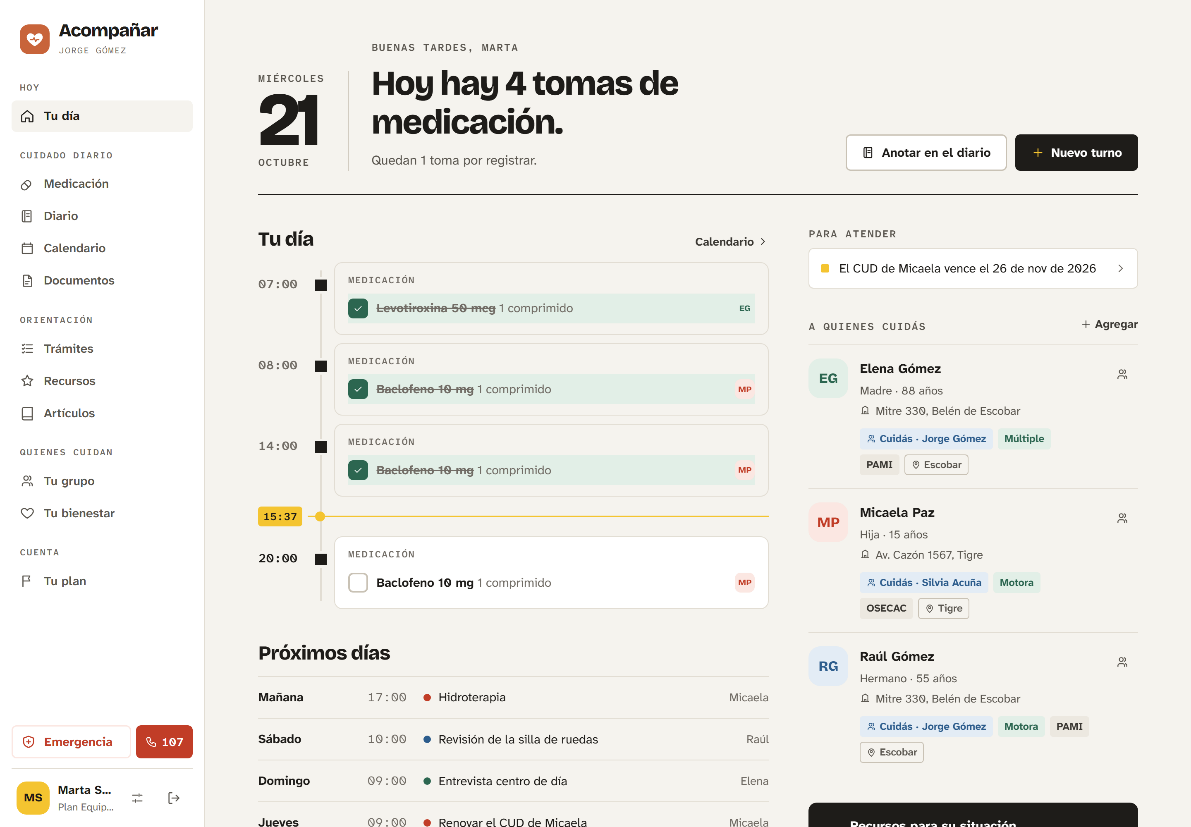
\includegraphics[width=\textwidth]{figuras/fig-4-1}
\caption{Tu día de una cuidadora contratada que atiende a personas de dos familias}\label{fig:fig-4-1}
\end{figure}

\begin{figure}[H]
\centering
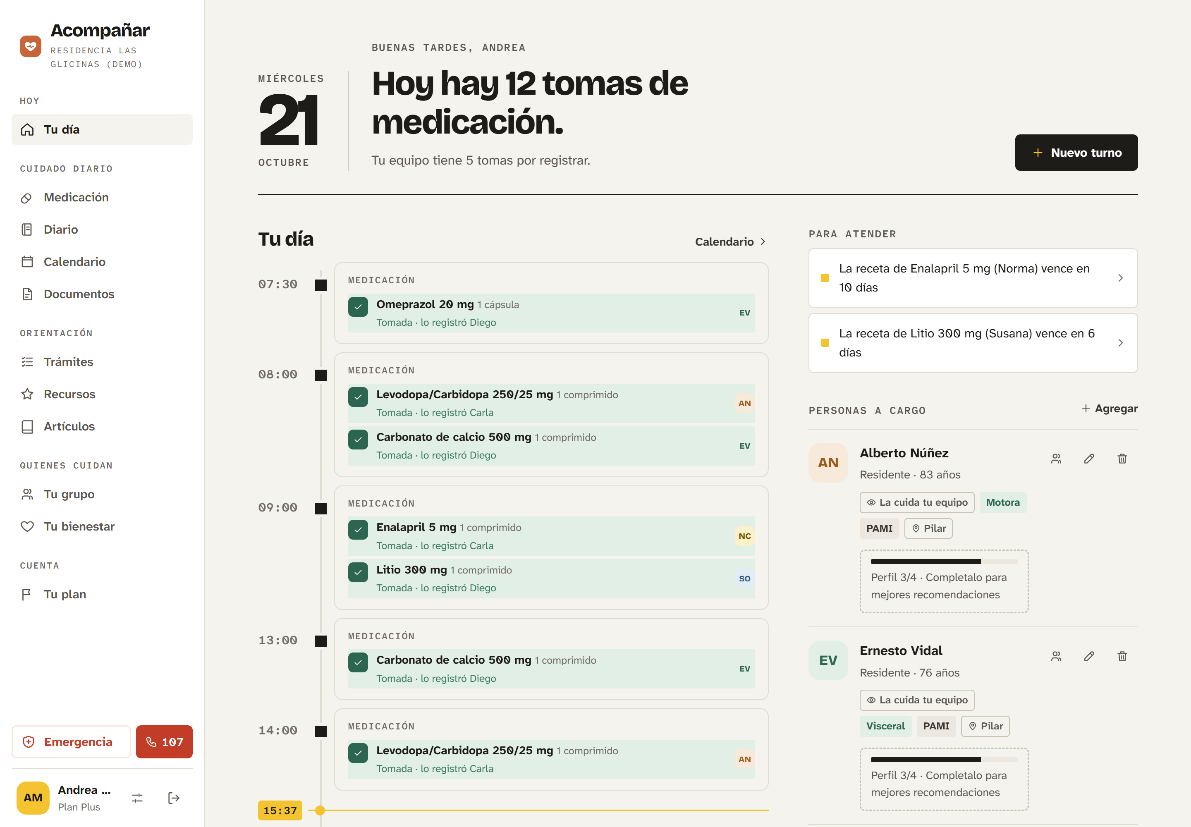
\includegraphics[width=\textwidth]{figuras/fig-4-2}
\caption{Tu día de la dueña de una residencia: el estado de cada toma y quién la registró}\label{fig:fig-4-2}
\end{figure}

\begin{figure}[H]
\centering
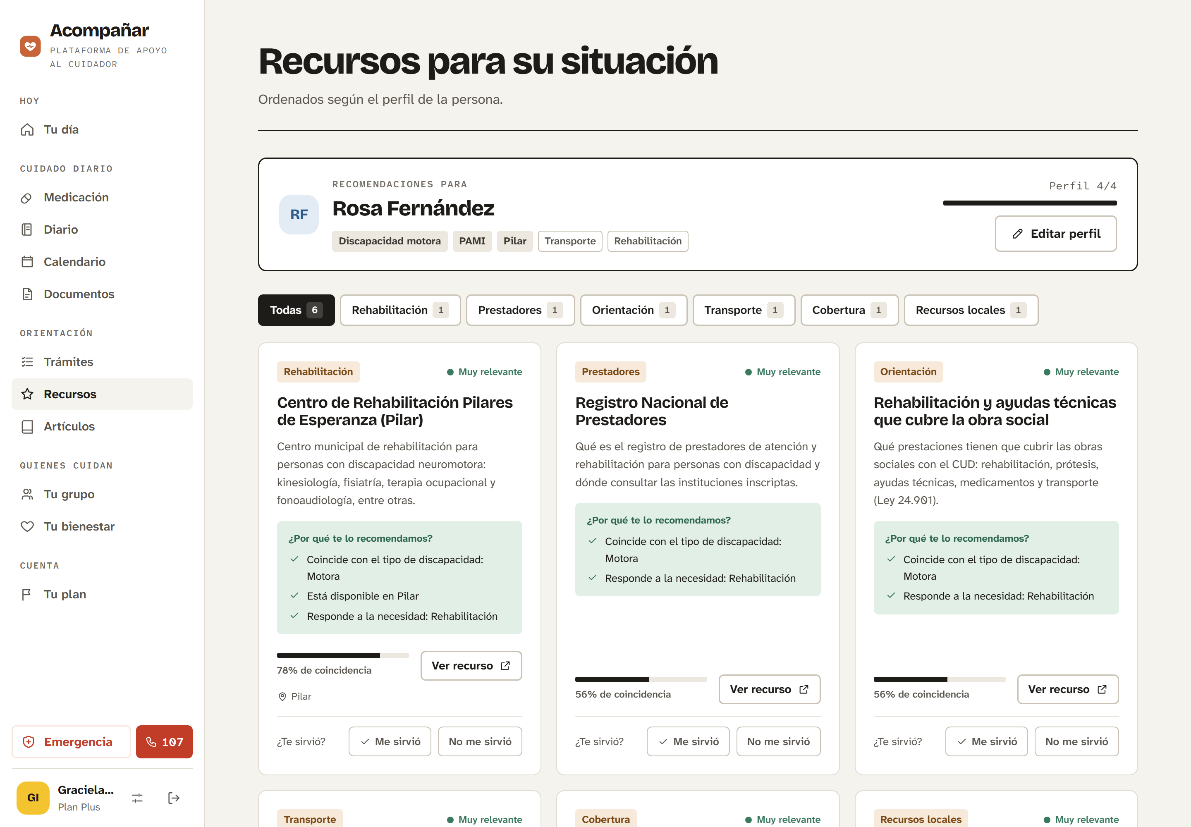
\includegraphics[width=\textwidth]{figuras/fig-4-3}
\caption{Recursos para la discapacidad de la persona, ordenados según su perfil, con su explicación y los botones de valoración}\label{fig:fig-4-3}
\end{figure}

\begin{figure}[H]
\centering
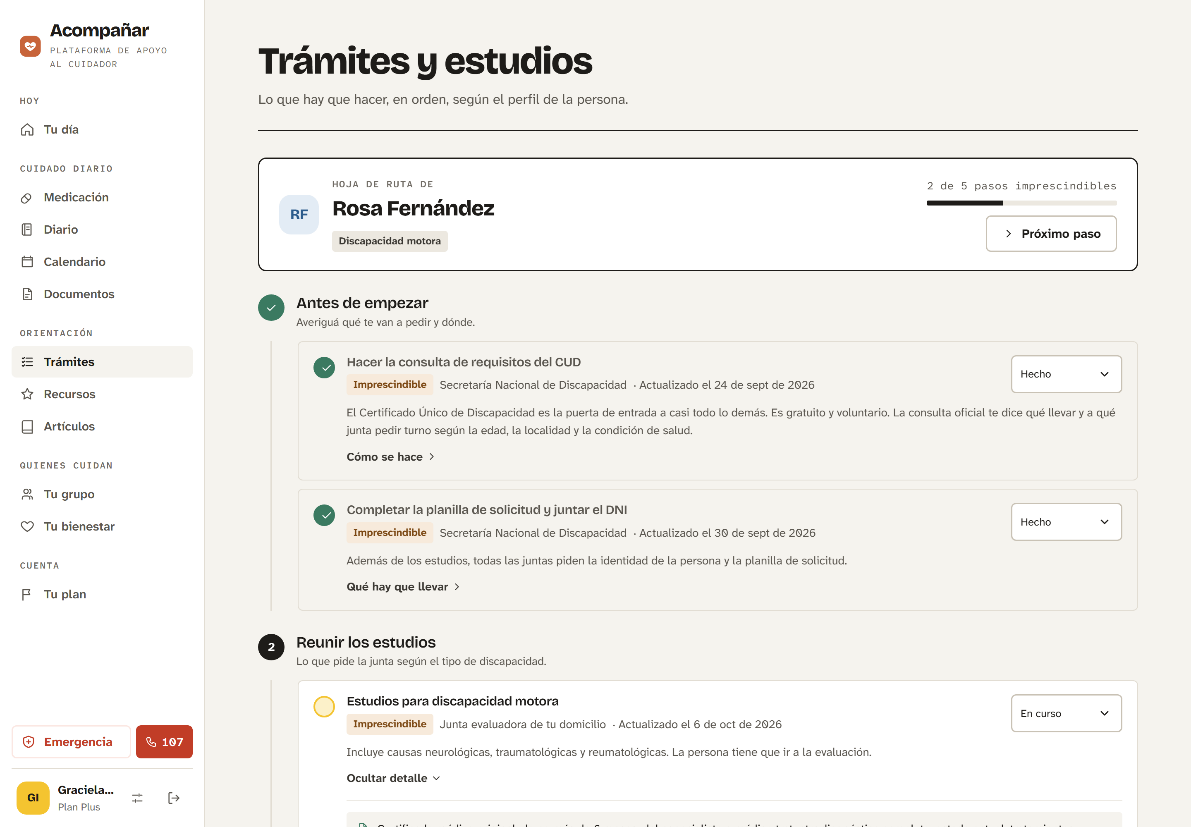
\includegraphics[width=\textwidth]{figuras/fig-4-4}
\caption{Hoja de ruta de trámites y estudios para el Certificado Único de Discapacidad}\label{fig:fig-4-4}
\end{figure}

\begin{figure}[H]
\centering
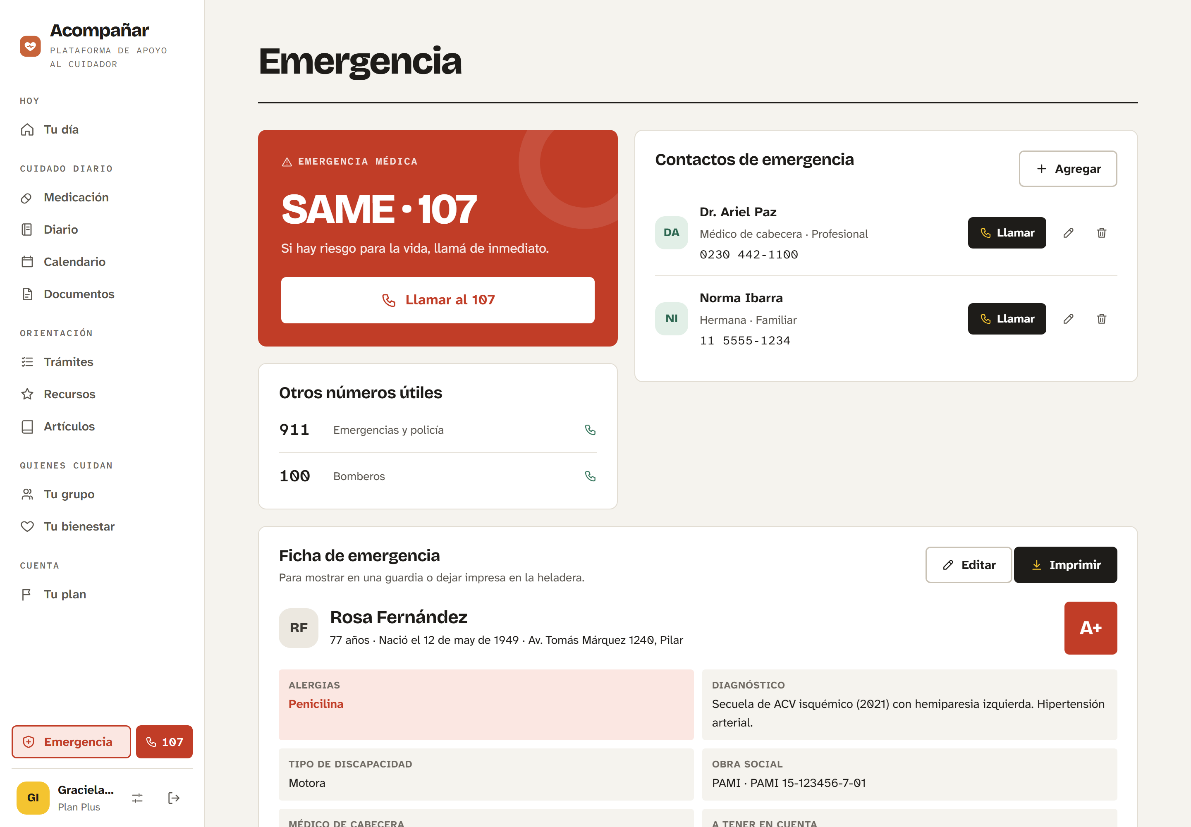
\includegraphics[width=\textwidth]{figuras/fig-4-5}
\caption{Módulo de emergencia con el acceso al 107, los contactos de la red de apoyo y la ficha}\label{fig:fig-4-5}
\end{figure}

\begin{figure}[H]
\centering
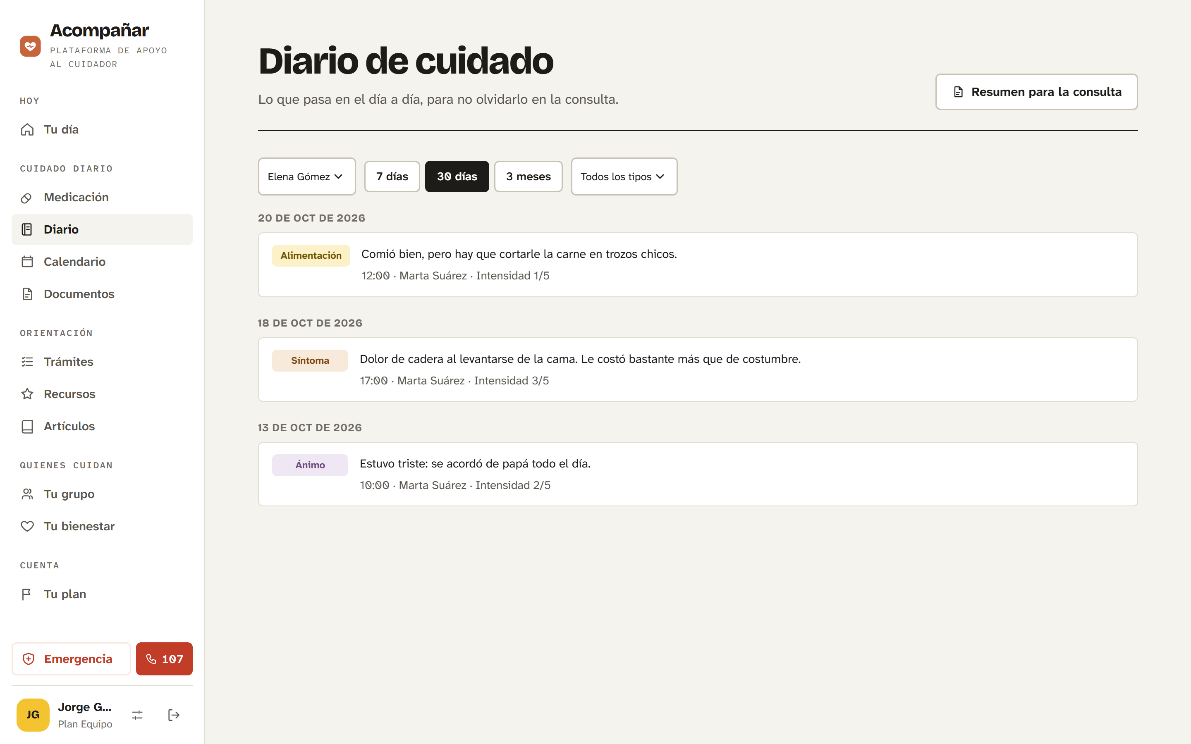
\includegraphics[width=\textwidth]{figuras/fig-4-6}
\caption{Diario visto por un familiar en modo observador. Los registros son de la cuidadora y no se pueden editar}\label{fig:fig-4-6}
\end{figure}

\begin{figure}[H]
\centering
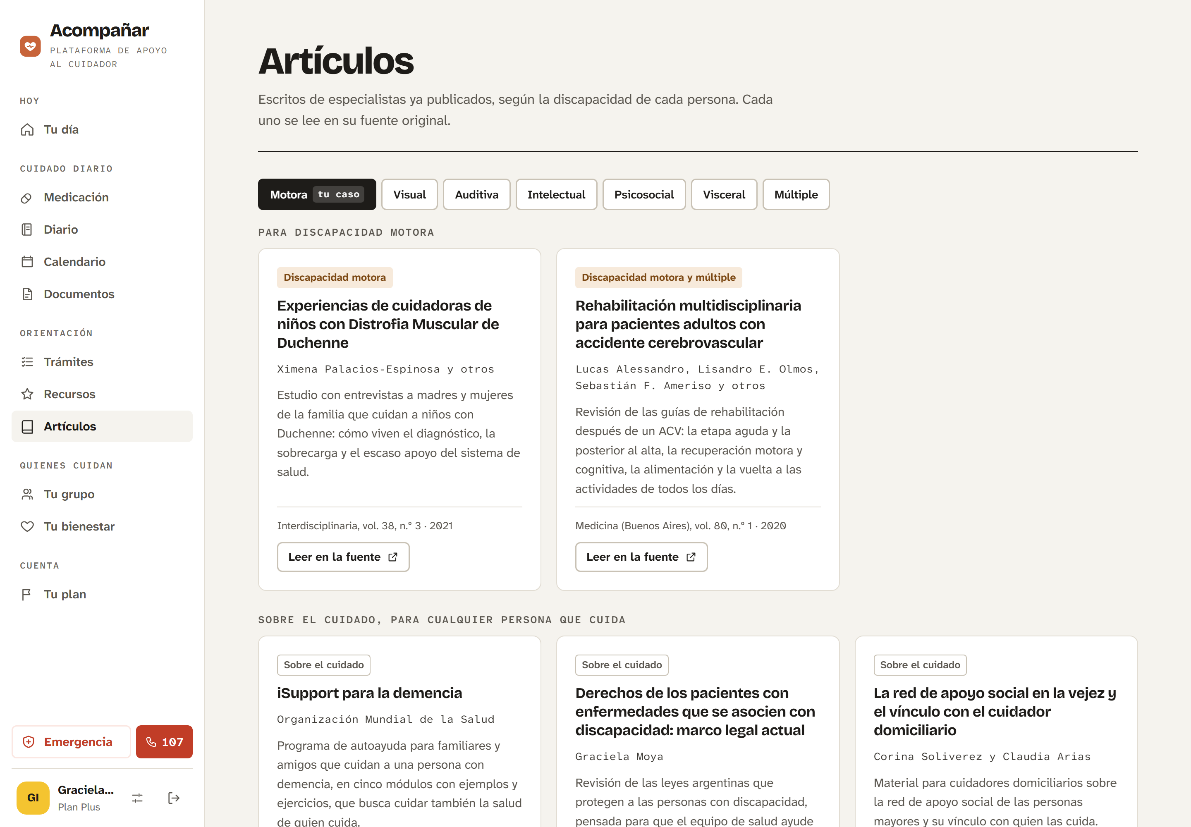
\includegraphics[width=\textwidth]{figuras/fig-4-7}
\caption{Artículos de especialistas para la discapacidad de la persona y, aparte, los generales sobre el cuidado}\label{fig:fig-4-7}
\end{figure}

\begin{figure}[H]
\centering
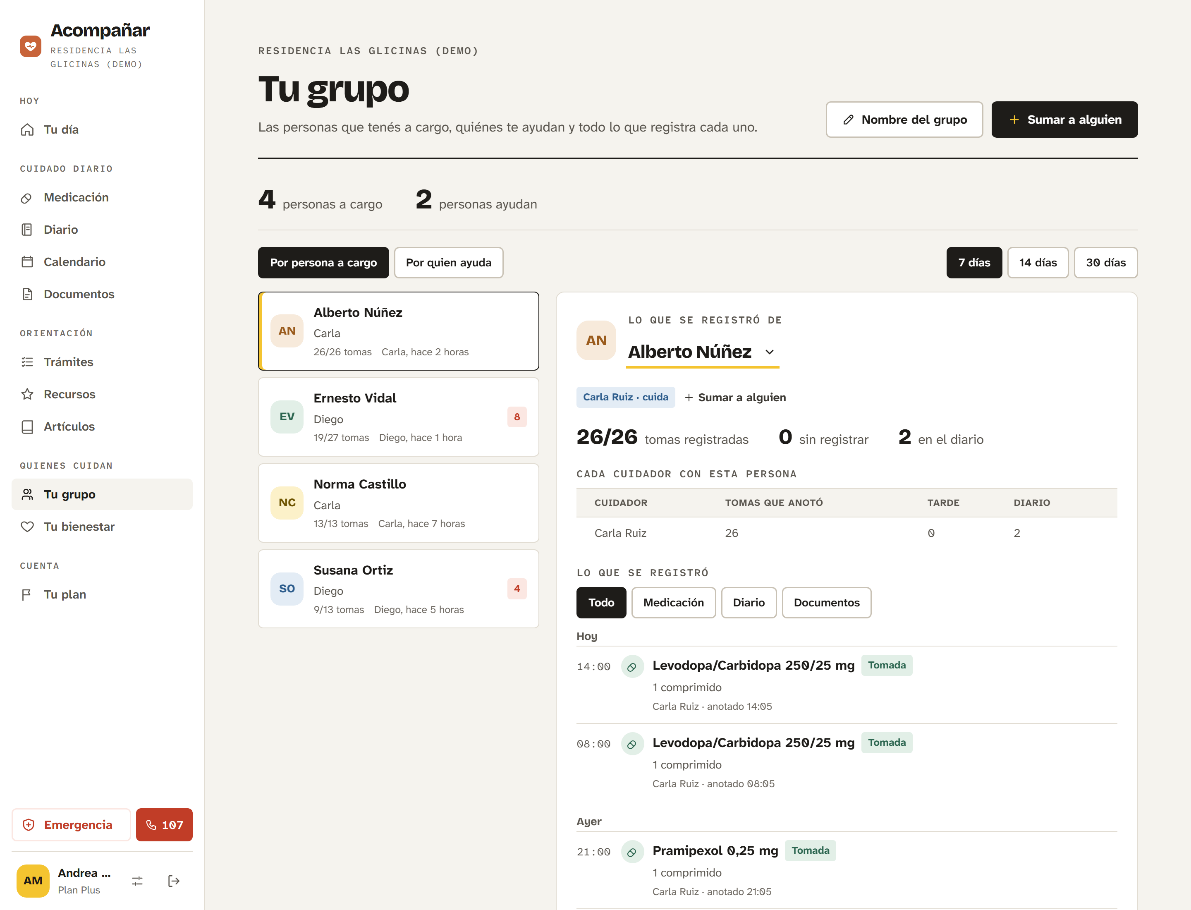
\includegraphics[width=\textwidth]{figuras/fig-4-8}
\caption{Tu grupo visto por la dueña de una residencia: cada residente, quién lo cuida y todo lo que se registró}\label{fig:fig-4-8}
\end{figure}

\begin{figure}[H]
\centering
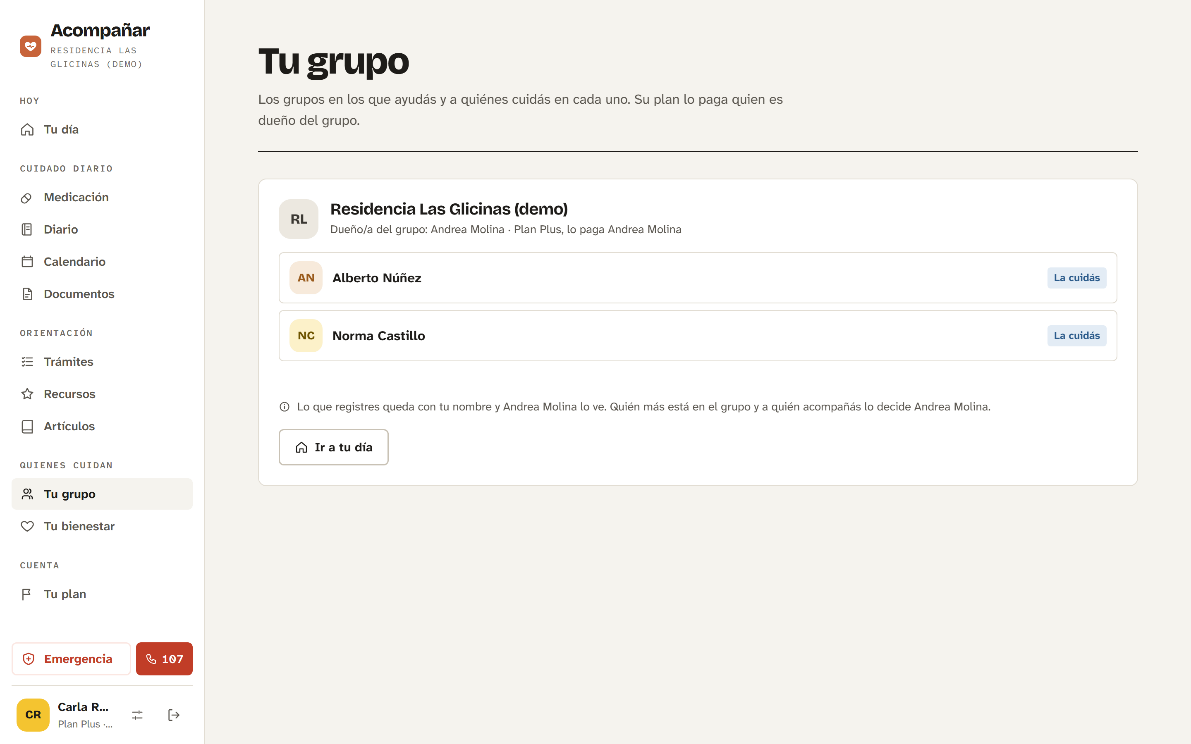
\includegraphics[width=\textwidth]{figuras/fig-4-9}
\caption{Tu grupo visto por una cuidadora: el grupo en el que ayuda, a quiénes cuida y que el plan lo paga la dueña}\label{fig:fig-4-9}
\end{figure}

\begin{figure}[H]
\centering
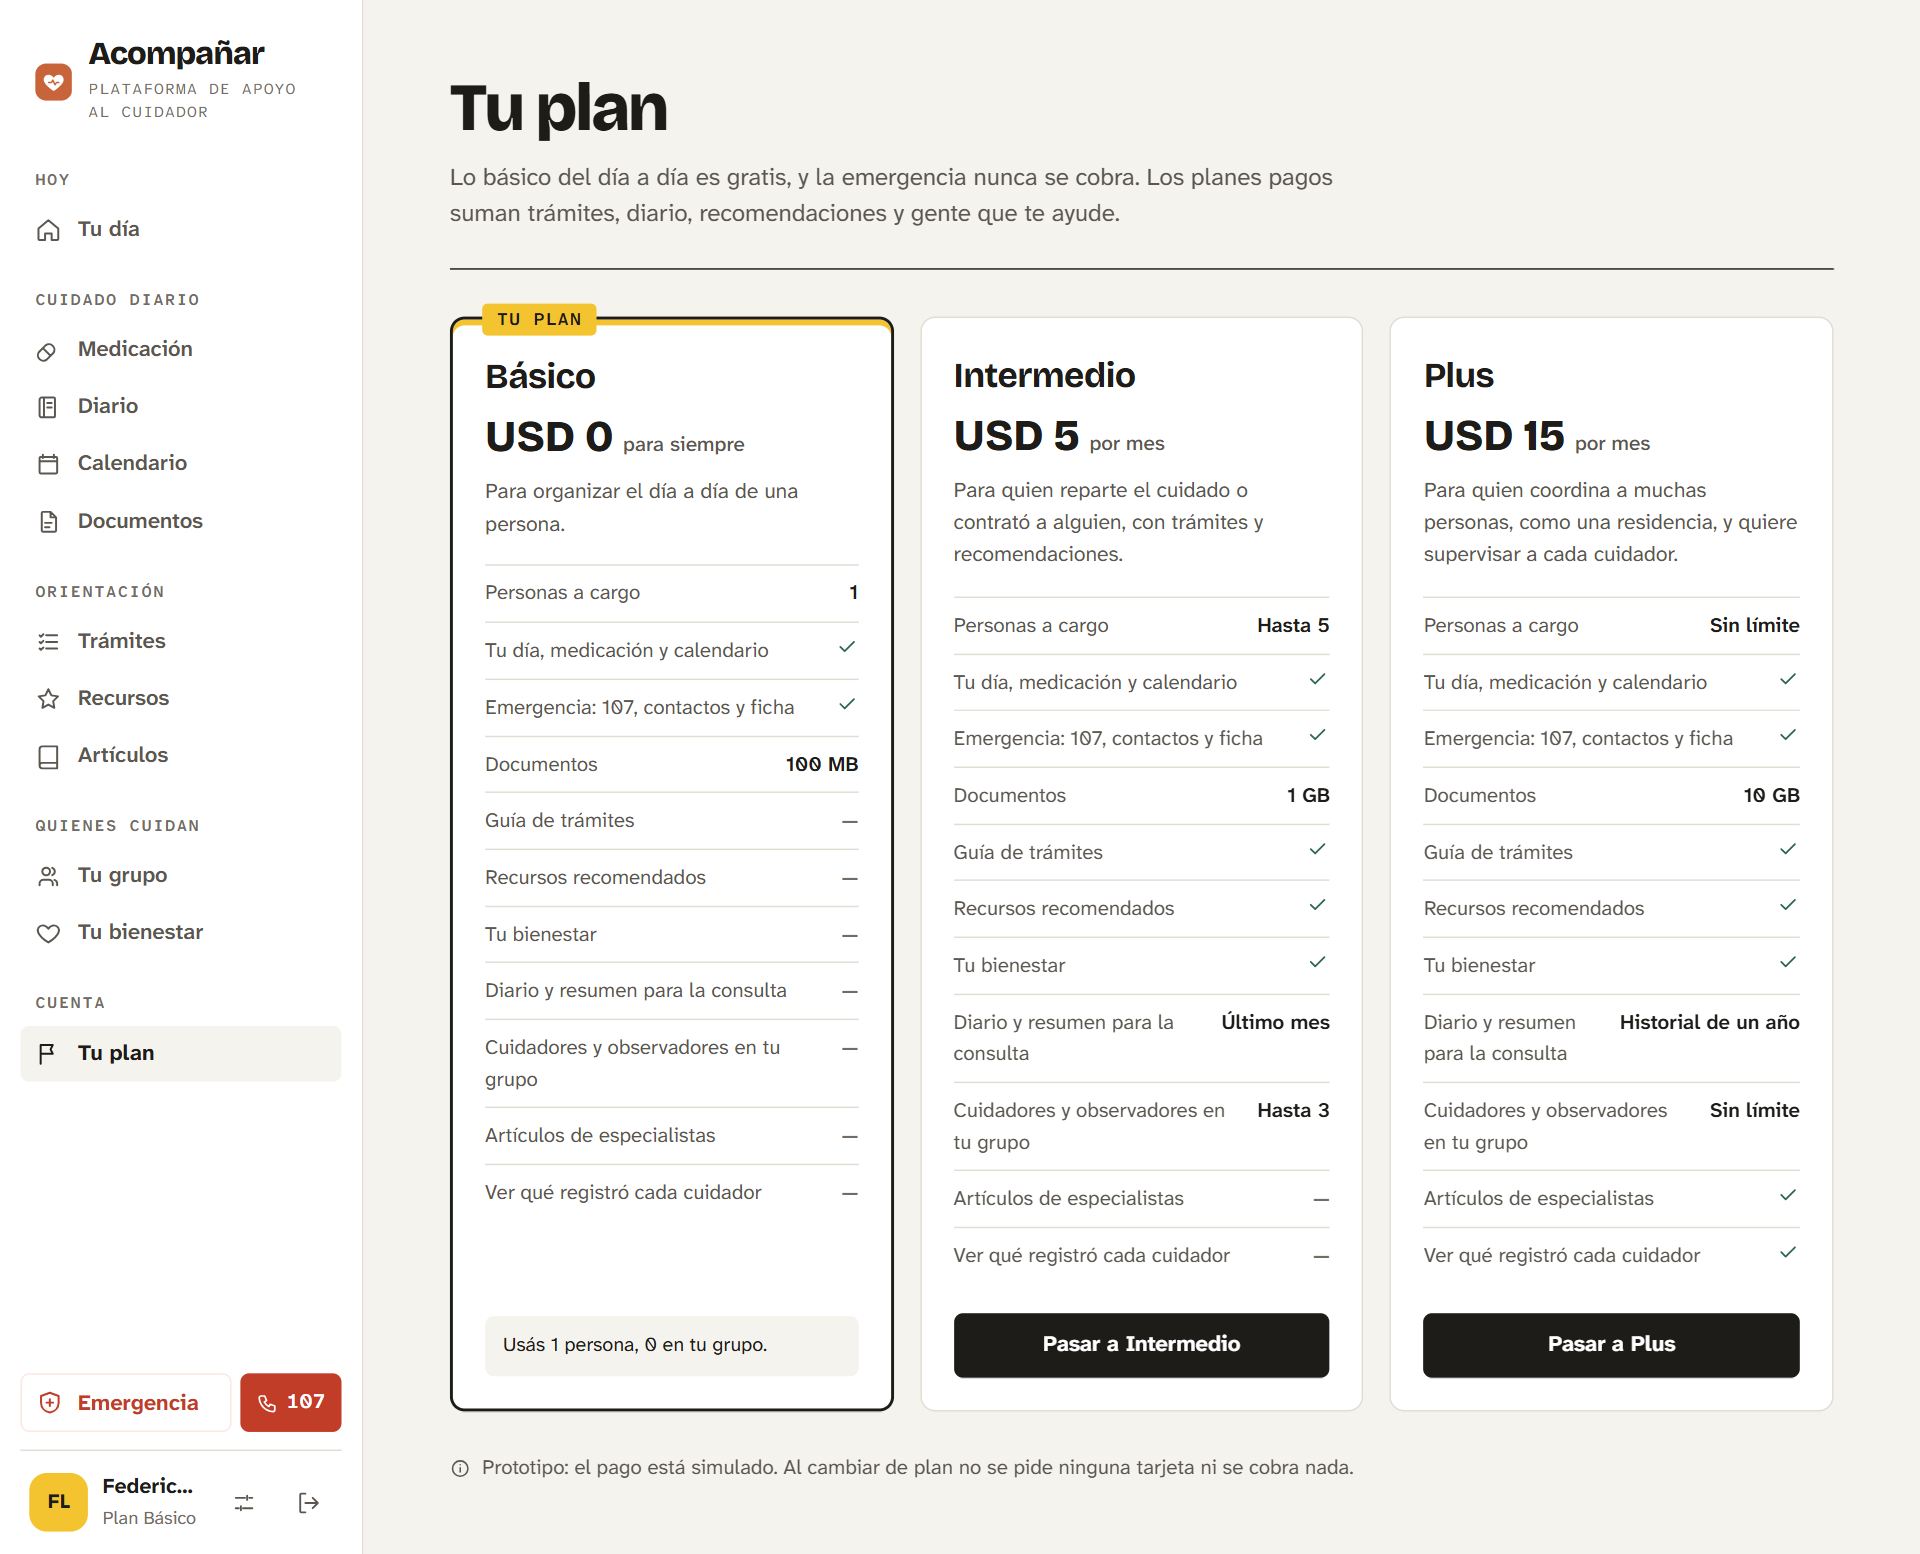
\includegraphics[width=\textwidth]{figuras/fig-4-10}
\caption{Planes Básico, Intermedio y Plus}\label{fig:fig-4-10}
\end{figure}

\begin{figure}[H]
\centering
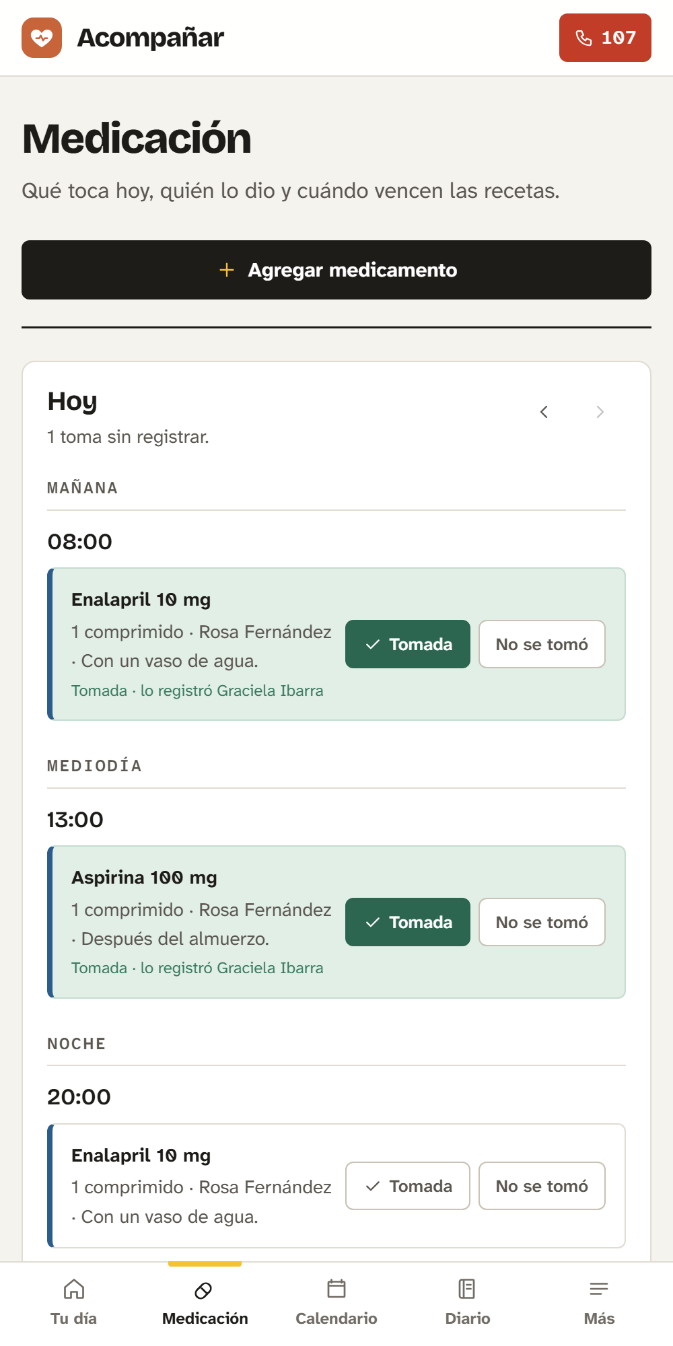
\includegraphics[width=0.35\textwidth]{figuras/fig-4-11}
\caption{Agenda de medicación en la versión para celular}\label{fig:fig-4-11}
\end{figure}

\section{Limitaciones actuales y próximos pasos}

\begin{itemize}
    \item Todavía no está publicada en la nube: Hoy la plataforma se ejecuta en un entorno local, con SQL Server Express y los datos de demostración. El próximo paso es publicarla en Azure, con la aplicación en Azure App Service y la base de datos en Azure SQL Database, para que se pueda usar desde cualquier navegador. Su comportamiento con muchos usuarios simultáneos todavía no se midió.
    \item El pago está simulado: El cambio de planes inmediato y no se cobra. Para cobrar hace falta integrar una pasarela de pagos.
    \item Faltan datos de uso reales: El componente colaborativo del recomendador está implementado, pero solo se probó con datos de demostración.
\end{itemize}

Los próximos pasos planificados son (1) validar el uso con cuidadores y con al menos una residencia, y (2) integrar una pasarela de pagos.

\section{Software}

La tabla~\ref{tab:c4-1} resume las tecnologías elegidas para la plataforma. Las versiones exactas de cada componente se detallan en el apéndice~\ref{apx:tecnicos}.

\begin{table}[H]
\centering
\caption{Tecnologías utilizadas}\label{tab:c4-1}
\small
\begin{tabularx}{\textwidth}{>{\raggedright\arraybackslash}X >{\raggedright\arraybackslash}X >{\raggedright\arraybackslash}X}
\toprule
\tb{Capa} & \tb{Tecnología elegida} & \tb{Motivo principal} \\
\midrule
Entorno de desarrollo & Visual Studio & IDE integrado con depurador y herramientas de perfilado ya conocidas. \\
Frontend web & React + Vite (JavaScript / JSX) & Interfaz reactiva y modular. Vite ofrece un entorno de desarrollo rápido sin la complejidad de un framework. \\
Backend / API & ASP.NET Core Web API (C\#, .NET 10) & Tipado fuerte, alto rendimiento y conocimiento previo, reduce errores en tiempo de compilación durante un desarrollo solitario. \\
Base de datos & SQL Server con Entity Framework Core & Motor relacional maduro y coherente con las entidades del dominio. Las migraciones versionan el esquema. \\
Documentación de API & Swagger & Documentación interactiva generada a partir del propio código de la API. \\
Autenticación & ASP.NET Core Identity y JWT & Registro, inicio de sesión, hash de contraseñas y roles integrados al framework. El token firmado identifica cada solicitud. \\
Pruebas & xUnit con SQLite en memoria & Pruebas automatizadas sobre una base relacional real que no afecta los datos del sistema. \\
Control de versiones & Git y GitHub (repositorio privado) & Historial de cambios y copia del código fuera del equipo de desarrollo. \\
\bottomrule
\end{tabularx}
\end{table}

\section{Frontend}

El frontend se construyó con React y Vite. Se eligió Vite en lugar de un framework con renderizado del lado del servidor, como Next.js, porque la plataforma no requiere ese tipo de optimización para su escala inicial, y Vite ofrece un servidor de desarrollo considerablemente más rápido con una configuración mucho más simple. La interfaz se organizó en componentes reutilizables, como las tarjetas de recomendación, la línea del día, las tarjetas de personas o los formularios.

En cuanto al acceso desde dispositivos móviles, se decidió no desarrollar una aplicación nativa separada, sino construir el frontend web como una interfaz responsive, capaz de adaptarse tanto a computadoras como a celulares desde un mismo proyecto. Esta decisión evita duplicar el desarrollo de una interfaz equivalente en una tecnología distinta. La interfaz se adapta además a lo que puede hacer cada usuario con cada persona, de modo que quien está en modo observador no ve los botones para registrar o editar.

\section{Backend y lógica de negocio}

Para la construcción de la API REST y el motor de recomendación se seleccionó ASP.NET Core Web API con C\#. La razón principal detrás de esta decisión fue el dominio previo que ya se tenía sobre estas tecnologías, lo que redujo significativamente la curva de aprendizaje y aceleró la puesta en marcha.

Trabajar con C\# ofrece una ventaja fundamental, su sistema de tipado fuerte. Esto significa que gran parte de los errores de código se detectan al momento de compilar y no cuando la aplicación ya se está ejecutando. En un escenario donde una sola persona asume todo el rol de desarrollo, pruebas y corrección de fallos, esta característica ayuda a mantener la estabilidad del sistema.

El control de acceso se concentró en un único servicio, que define qué puede hacer cada usuario con cada persona y que usan todos los controladores. Hay cuatro niveles. Ver, que tienen todos los integrantes del grupo, gestionar turnos, medicación, documentos, contactos y trámites, que tienen el dueño y los cuidadores, registrar tomas y diario, que tienen los cuidadores y el dueño solo si también cuida y administrar el perfil, la ficha y el grupo, que corresponde al dueño. Los límites de cada plan se controlan también en la API, tomando el plan del dueño de cada persona.

El motor de recomendación se mantuvo simple para no sobrecargar la arquitectura. No hizo falta incorporar librerías externas de inteligencia artificial o aprendizaje automático. Se programó como un servicio interno de la API, que solo considera los recursos del tipo de discapacidad de la persona, descarta los que piden otra obra social o localidad, aplica una función de puntaje ponderado y ajusta el orden según las valoraciones.

\section{Base de datos}

Se eligió SQL Server como motor de base de datos, en conjunto con Entity Framework Core como capa de acceso a datos. El dominio del problema es naturalmente relacional, por lo que un motor SQL resulta más adecuado que una base no relacional. Entity Framework Core, al trabajar con un enfoque code-first, permite definir el modelo de datos directamente en clases de C\# y generar el esquema de base de datos junto con sus migraciones de forma versionada.

El modelo de datos organiza la información a través de entidades como Usuario (con su plan y el nombre de su grupo), Persona asistida, Integrante del grupo, Turno, Medicamento, Toma, Entrada del diario, Documento, Contacto de emergencia, Avance de trámite, Recurso, Valoración de recurso, Artículo y Evaluación de esfuerzo.

Para asegurar que los datos se mantengan consistentes y bien relacionados, se aplican claves foráneas, borrado en cascada donde corresponde e índices únicos que evitan duplicados. La evolución del esquema se gestiona mediante las migraciones de Entity Framework Core, que al guardarse junto con el código permiten volver a una versión anterior ante cualquier eventualidad. Cuando el sistema se publique en Azure, las copias de seguridad quedarán a cargo de Azure SQL Database.

\section{Infraestructura y despliegue}

Por ahora el sistema se ejecuta en un entorno local, con SQL Server Express y los datos de demostración, y su publicación queda como próximo paso. Para esa etapa se eligió Microsoft Azure: la aplicación se publicará en Azure App Service y la base de datos en Azure SQL Database. Se eligió Azure por su integración directa con .NET y SQL Server, lo que permite desplegar sin cambiar el motor de base de datos ni el código de acceso a datos, y porque ofrece planes de bajo costo para una escala inicial. Las alternativas evaluadas fueron alojar la API en un servidor virtual propio, que exigía administrar el sistema operativo y las copias de seguridad, o pasar a una base de datos distinta de SQL Server, lo que obligaba a migrar el esquema.

Una vez publicado, la escalabilidad se resolverá con las opciones del proveedor. El plan de App Service puede aumentar su capacidad o la cantidad de instancias, y la base de datos puede pasar a un nivel de servicio superior sin cambiar la aplicación. Los costos de infraestructura previstos se presentan en el capítulo~\ref{cap:economica}.

El código se versiona en GitHub, y las migraciones de Entity Framework Core permiten reproducir el esquema de la base en cualquier entorno. El repositorio no incluye todavía un proceso automatizado de integración y despliegue continuos, por lo que las pruebas automatizadas deben ejecutarse de forma manual antes de publicar cada versión. La publicación en Azure, la automatización de ese proceso y la configuración de alertas de monitoreo sobre los registros y las métricas que ofrece Azure quedan como próximos pasos. El entorno local de desarrollo, con SQL Server Express y los datos de demostración, es el que se usa hoy para las pruebas y la demostración.

\section{Diseño y experiencia de usuario (UX/UI)}

Las decisiones de diseño aplican directamente los principios de diseño centrado en el usuario descriptos en el Capítulo 3, en particular la norma ISO 9241-210. Dado que la plataforma está pensada para cuidadores con niveles de familiaridad tecnológica muy dispares, se priorizó un lenguaje claro y directo, una navegación persistente (barra lateral en la versión de escritorio, barra inferior en la versión móvil) y la reducción del número de pasos necesarios para completar cualquier acción.

La identidad visual combina un fondo cálido, tipografía oscura y un solo color de acento, amarillo, que marca lo que requiere atención, como la hora actual o la sección activa. El rojo se reserva para la emergencia y cada persona asistida tiene un color propio, para reconocer a quién corresponde cada turno o toma. Se adoptó la tipografía Atkinson Hyperlegible, desarrollada por el Braille Institute \citep{braille2019} para personas con baja visión, y la plataforma permite agrandar el texto y activar un modo de alto contraste. El elemento de diseño más relevante sigue siendo la explicación ``¿Por qué te lo recomendamos?'' en cada recomendación, que responde a la necesidad de explicabilidad.

\section{Seguridad}

La autenticación de usuarios se implementó con ASP.NET Core Identity, el sistema de identidad integrado al propio framework, que gestiona el registro, el inicio de sesión, la recuperación de la contraseña y el hash seguro de contraseñas. Cada sesión se identifica mediante un token JWT firmado, emitido por la API tras un inicio de sesión exitoso y validado en cada solicitud posterior. Después de cinco intentos fallidos la cuenta se bloquea durante cinco minutos.

El control de accesos combina los roles de la cuenta (cuidador y administración) con el nivel de acceso de cada usuario sobre cada persona asistida, descripto en la sección de backend. Así, un cuidador contratado solo ve a las personas que tiene asignadas, un observador no puede modificar nada y nadie ve las personas del grupo de otro dueño. Los archivos que se suben se validan por su contenido real y no solo por su extensión.

El cifrado queda previsto para la publicación en Azure: allí los datos se guardarán cifrados en reposo mediante Transparent Data Encryption, que Azure SQL Database aplica de forma nativa, y viajarán cifrados con HTTPS/TLS. En el entorno local actual, que solo usa datos de demostración, no se aplica cifrado en reposo. Queda previsto reforzar la protección a nivel de base de datos mediante Row-Level Security de SQL Server. Dado que la plataforma maneja información sensible sobre la salud de terceros, el tratamiento de los datos se ajustará a lo previsto por la Ley 25.326 de Protección de Datos Personales.


    %!TEX root = ../main.tex

\chapter{Justificación económica}\label{cap:economica}

\section{Introducción}

En este capítulo se aborda el análisis económico y financiero del ``Sistema inteligente de recomendación para la gestión del cuidado de personas con discapacidad en Argentina''. El propósito central es detallar los recursos monetarios que exige la propuesta, definir las estrategias necesarias para garantizar su sostenibilidad una vez concluida la fase universitaria y determinar las condiciones bajo las cuales el proyecto resulta económicamente viable.

Para lograr una estimación certera, la evaluación distingue claramente entre el desarrollo del prototipo académico y su eventual implementación en un entorno de producción real. Durante la etapa del prototipo, no se asigna un valor monetario a las horas de trabajo dedicadas a la investigación, el diseño de software, la programación ni al trabajo de campo. Al tratarse de actividades enmarcadas en el ámbito académico, representan un esfuerzo técnico e intelectual que no implica un desembolso directo para el proyecto. En consecuencia, la inversión considerada en esta fase inicial se limita exclusivamente a los gastos monetarios imprescindibles para contratar los servicios digitales y la infraestructura tecnológica que hacen posible el funcionamiento del sistema.

\section{Metodología y alcance}

La factibilidad del proyecto se analiza mediante un flujo de fondos proyectado a cinco años y expresado en dólares estadounidenses. Para evaluar la rentabilidad financiera de la propuesta, se utilizan como indicadores clave el flujo de fondos, el período de repago, el período de repago descontado, el Valor Actual Neto (VAN) y la Tasa Interna de Retorno (TIR). Adicionalmente, se incorpora el cálculo del punto de equilibrio, el cual funciona como una referencia para identificar el nivel mínimo de ingresos que el sistema debe generar para cubrir sus costos operativos.

La decisión de estructurar la evaluación en dólares responde a que los principales servicios tecnológicos e infraestructura en la nube cotizan habitualmente en esta moneda.

\section{Análisis de mercado y competidores}

\subsection{Tamaño del mercado}

Según el INDEC, el 10,2~\% de la población de 6 años y más que vive en localidades urbanas tiene alguna discapacidad \citep{indec2018}. El Registro Nacional de Personas con Discapacidad contabilizaba, a noviembre de 2023, 1.680.723 personas con el Certificado Único de Discapacidad vigente \citep{andis2023}. Esta cifra se toma como una cota inferior del mercado potencial, porque cada persona certificada suele tener al menos una persona que la cuida, y porque no incluye a quienes no tramitaron el certificado.

El mercado se divide en tres segmentos. El primero son las personas que cuidan solas a un familiar, que usan el plan gratuito. El segundo son las familias que reparten el cuidado entre varias personas o contrataron a un cuidador, a las que se dirige el plan Intermedio. El tercero son las clínicas, residencias y centros de día, que necesitan supervisar el trabajo de varios empleados y contratan el plan Plus. El modelo de negocio es, por lo tanto, B2C para las familias y B2B para las instituciones, con una base gratuita.

La meta del escenario base es conservadora. Al quinto año proyecta 205 suscripciones pagas, lo que equivale a alrededor del 0,012~\% de las personas con certificado vigente.

\subsection{Competidores y precios de referencia}

\begin{table}[H]
\centering
\caption{Competidores y precios de referencia}\label{tab:c5-competidores}
\small
\begin{tabularx}{\textwidth}{l >{\raggedright\arraybackslash}X >{\raggedright\arraybackslash}X}
\toprule
\tb{Producto} & \tb{Modelo y precio} & \tb{Diferencia con la propuesta} \\
\midrule
CaringBridge & Gratuito, sostenido por donaciones \citep{caringbridge} & Comunicación con la red de apoyo, sin gestión del cuidado ni orientación \\
Lotsa Helping Hands & Gratuito \citep{lotsa} & Coordinación de tareas, sin registro por persona ni orientación \\
Medisafe & Suscripción de USD 4,99 por mes o USD 39,99 por año fuera de Estados Unidos desde 2026 \citep{medisafe2026} & Solo adherencia a la medicación \\
Acompañar & Plan Básico gratis con lo esencial, Intermedio USD 5 y Plus USD 15 por mes & Integra organización, grupo, trámites del contexto argentino y recomendaciones explicadas \\
\bottomrule
\end{tabularx}
\end{table}

El precio del plan Intermedio se ubica en el mismo nivel que la suscripción de Medisafe, que resuelve solo una parte del cuidado, y los productos gratuitos no cubren la gestión ni la orientación. Esto respalda la decisión de mantener gratis lo esencial y cobrar por la coordinación del grupo y la orientación.

\section{Modelo de ingresos propuesto}

La plataforma adopta un modelo de suscripción con una base gratuita y dos planes pagos. Lo básico del día a día, la línea del día, la medicación, el calendario, los documentos y la emergencia, es gratis siempre, y la emergencia nunca se cobra. Los planes pagos suman la guía de trámites, el diario, los recursos recomendados y la posibilidad de sumar cuidadores y observadores al grupo, cada uno con su propia cuenta.

Quien paga es el dueño del grupo, ya sea una familia o una institución. Las clínicas, residencias y centros de día contratan el plan Plus, que no tiene límite de pacientes ni de empleados e incluye el panel para supervisar lo que registra cada uno. Los cuidadores que forman parte de un grupo no pagan nada, porque los cubre el plan de su dueño.

\begin{table}[H]
\centering
\caption{Planes de la plataforma}\label{tab:c5-1}
\small
\begin{tabularx}{\textwidth}{l l >{\raggedright\arraybackslash}X}
\toprule
\tb{Plan} & \tb{Precio} & \tb{Qué incluye} \\
\midrule
Básico & USD 0 (gratis) & Una persona a cargo, cuidada por quien tiene la cuenta. Tu día, medicación, calendario, documentos (100 MB) y emergencia. \\
Intermedio & USD 5 por mes & Hasta cinco personas a cargo y tres integrantes en el grupo. Suma guía de trámites, diario con resumen del último mes, recursos recomendados, tu bienestar y documentos (1 GB). \\
Plus & USD 15 por mes & Personas e integrantes sin límite, artículos de especialistas, cumplimiento de cada cuidador, historial de un año y documentos (10 GB). Es el plan de las clínicas y residencias. \\
\bottomrule
\end{tabularx}
\end{table}

Para la proyección se contempla una adopción gradual de suscripciones pagas. Las cantidades corresponden a promedios anuales y no incluyen las cuentas gratuitas, que no generan ingresos. En el plan Plus se cuentan tanto familias que coordinan a muchas personas como instituciones.

\begin{table}[H]
\centering
\caption{Proyección de suscripciones e ingresos (escenario base)}\label{tab:c5-2}
\footnotesize
\begin{tabularx}{\textwidth}{l l l l l l}
\toprule
\tb{Año} & \tb{Plan Intermedio} & \tb{Plan Plus} & \tb{Ingresos Intermedio} & \tb{Ingresos Plus} & \tb{Ingresos totales} \\
\midrule
1 & 15 & 6 & USD 900 & USD 1.080 & USD 1.980 \\
2 & 35 & 15 & USD 2.100 & USD 2.700 & USD 4.800 \\
3 & 65 & 28 & USD 3.900 & USD 5.040 & USD 8.940 \\
4 & 100 & 45 & USD 6.000 & USD 8.100 & USD 14.100 \\
5 & 140 & 65 & USD 8.400 & USD 11.700 & USD 20.100 \\
\bottomrule
\end{tabularx}
\end{table}

Quien cuida a una persona por su cuenta puede usar la plataforma sin pagar. Pagan quienes necesitan más, las familias que reparten el cuidado o contrataron a alguien y las instituciones, que obtienen un valor operativo directo al poder supervisar el cuidado que brindan sus empleados. Hacia el quinto año, el plan Plus representa el 58~\% de los ingresos.

\section{Inversión inicial}

La inversión inicial contemplada para el proyecto se enfoca de manera exclusiva en los gastos monetarios estrictamente necesarios para poner en funcionamiento la infraestructura digital que requiere el sistema. Para mantener una estimación transparente del prototipo, dentro de este cálculo no se incluyen sueldos ni el costo de oportunidad del tiempo que se dedicó al proyecto. De la misma manera, se dejan fuera la compra de equipos informáticos y todo el trabajo de campo.

El monto total de esta inversión resulta sumamente accesible debido a que el desarrollo se llevó a cabo en un marco académico, un contexto que permitió aprovechar herramientas de uso gratuito, licencias educativas y servicios tecnológicos de muy bajo costo. En caso de querer dar el salto hacia una implementación comercial, van a surgir otros gastos operativos, logísticos y de infraestructura que superan el alcance de esta primera etapa universitaria.

\begin{table}[H]
\centering
\caption{Inversión inicial}\label{tab:c5-3}
\small
\begin{tabularx}{\textwidth}{>{\raggedright\arraybackslash}X l}
\toprule
\tb{Concepto} & \tb{Importe estimado} \\
\midrule
Dominio y configuración inicial & USD 25 \\
Configuración inicial de servicios cloud & USD 50 \\
Servicios digitales complementarios & USD 25 \\
\textbf{Total inversión inicial} & \textbf{USD 100} \\
\bottomrule
\end{tabularx}
\end{table}

\section{Inversión valorizada por rol y tiempo}

Aunque las horas de trabajo no implicaron un desembolso, la cátedra pide valorizar la inversión por rol y tiempo. Para hacerlo se estimaron las horas dedicadas a cada actividad y se les asignó el rol que las realizaría en un equipo. Como todo el trabajo lo hizo una sola persona con perfil junior, se usa una tarifa única de referencia de USD 7 por hora, que corresponde a un perfil junior en modalidad remota en Argentina y es una estimación propia. Un equipo con perfiles de mayor experiencia tendría un costo más alto.

\begin{table}[H]
\centering
\caption{Inversión inicial valorizada por rol}\label{tab:c5-roles}
\small
\begin{tabularx}{\textwidth}{l >{\raggedright\arraybackslash}X r r}
\toprule
\tb{Rol} & \tb{Actividades} & \tb{Horas} & \tb{Importe} \\
\midrule
Analista e investigadora & Investigación, encuesta, marco teórico y redacción de los capítulos & 210 & USD 1.470 \\
Diseñadora UX/UI & Diseño de la interfaz y prototipo & 100 & USD 700 \\
Desarrolladora backend & API, motor de recomendación y modelo de datos & 250 & USD 1.750 \\
Desarrolladora frontend & Interfaz en React & 150 & USD 1.050 \\
QA y despliegue & Pruebas, despliegue y documentación & 80 & USD 560 \\
\midrule
\textbf{Subtotal de horas} & & \textbf{790} & \textbf{USD 5.530} \\
Infraestructura inicial & Tabla~\ref{tab:c5-3} & & USD 100 \\
\textbf{Inversión total valorizada} & & & \textbf{USD 5.630} \\
\bottomrule
\end{tabularx}
\end{table}

El flujo de fondos de las secciones siguientes considera solo la inversión monetaria de USD 100, porque es el único gasto de dinero que requiere la puesta en marcha, es decir, la publicación del sistema en Azure, prevista como próximo paso. Para medir el efecto de valorizar las horas, en el análisis de escenarios se recalculan los indicadores con la inversión total de USD 5.630.

\section{Costos de operación y escalabilidad}

Una vez que el proyecto se publique y se ponga en marcha, los costos operativos se enfocan principalmente en la infraestructura en la nube, el mantenimiento del dominio junto con sus servicios auxiliares, el consumo de servicios externos y las comisiones de la pasarela de pagos. Para estas últimas se reserva un 7~\% de lo cobrado, como supuesto de trabajo.

Las cifras consideradas son reservas presupuestarias pensadas para un escenario de pequeña escala, y de ninguna manera representan presupuestos cerrados o contratos firmados. De cara a una etapa de producción real, va a ser indispensable revisar los planes vigentes de cada proveedor, contemplando sus límites de uso, las comisiones, los impuestos aplicables y el consumo efectivo que demande la plataforma.

\begin{table}[H]
\centering
\caption{Costos de operación proyectados}\label{tab:c5-5}
\footnotesize
\begin{tabularx}{\textwidth}{>{\raggedright\arraybackslash}X l l l l l}
\toprule
\tb{Concepto} & \tb{Año 1} & \tb{Año 2} & \tb{Año 3} & \tb{Año 4} & \tb{Año 5} \\
\midrule
Infraestructura cloud & USD 180 & USD 240 & USD 360 & USD 480 & USD 720 \\
Dominio, correo y auxiliares & USD 60 & USD 60 & USD 75 & USD 90 & USD 120 \\
Servicios externos y APIs & USD 60 & USD 90 & USD 150 & USD 240 & USD 360 \\
Comisiones de cobro (7~\%) & USD 139 & USD 336 & USD 626 & USD 987 & USD 1.407 \\
\textbf{Total costos} & \textbf{USD 439} & \textbf{USD 726} & \textbf{USD 1.211} & \textbf{USD 1.797} & \textbf{USD 2.607} \\
\bottomrule
\end{tabularx}
\end{table}

\section{Beneficios esperados}

Los beneficios económicos directos del proyecto provienen de las suscripciones. A la par de estos retornos, el sistema genera importantes beneficios de carácter social y operativo, aunque estos no se monetizan en la evaluación económica dada la falta de información objetiva para asignarles un valor financiero preciso. Esta decisión de dejar fuera del VAN los beneficios intangibles responde a un criterio de prudencia metodológica.

\begin{table}[H]
\centering
\caption{Beneficios esperados}\label{tab:c5-6}
\small
\begin{tabularx}{\textwidth}{l >{\raggedright\arraybackslash}X >{\raggedright\arraybackslash}X}
\toprule
\tb{Tipo} & \tb{Beneficio} & \tb{Consideración} \\
\midrule
Tangible & Ingresos por suscripciones a los planes Intermedio y Plus & Incluido en el flujo \\
Tangible & Menor tiempo destinado a buscar información & Medible durante una prueba piloto \\
Intangible & Información organizada y centralizada & Evaluación mediante percepción de utilidad \\
Intangible & Recomendaciones adaptadas a cada discapacidad & Satisfacción con la relevancia y valoraciones \\
Intangible & Coordinación del grupo de cuidado y supervisión a distancia & Uso del modo observador y del panel del grupo \\
Intangible & Mayor acceso a recursos y trámites & Uso de recursos recomendados y avance de trámites \\
\bottomrule
\end{tabularx}
\end{table}

\section{Flujo de fondos proyectado}

El flujo de fondos refleja las entradas y salidas de dinero que se estiman para todo el horizonte del análisis. El año cero concentra la inversión inicial imprescindible para poner en marcha la plataforma, mientras que los períodos posteriores muestran la evolución de los ingresos, los costos operativos y el flujo neto de caja al cierre de cada ejercicio.

El saldo neto anual es positivo desde el primer año de funcionamiento. Esto se explica por la baja inversión inicial, por los costos operativos acotados y por el supuesto de concretar veintiuna suscripciones pagas durante los primeros doce meses.

\begin{table}[H]
\centering
\caption{Flujo de fondos proyectado (escenario base)}\label{tab:c5-7}
\footnotesize
\begin{tabularx}{\textwidth}{>{\raggedright\arraybackslash}X l l l l l l}
\toprule
\tb{Concepto} & \tb{Año 0} & \tb{Año 1} & \tb{Año 2} & \tb{Año 3} & \tb{Año 4} & \tb{Año 5} \\
\midrule
Ingresos & USD 0 & USD 1.980 & USD 4.800 & USD 8.940 & USD 14.100 & USD 20.100 \\
Costos operativos & USD 0 & USD 439 & USD 726 & USD 1.211 & USD 1.797 & USD 2.607 \\
Inversión inicial & -USD 100 & USD 0 & USD 0 & USD 0 & USD 0 & USD 0 \\
Flujo neto & -USD 100 & USD 1.541 & USD 4.074 & USD 7.729 & USD 12.303 & USD 17.493 \\
\bottomrule
\end{tabularx}
\end{table}

\section{Flujo de fondos descontado}

Para calcular el Valor Actual Neto (VAN) y el período de repago descontado, cada flujo proyectado se actualiza a valor presente aplicando una tasa de descuento del 20~\% anual, mediante el factor 1/(1+0,20)\textasciicircum{}t, donde t representa el año correspondiente.

\begin{table}[H]
\centering
\caption{Flujo de fondos descontado}\label{tab:c5-8}
\small
\begin{tabularx}{\textwidth}{l l >{\raggedright\arraybackslash}X l >{\raggedright\arraybackslash}X}
\toprule
\tb{Año} & \tb{Flujo neto} & \tb{Factor de descuento} & \tb{Flujo descontado} & \tb{Acumulado descontado} \\
\midrule
0 & -100 & 1,000 & -100 & -100 \\
1 & 1.541 & 0,833 & 1.284 & 1.184 \\
2 & 4.074 & 0,694 & 2.829 & 4.013 \\
3 & 7.729 & 0,579 & 4.473 & 8.486 \\
4 & 12.303 & 0,482 & 5.933 & 14.419 \\
5 & 17.493 & 0,402 & 7.030 & 21.449 \\
\bottomrule
\end{tabularx}
\end{table}

\section{Flujo de caja acumulado y período de repago}

El flujo de caja acumulado permite identificar el momento en que se recupera la inversión inicial. Se calcula sumando los saldos netos de cada período para observar cómo se va absorbiendo la erogación inicial.

En este proyecto, la inversión se recupera durante el primer año de operación. Dado que se parte de un saldo a recuperar de USD 100 y que el flujo neto del primer año asciende a USD 1.541, la proporción necesaria para cubrir ese desembolso es de 100/1.541, es decir 0,065. Esto significa que el período de repago simple es de aproximadamente 0,07 años, menos de un mes desde la puesta en marcha de la plataforma.

\begin{table}[H]
\centering
\caption{Flujo de caja acumulado}\label{tab:c5-9}
\small
\begin{tabularx}{\textwidth}{l l l}
\toprule
\tb{Año} & \tb{Flujo neto} & \tb{Flujo acumulado} \\
\midrule
0 & -USD 100 & -USD 100 \\
1 & USD 1.541 & USD 1.441 \\
2 & USD 4.074 & USD 5.515 \\
3 & USD 7.729 & USD 13.244 \\
4 & USD 12.303 & USD 25.547 \\
5 & USD 17.493 & USD 43.040 \\
\bottomrule
\end{tabularx}
\end{table}

\begin{figure}[H]
\centering
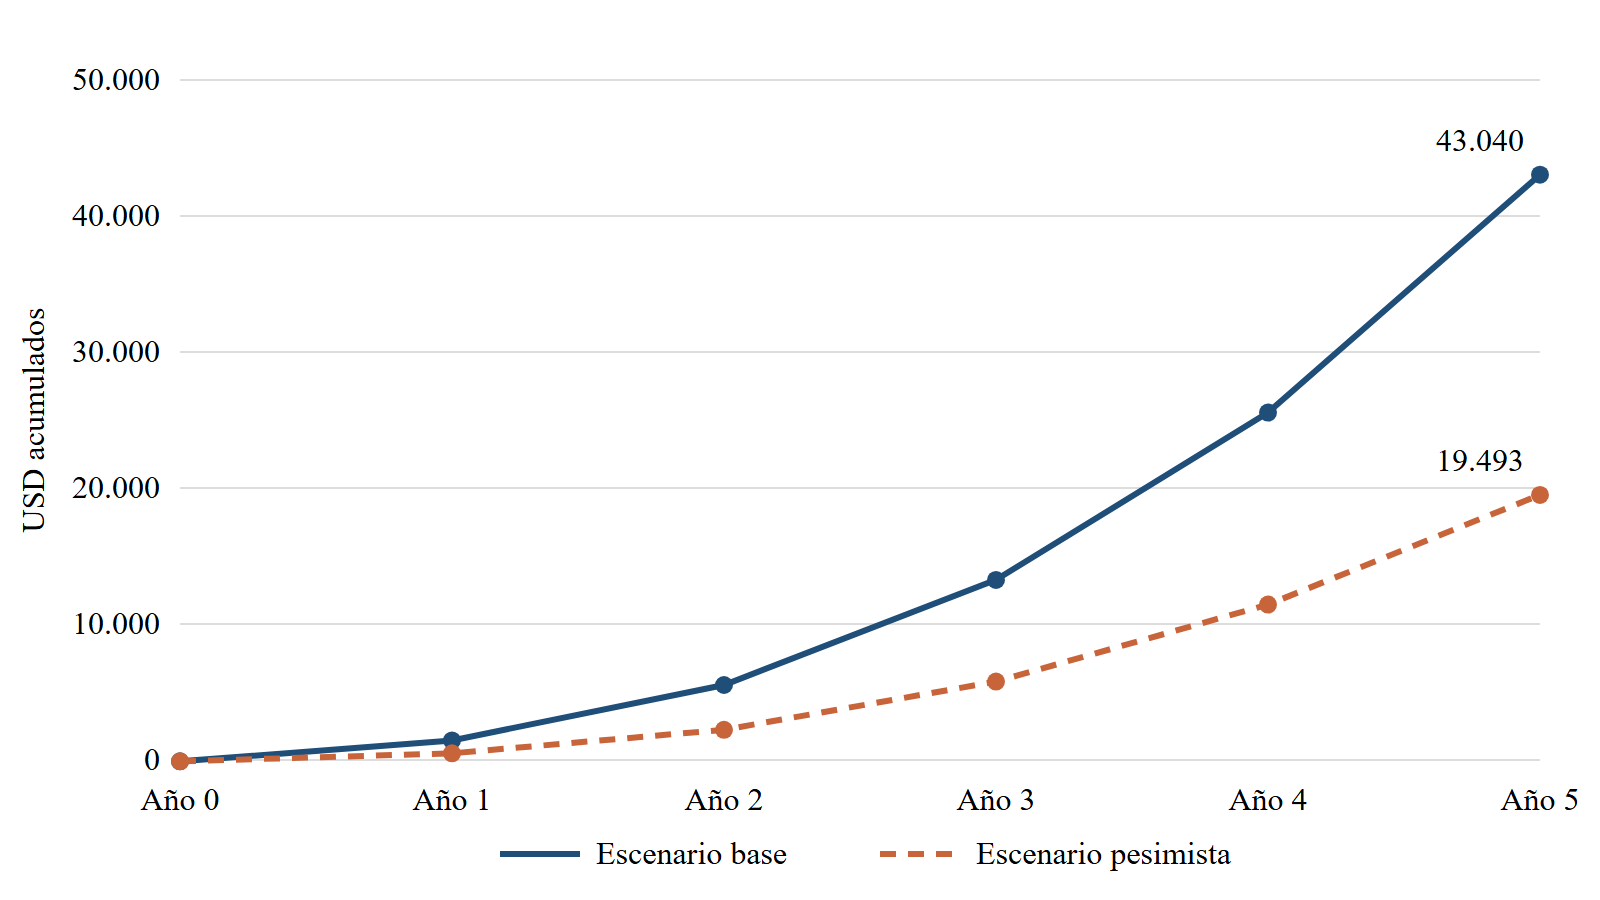
\includegraphics[width=\textwidth]{figuras/fig-5-1}
\caption{Evolución estimada del flujo de caja acumulado en el escenario base y en el pesimista}\label{fig:fig-5-1}
\end{figure}

\section{Período de repago descontado}

El período de repago descontado incorpora la tasa del 20~\% para evaluar en qué momento se recupera la inversión medida en valor presente. El flujo descontado del primer año se ubica en USD 1.284, suficiente para absorber el desembolso inicial de USD 100 dentro de esos mismos doce meses. La fracción requerida (100/1.284) es de 0,08 años, alrededor de 0,9 meses de operación.

\section{Tasa de descuento}

La tasa de descuento se construyó con el modelo de valoración de activos de capital ajustado por riesgo país, sumando una prima por la etapa temprana del proyecto:

\[
r = r_f + \beta \cdot \mathit{PRM} + \mathit{RP} + \text{prima por etapa temprana}
\]

\begin{table}[H]
\centering
\caption{Construcción de la tasa de descuento}\label{tab:c5-tasa}
\small
\begin{tabularx}{\textwidth}{>{\raggedright\arraybackslash}X r >{\raggedright\arraybackslash}X}
\toprule
\tb{Componente} & \tb{Valor} & \tb{Fuente} \\
\midrule
Tasa libre de riesgo $r_f$ (bono del Tesoro de Estados Unidos a 10 años, 15/10/2026) & 5,10~\% & \citet{fred2026} \\
Beta desapalancada del sector software, sistemas y aplicaciones, corregida por caja ($\beta$) & 1,25 & \citet{damodaran2026betas} \\
Prima de riesgo de mercado implícita, enero de 2026 ($\mathit{PRM}$) & 4,23~\% & \citet{bvr2026erp} \\
Riesgo país de Argentina, 23/10/2026 ($\mathit{RP}$) & 7,07~\% & \citet{rava2026} \\
\midrule
Costo del capital propio ($5{,}10 + 1{,}25 \times 4{,}23 + 7{,}07$) & 17,46~\% & Cálculo propio \\
Prima por etapa temprana e iliquidez & 2,54~\% & Estimación propia \\
\textbf{Tasa de descuento adoptada} & \textbf{20,00~\%} & \\
\bottomrule
\end{tabularx}
\end{table}

El proyecto no tiene deuda, por lo que la tasa coincide con el costo del capital propio. La prima por etapa temprana refleja que se trata de un proyecto sin historia de ingresos y sin un mercado secundario para su participación. Es una estimación propia y se fijó para que la tasa total quede en un valor redondo del 20~\%. El riesgo país se tomó en un momento de suba durante octubre de 2026, por lo que la tasa resulta prudente. Si el proyecto avanza hacia una etapa comercial, la tasa deberá recalcularse con los valores vigentes.

\section{Valor Actual Neto (VAN)}

Al descontar los flujos futuros con la tasa de corte del 20~\% anual y restar la inversión inicial, el VAN alcanza un resultado aproximado de USD 21.449. Al arrojar un indicador claramente superior a cero, la propuesta resulta económicamente aceptable bajo los supuestos del escenario base.

\section{Tasa Interna de Retorno (TIR)}

La Tasa Interna de Retorno (TIR) es el porcentaje de descuento que iguala el VAN a cero. Sobre el flujo proyectado, el cálculo arroja una TIR cercana al 1.694~\% anual. Este valor tan elevado no responde a un margen de ganancias desmedido, sino a que la inversión inicial considerada es muy baja en comparación con los flujos netos que se generan desde el primer año.

Por esta razón, la TIR debe interpretarse con cautela y no tomarse de forma aislada. Si bien supera ampliamente la tasa de corte del 20~\%, depende de forma directa de que se cumplan las hipótesis de adopción de los planes pagos.

\section{Punto de equilibrio}

Durante el primer año, los costos operativos fijos (sin contar las comisiones) alcanzan USD 300. Cada suscripción al plan Intermedio aporta, descontada la comisión, unos USD 55,80 al año, y cada suscripción Plus unos USD 167,40. Por lo tanto, el punto de equilibrio operativo se alcanza con seis suscripciones Intermedio, con dos suscripciones Plus o con una combinación de ambas, por ejemplo, una institución y tres familias.

Este cálculo se enfoca en la sostenibilidad operativa y no incluye la amortización del desembolso inicial, que se evalúa con los indicadores de período de repago.

\section{Análisis de escenarios}

El escenario base asume una cantidad creciente de suscripciones a los planes Intermedio y Plus en los años 1 a 5. Para evaluar si el proyecto conserva su viabilidad con una adopción mucho más lenta, se construye un escenario pesimista que reduce aproximadamente a la mitad las suscripciones pagas, manteniendo los precios y los costos fijos.

\begin{table}[H]
\centering
\caption{Escenario pesimista}\label{tab:c5-10}
\footnotesize
\begin{tabularx}{\textwidth}{>{\raggedright\arraybackslash}X l l l l l l}
\toprule
\tb{Concepto} & \tb{Año 0} & \tb{Año 1} & \tb{Año 2} & \tb{Año 3} & \tb{Año 4} & \tb{Año 5} \\
\midrule
Suscripciones (Intermedio / Plus) & 0 & 7 / 3 & 17 / 7 & 32 / 14 & 50 / 22 & 70 / 32 \\
Ingresos & USD 0 & USD 960 & USD 2.280 & USD 4.440 & USD 6.960 & USD 9.960 \\
Costos operativos & USD 0 & USD 367 & USD 550 & USD 896 & USD 1.297 & USD 1.897 \\
Flujo neto & -USD 100 & USD 593 & USD 1.730 & USD 3.544 & USD 5.663 & USD 8.063 \\
Flujo acumulado & -USD 100 & USD 493 & USD 2.223 & USD 5.767 & USD 11.430 & USD 19.493 \\
\bottomrule
\end{tabularx}
\end{table}

En el escenario pesimista, el VAN arroja un valor aproximado de USD 9.618, alrededor de un 55~\% menor que el del escenario base, pero igualmente positivo. La TIR resultante es de aproximadamente 755~\%, y el período de repago se extiende a 0,17 años (2,0 meses) en términos simples y a 0,20 años (2,4 meses) en términos descontados.

Este resultado indica que el proyecto mantiene su viabilidad económica incluso si la adopción resulta la mitad de lo proyectado. El indicador más sensible es el VAN, aunque en ambos escenarios la inversión inicial se recupera dentro del primer año.

El escenario optimista supone un 50~\% más de suscripciones que el escenario base en cada año, con los mismos precios y costos fijos. Mantener los costos fijos es un supuesto favorable, porque una mayor cantidad de usuarios podría requerir más infraestructura.

\begin{table}[H]
\centering
\caption{Escenario optimista}\label{tab:c5-optimista}
\footnotesize
\begin{tabularx}{\textwidth}{>{\raggedright\arraybackslash}X l l l l l l}
\toprule
\tb{Concepto} & \tb{Año 0} & \tb{Año 1} & \tb{Año 2} & \tb{Año 3} & \tb{Año 4} & \tb{Año 5} \\
\midrule
Suscripciones (Intermedio / Plus) & 0 & 23 / 9 & 53 / 23 & 98 / 42 & 150 / 68 & 210 / 98 \\
Ingresos & USD 0 & USD 3.000 & USD 7.320 & USD 13.440 & USD 21.240 & USD 30.240 \\
Costos operativos & USD 0 & USD 510 & USD 902 & USD 1.526 & USD 2.297 & USD 3.317 \\
Flujo neto & -USD 100 & USD 2.490 & USD 6.418 & USD 11.914 & USD 18.943 & USD 26.923 \\
Flujo acumulado & -USD 100 & USD 2.390 & USD 8.808 & USD 20.722 & USD 39.665 & USD 66.588 \\
\bottomrule
\end{tabularx}
\end{table}

La tabla~\ref{tab:c5-escenarios} resume los indicadores de los tres escenarios, primero con la inversión monetaria de USD 100 y después con la inversión valorizada de USD 5.630.

\begin{table}[H]
\centering
\caption{Indicadores de los tres escenarios}\label{tab:c5-escenarios}
\small
\begin{tabularx}{\textwidth}{l R R R R}
\toprule
 & \multicolumn{1}{r}{\tb{Inversión USD 100}} & \multicolumn{3}{c}{\tb{Inversión valorizada USD 5.630}} \\
\cmidrule(lr){2-2}\cmidrule(lr){3-5}
\tb{Escenario} & \tb{VAN} & \tb{VAN} & \tb{TIR} & \tb{Repago descontado} \\
\midrule
Pesimista & USD 9.618 & USD 4.088 & 40~\% & 3,7 años \\
Base & USD 21.449 & USD 15.919 & 79~\% & 2,3 años \\
Optimista & USD 33.282 & USD 27.752 & 109~\% & 1,8 años \\
\bottomrule
\end{tabularx}
\end{table}

Con la inversión valorizada, el VAN sigue siendo positivo en los tres escenarios y la TIR supera la tasa de corte del 20~\% en todos los casos. En el escenario pesimista la inversión se recupera recién en el cuarto año, por lo que la viabilidad depende de que la adopción no caiga por debajo de ese nivel.

\section{Alternativas consideradas}

Se evaluaron distintas alternativas de monetización. La primera versión de este análisis se basaba solo en alianzas institucionales, lo que dejaba la sostenibilidad del proyecto atada a convencer a instituciones y no reconocía que hay familias que sí obtienen un valor concreto, como coordinar a un cuidador contratado y ver lo que registra sin estar presentes.

Una versión intermedia combinaba planes para familias con un abono aparte para instituciones. Se descartó porque obligaba a tener dos tipos de cuenta distintos, cuando una residencia funciona igual que una familia grande, un dueño con varias personas a cargo y varios cuidadores.

También se analizó un modelo basado exclusivamente en publicidad. Aunque habría permitido mantener la gratuidad, su viabilidad exigía un volumen masivo de tráfico y la inclusión de anuncios corría el riesgo de saturar la interfaz en un entorno que requiere máxima claridad.

Finalmente se optó por un modelo de suscripción en tres niveles, con un plan gratuito y dos pagos. Este esquema mantiene gratis lo esencial del día a día, incluida la emergencia, cobra a quienes necesitan coordinar a más personas y sirve igual para una familia que para una institución.

\section{Análisis de impacto}

\subsection{Impacto social}

El principal impacto que busca generar la plataforma es facilitar y centralizar el acceso a la información para quienes tienen a su cargo el cuidado de personas con discapacidad. A través de la organización de los recursos disponibles, el sistema apunta a reducir la dispersión de datos, simplificar la búsqueda de soluciones y brindar recomendaciones personalizadas según las necesidades concretas de cada perfil. Al mismo tiempo, permite que el cuidado se reparta entre varias personas sin perder información, y que las familias sepan cómo se cuida a su familiar, aunque no estén presentes.

\subsection{Impacto institucional}

Para las clínicas, residencias y centros de día, la plataforma ofrece un registro ordenado del cuidado de cada paciente y una herramienta para supervisar a su personal, por ejemplo, detectando tomas de medicación que no se registraron o que se registraron tarde. Además, les permite sumar a las familias de sus pacientes como observadoras, lo que hace más transparente y fluida la comunicación con ellas.

\subsection{Impacto legal}

De cara a una implementación real, será imprescindible considerar de manera rigurosa el marco normativo aplicable a la protección de datos personales, prestando especial atención al tratamiento de información sensible vinculada con personas con discapacidad. Esto incluye definir con claridad quién puede ver la información de cada persona, qué pasa cuando un cuidador deja de trabajar con una familia y cómo se informa el uso de los datos en las instituciones. Asimismo, la plataforma funciona estrictamente como una herramienta de orientación y organización, por lo que no reemplaza en ninguna circunstancia la atención médica ni está facultada para realizar diagnósticos ni emitir prescripciones.

\subsection{Impacto ambiental}

Al tratarse de una solución 100~\% digital, la plataforma no demanda infraestructura física dedicada ni despliegues territoriales para que los usuarios puedan utilizarla. Por este motivo, el impacto ambiental directo de la propuesta es reducido. En una implementación a mayor escala, se deberá considerar la huella de carbono derivada del consumo energético del procesamiento de datos y del alojamiento continuo en servicios cloud.

\section{Supuestos y restricciones}

\begin{itemize}
    \item Los precios de los planes se mantienen constantes en dólares durante los cinco años.
    \item Las comisiones de cobro representan el 7~\% de lo facturado, como supuesto de trabajo.
    \item Los costos de infraestructura, dominio y servicios externos son reservas presupuestarias para una escala pequeña, no cotizaciones firmes.
    \item La cantidad de suscripciones de cada escenario es una estimación propia que no fue validada con familias ni con instituciones.
    \item El valor hora usado para valorizar la inversión es una estimación propia para un perfil junior.
    \item No se consideran impuestos ni la amortización de equipos informáticos.
    \item El proyecto no toma deuda, se financia con el aporte inicial y con los ingresos de las suscripciones.
\end{itemize}

\section{Conclusión}

El análisis económico demuestra la factibilidad del proyecto bajo las condiciones del escenario base definido. La inversión monetaria inicial resulta reducida debido al marco académico en el que se gesta la propuesta y al aprovechamiento de herramientas y servicios de bajo costo o sin cargo. A medida que la plataforma incremente su escala, los costos operativos crecen de forma gradual, mientras que los ingresos se sustentan en las suscripciones de las familias y las instituciones que necesitan más que lo básico.

Los indicadores financieros reflejan un panorama favorable en los tres escenarios, incluso en el pesimista, con la mitad de la adopción prevista, y también cuando se valorizan las horas de trabajo como inversión inicial. No obstante, esto depende de que se cumplan las hipótesis de adopción planteadas, que deberán validarse con usuarios e instituciones reales antes de una implementación comercial.


    %!TEX root = ../main.tex

\chapter{Análisis de riesgos}\label{cap:riesgos}

\section{Introducción}

En este capítulo se identifican y analizan los principales riesgos asociados al desarrollo del ``Sistema inteligente de recomendación para la gestión del cuidado de personas con discapacidad en Argentina''. Debido a que el proyecto se encuentra en una etapa de prototipo y contempla una futura implementación con servicios tecnológicos externos, resulta necesario anticipar situaciones que puedan afectar su alcance, sus plazos, su calidad, la seguridad de la información y su continuidad.

El análisis contempla riesgos de las etapas de investigación y planificación, desarrollo, validación, despliegue y operación. Para cada riesgo se describen su causa, el evento que podría ocurrir y sus posibles efectos. Además, se estima su probabilidad e impacto, se calcula su exposición y se define una estrategia de respuesta, un responsable y una contingencia. Respecto de la versión anterior, se retiraron los riesgos vinculados con la comunidad de cuidadores, que dejó de formar parte de la propuesta, y se incorporaron los que surgen de los grupos de cuidado, en los que una familia o una institución suma a cuidadores con su propia cuenta, y del modelo de planes.

\section{Criterios de evaluación}

La probabilidad y el impacto se valoran en una escala de 1 a 5. La probabilidad expresa la posibilidad de ocurrencia del riesgo, mientras que el impacto representa la magnitud de sus consecuencias sobre el proyecto. La exposición se obtiene multiplicando ambos valores (Exposición = Probabilidad $\times$ Impacto), con un resultado posible de 1 a 25.

\begin{table}[H]
\centering
\caption{Escala de probabilidad e impacto}\label{tab:c6-1}
\small
\begin{tabularx}{\textwidth}{l l l}
\toprule
\tb{Valor} & \tb{Probabilidad} & \tb{Impacto} \\
\midrule
1 & Muy baja & Insignificante \\
2 & Baja & Menor \\
3 & Media & Moderado \\
4 & Alta & Grave \\
5 & Muy alta & Crítico \\
\bottomrule
\end{tabularx}
\end{table}

Para facilitar la lectura, se consideran orientativamente los siguientes niveles de exposición. De 1 a 5 bajo, de 6 a 10 moderado, de 11 a 15 alto y de 16 a 25 muy alto.

\section{Registro y respuesta a los riesgos}

La siguiente matriz reúne los riesgos identificados, ordenados por exposición de mayor a menor. Cada riesgo se redacta con su causa, el evento posible y su efecto, y se clasifica por naturaleza (alcance, técnico, recursos, terceros, datos y cumplimiento) y por etapa (antes de arrancar, durante el desarrollo, pasaje a producción y operación). Los riesgos R7 y R13 son externos al proyecto. La respuesta indica la estrategia elegida: mitigar, evitar o aceptar.

\begin{landscape}
{\scriptsize
\begin{xltabular}{\linewidth}{p{0.6cm} >{\raggedright\arraybackslash}p{4.9cm} >{\raggedright\arraybackslash}p{1.6cm} >{\raggedright\arraybackslash}p{1.6cm} p{0.25cm} p{0.25cm} >{\raggedright\arraybackslash}p{1.55cm} >{\raggedright\arraybackslash}X >{\raggedright\arraybackslash}p{1.6cm} >{\raggedright\arraybackslash}p{3.4cm}}
\caption{Matriz de riesgos, ordenada por exposición}\label{tab:c6-2}\\
\toprule
\tb{ID} & \tb{Riesgo} & \tb{Naturaleza} & \tb{Etapa} & \tb{P} & \tb{I} & \tb{Exp.} & \tb{Respuesta} & \tb{Responsable} & \tb{Contingencia} \\
\midrule
\endfirsthead
\toprule
\tb{ID} & \tb{Riesgo} & \tb{Naturaleza} & \tb{Etapa} & \tb{P} & \tb{I} & \tb{Exp.} & \tb{Respuesta} & \tb{Responsable} & \tb{Contingencia} \\
\midrule
\endhead
\bottomrule
\endfoot
R5 & Debido a que el motor depende de un catálogo acotado y de criterios de perfil definidos por mí, podría ocurrir que las sugerencias no se ajusten a la situación de cada persona, lo que provocaría desconfianza y abandono de la sección de recursos. & Técnico & Durante el desarrollo & 3 & 5 & 15 (Alto) & Mitigar: explicar cada recomendación, combinar el perfil con las valoraciones y probar perfiles representativos. & Desarrolladora & Ocultar las recomendaciones dudosas y mostrar los recursos por categoría mientras se ajusta el motor. \\
R1 & Debido a que la convocatoria depende de la disponibilidad de personas cuidadoras, podría ocurrir que se reciban pocas respuestas a la encuesta, lo que provocaría conclusiones poco representativas. & Terceros & Antes de arrancar & 3 & 4 & 12 (Alto) & Mitigar: difundir el formulario por varios canales y ampliar el período de recepción. & Responsable del proyecto & Acotar el alcance de las conclusiones y declararlas como preliminares. \\
R2 & Debido a que la información sobre recursos y trámites está dispersa y cambia, podría ocurrir que el catálogo incluya enlaces rotos o datos vencidos, lo que provocaría orientaciones incorrectas. & Datos & Durante y en operación & 3 & 4 & 12 (Alto) & Mitigar: priorizar fuentes oficiales, verificar cada enlace antes de publicarlo y revisarlos periódicamente. & Responsable del proyecto & Desactivar el recurso desde la administración, verificarlo y publicar la corrección. \\
R3 & Debido a que todo el desarrollo está a cargo de una sola persona, podría ocurrir una enfermedad o una sobrecarga de tareas, lo que provocaría demoras en las entregas. & Recursos & Durante el desarrollo & 3 & 4 & 12 (Alto) & Mitigar: trabajar en entregas pequeñas, documentar las decisiones y reservar margen en el cronograma. & Desarrolladora & Repriorizar y asegurar primero las funciones esenciales. \\
R4 & Debido a que la API, la base de datos y la interfaz se desarrollan por separado, podría ocurrir que no funcionen juntas, lo que provocaría retrasos y errores en el sistema. & Técnico & Durante el desarrollo & 3 & 4 & 12 (Alto) & Mitigar: definir contratos de la API, integrar por etapas y probar de extremo a extremo. & Desarrolladora & Volver a la última versión estable y corregir la integración antes de seguir. \\
R7 & Debido a que los organismos públicos no ofrecen interfaces de acceso, como en el caso del SAME, podría ocurrir que no sea posible integrarse con ellos, lo que provocaría funciones más limitadas que las previstas. & Terceros (externo) & Pasaje a producción & 4 & 3 & 12 (Alto) & Evitar: no depender de integraciones no confirmadas y usar enlaces directos a las fuentes oficiales. & Responsable del proyecto & Mantener la función informativa sin integración y reevaluar cuando existan interfaces públicas. \\
R8 & Debido a que quienes cuidan tienen distintos niveles de familiaridad tecnológica, podría ocurrir que la navegación no les resulte clara, lo que provocaría que dejen de usar la plataforma. & Técnico & Pasaje a producción & 3 & 4 & 12 (Alto) & Mitigar: lenguaje claro, letra ampliable, alto contraste y pruebas con usuarios reales. & Responsable del proyecto & Corregir los problemas de mayor impacto y repetir las pruebas. \\
R9 & Debido a que el proyecto se sostiene con las suscripciones Intermedio y Plus, podría ocurrir que pocas familias o instituciones paguen un plan, lo que provocaría ingresos insuficientes para cubrir los costos. & Recursos & Operación & 3 & 4 & 12 (Alto) & Mitigar: mantener gratis lo esencial, validar el interés antes del lanzamiento y revisar el flujo de fondos. & Responsable del proyecto & Reducir gastos no esenciales y revisar precios y límites de los planes. \\
R10 & Debido a que los cuidadores contratados y los empleados rotan, podría ocurrir que alguien que dejó de trabajar siga en el grupo, lo que provocaría acceso indebido a datos de salud. & Datos & Operación & 3 & 4 & 12 (Alto) & Mitigar: permitir que el dueño quite integrantes en cualquier momento y mostrar siempre quién forma el grupo. & Responsable del proyecto & Quitar el acceso de inmediato y revisar lo registrado en el período. \\
R12 & Debido a que durante el proyecto surgen nuevas ideas de funciones, podría ocurrir que el alcance no se cierre a tiempo, lo que provocaría no llegar a la entrega final con el sistema estable. & Alcance & Durante el desarrollo & 4 & 3 & 12 (Alto) & Evitar: congelar el alcance a partir del 3 de noviembre y registrar las ideas nuevas como trabajo futuro. & Responsable del proyecto & Postergar las funciones no esenciales a una versión posterior. \\
R14 & Debido a que la demostración depende de la versión local y del equipo disponible en el aula, podría ocurrir que el sistema no esté disponible durante la defensa, lo que provocaría no poder mostrarlo. & Técnico & Pasaje a producción & 3 & 4 & 12 (Alto) & Mitigar: grabar un video de la demostración y tener una versión local lista para ejecutar. & Responsable del proyecto & Mostrar el video o la versión local con los datos de demostración. \\
R6 & Debido a que la plataforma maneja datos de salud y varias personas acceden a una misma persona asistida, podría ocurrir un error de autorización, lo que provocaría la exposición o modificación indebida de información sensible. & Datos & Operación & 2 & 5 & 10 (Moderado) & Mitigar: centralizar el control de acceso en un servicio cubierto por pruebas, cifrar las comunicaciones y los datos y hacer copias de seguridad. & Desarrolladora & Restringir el acceso afectado, corregir la falla y comunicar el incidente según la normativa. \\
R15 & Debido a que la Ley 25.326 regula el tratamiento de datos personales sensibles, podría ocurrir que la base de datos no cumpla los requisitos de inscripción y consentimiento antes del lanzamiento, lo que provocaría sanciones y la suspensión del servicio. & Cumplimiento & Pasaje a producción & 2 & 5 & 10 (Moderado) & Mitigar: pedir consentimiento informado al crear la cuenta e inscribir la base antes del lanzamiento comercial. & Responsable del proyecto & Suspender el alta de usuarios hasta regularizar la situación. \\
R11 & Debido a que el panel del grupo muestra tomas sin registrar o registradas tarde, podría ocurrir que una institución lo use como medida directa del desempeño, lo que provocaría conflictos con su personal o conclusiones equivocadas. & Cumplimiento & Operación & 3 & 3 & 9 (Moderado) & Mitigar: presentar los indicadores como orientativos y explicar qué mide cada uno. & Responsable del proyecto & Ajustar los indicadores a partir de los comentarios de las instituciones. \\
R16 & Debido a que el proyecto depende de su autora, podría ocurrir que nadie mantenga el catálogo ni el sistema después de la entrega, lo que provocaría información desactualizada y fallas sin corregir. & Recursos & Operación & 3 & 3 & 9 (Moderado) & Mitigar: documentar el sistema y la carga de contenidos para que otra persona pueda continuarlo. & Responsable del proyecto & Desactivar los contenidos sin revisar y mostrar la fecha de la última verificación. \\
R13 & Debido a que los servicios de Azure y las comisiones de cobro se pagan en dólares, podría ocurrir una suba de tarifas o del tipo de cambio, lo que provocaría mayores costos operativos. & Terceros (externo) & Operación & 3 & 2 & 6 (Moderado) & Aceptar: los costos operativos representan menos del 25~\% de los ingresos de cada año del escenario base, por lo que una suba moderada no compromete la viabilidad. & Responsable del proyecto & Revisar los precios de los planes o pasar a un plan de infraestructura más económico. \\
\end{xltabular}
}
\end{landscape}

\section{Supuestos}

\begin{itemize}
    \item Se considera que el desarrollo inicial será realizado por una única desarrolladora, tal como se establece en la planificación del proyecto.
    \item Se supone que se podrá acceder a personas cuidadoras para realizar encuestas, entrevistas y actividades de validación, aunque su disponibilidad y participación pueden variar.
    \item Se supone que los servicios tecnológicos elegidos (frontend web, API, base de datos y alojamiento en la nube) estarán disponibles bajo condiciones compatibles con una implementación de pequeña escala.
    \item Se considera que la plataforma brindará información y herramientas de organización como apoyo complementario, sin reemplazar el diagnóstico, la atención ni las decisiones de profesionales de la salud.
    \item Se supone que podrán consultarse fuentes oficiales y publicaciones de especialistas para verificar la información sobre recursos, trámites, servicios y artículos incluidos en la plataforma.
    \item Se considera que una parte de las familias que coordinan a varias personas estará dispuesta a pagar un plan, y que las instituciones encontrarán valor en la supervisión de su personal, aunque ambas cosas deberán validarse.
\end{itemize}

\section{Restricciones}

\begin{itemize}
    \item El sistema no reemplaza la atención médica ni ofrece diagnósticos o indicaciones clínicas. Su función se limita al acompañamiento informativo y organizativo.
    \item El tratamiento de datos personales deberá ajustarse a la normativa aplicable y requerirá medidas de seguridad y privacidad acordes con la sensibilidad de la información, incluido el acceso de personas contratadas y de empleados de instituciones.
    \item Los costos de infraestructura, servicios y comisiones de cobro se encuentran sujetos a las condiciones comerciales, límites de consumo e impuestos vigentes de los proveedores.
    \item La fase de prototipo se desarrolla bajo una restricción de presupuesto monetario inicial baja, priorizando el uso de herramientas gratuitas, de código abierto o licencias de estudiantes. Por esta razón, el cobro de los planes todavía no está activo y no está conectado con una pasarela de pagos real.
\end{itemize}

\section{Seguimiento de los riesgos}

El registro de riesgos deberá revisarse al cierre de cada etapa relevante y ante cambios en el alcance, la arquitectura, los proveedores o las condiciones de validación. Durante el desarrollo, se recomienda actualizar el estado de cada riesgo, verificar si las acciones preventivas se realizaron y registrar la aparición de señales de alerta. Cuando un riesgo se materialice, se aplicará la contingencia definida y se documentarán las medidas adoptadas y sus resultados. Los riesgos de mayor exposición, en particular los vinculados con la seguridad y el acceso a los datos, la calidad de las recomendaciones, la disponibilidad de recursos y la sostenibilidad económica, deberán revisarse con prioridad.


    %!TEX root = ../main.tex

\chapter{Presentación de resultados}\label{cap:resultados}

\section{Introducción}

En este capítulo se presentan los resultados obtenidos durante el desarrollo y la prueba del ``Sistema inteligente de recomendación para la gestión del cuidado de personas con discapacidad en Argentina''. Se documenta el proceso seguido para construir la plataforma, desde la definición de los requisitos hasta las pruebas realizadas, y se informan tanto los resultados favorables como los desfavorables.

El capítulo se organiza en el mismo orden en que avanzó el trabajo. Primero se presentan los resultados del relevamiento con cuidadores, que orientaron las decisiones de diseño. Luego se describen el punto de partida y los requisitos, el diseño y la construcción del sistema, las pruebas técnicas, la evaluación del motor de recomendación y la verificación de las fuentes de información. Al cierre se compara lo obtenido con los objetivos específicos planteados anteriormente.

\section{Relevamiento con cuidadores}\label{sec:relevamiento}

\subsection{Cómo se obtuvieron los datos}

Se diseñó un formulario de doce preguntas dirigido a personas que cuidan a alguien con discapacidad. El formulario se probó con un grupo de cuidadores.

\subsection{Perfil de los casos}

Todos los casos corresponden a personas que cuidan actualmente a alguien con discapacidad. La mitad son cuidadores o cuidadoras profesionales y el resto son familiares, en su mayoría hijos o hijas. Más de la mitad cuida desde hace entre uno y tres años, y uno de cada cinco lo hace desde hace más de siete. El 60~\% dedica entre cuatro y ocho horas por día al cuidado y el 15~\% más de ocho horas.

\begin{figure}[H]
\centering
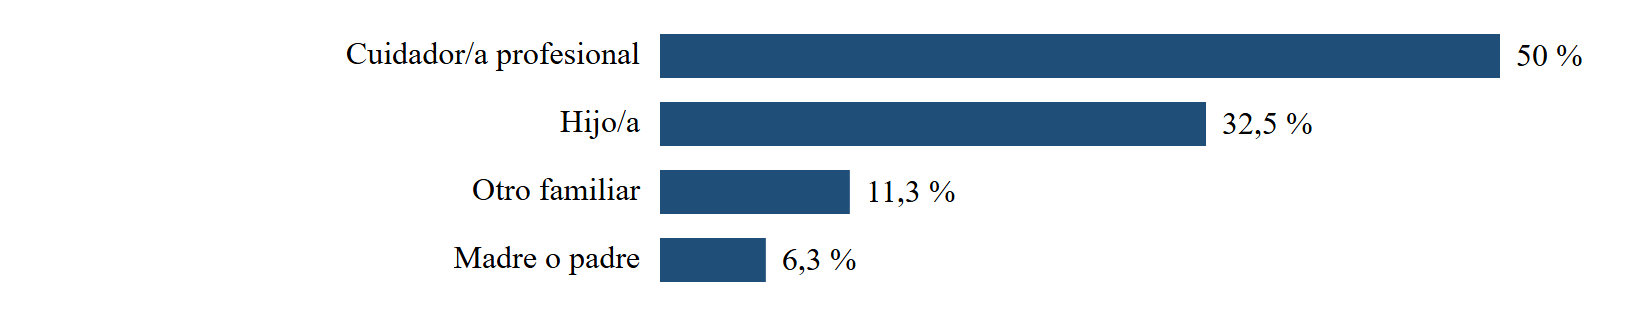
\includegraphics[width=\textwidth]{figuras/fig-7-1}
\caption{Relación con la persona que cuida (estudio simulado, 80 casos)}\label{fig:fig-7-1}
\end{figure}

{\small
\begin{xltabular}{\textwidth}{>{\raggedright\arraybackslash}X >{\raggedright\arraybackslash}X l}
\caption{Perfil de los casos del estudio simulado}\label{tab:c7-1}\\
\toprule
\tb{Pregunta} & \tb{Respuesta} & \tb{Casos} \\
\midrule
\endfirsthead
\toprule
\tb{Pregunta} & \tb{Respuesta} & \tb{Casos} \\
\midrule
\endhead
\bottomrule
\endfoot
Tiempo que lleva cuidando & Menos de 1 año & 17,5~\% \\
 & Entre 1 y 3 años & 57,5~\% \\
 & Entre 4 y 7 años & 3,8~\% \\
 & Más de 7 años & 21,3~\% \\
Horas por día dedicadas al cuidado & Menos de 4 horas & 25,0~\% \\
 & Entre 4 y 8 horas & 60,0~\% \\
 & Entre 8 y 12 horas & 7,5~\% \\
 & Más de 12 horas & 7,5~\% \\
Tipo de discapacidad de la persona & Motora & 32,5~\% \\
 & Intelectual & 27,5~\% \\
 & Autismo (TEA) & 20,0~\% \\
 & Visual & 15,0~\% \\
 & Múltiple & 5,0~\% \\
\end{xltabular}
}

\subsection{Organizar la información del cuidado}

Al 57,5~\% le resulta difícil o muy difícil organizar la información relacionada con el cuidado, como los turnos, la medicación, los estudios o los certificados. Solo al 2,5~\% le resulta fácil. El nivel de estrés que genera esa organización se ubica en un punto intermedio para la mayoría, con un promedio de 2,9 sobre 5, y el 76,3~\% lo califica como moderado.

\begin{figure}[H]
\centering
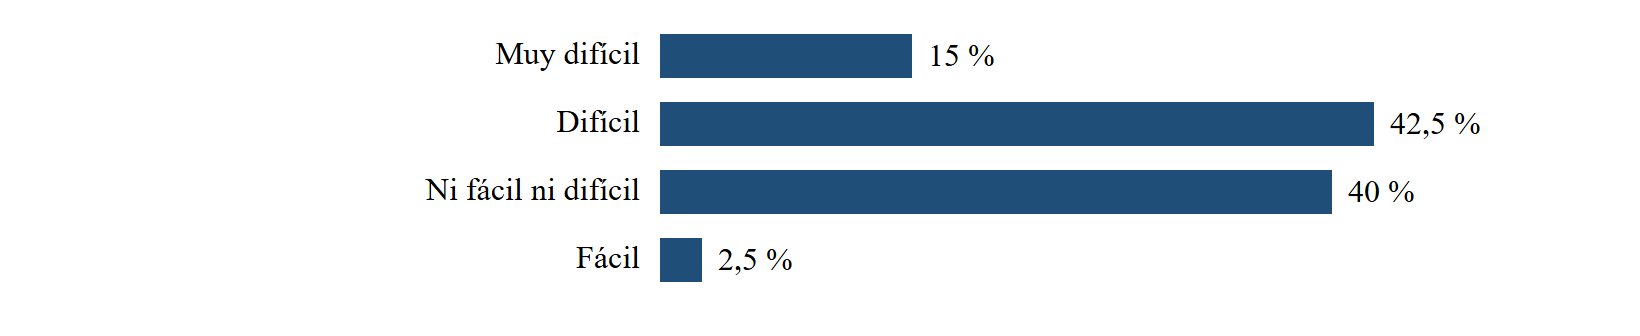
\includegraphics[width=\textwidth]{figuras/fig-7-2}
\caption{Dificultad para organizar la información del cuidado}\label{fig:fig-7-2}
\end{figure}

Entre los problemas más frecuentes se destaca sentirse acompañado o recibir orientación, que mencionan dos de cada tres casos. Le siguen coordinar tareas con otros cuidadores, controlar la medicación, encontrar información confiable y recordar los turnos médicos.

\begin{figure}[H]
\centering
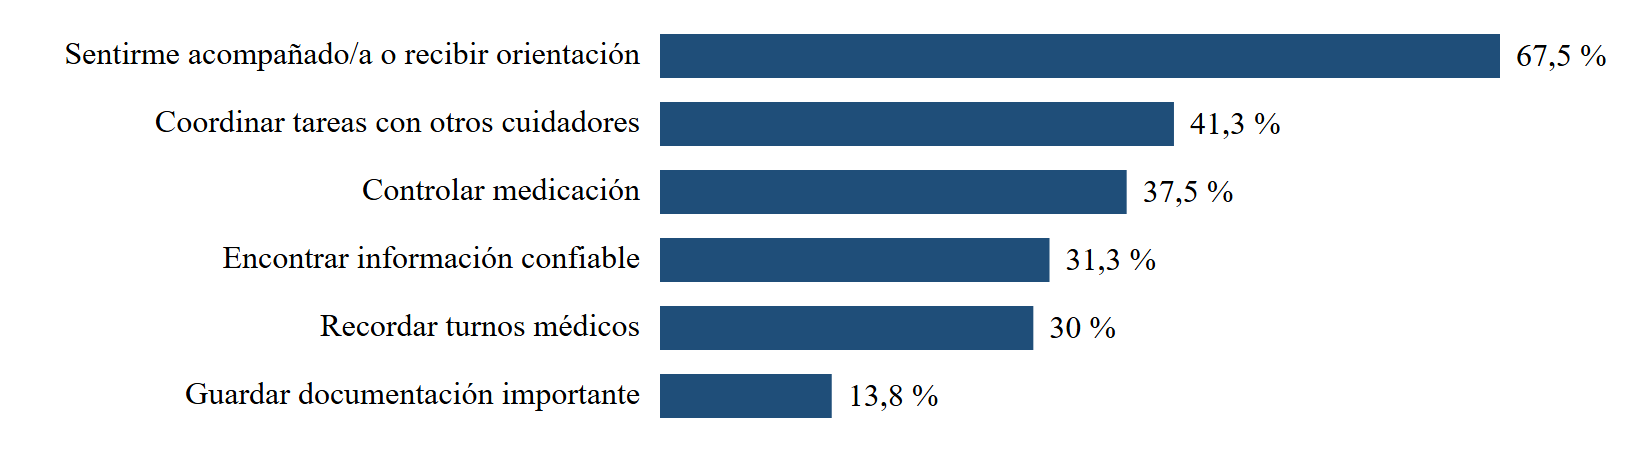
\includegraphics[width=\textwidth]{figuras/fig-7-3}
\caption{Problemas más frecuentes (respuesta múltiple)}\label{fig:fig-7-3}
\end{figure}

La dificultad para coordinar con otros cuidadores aparece sobre todo entre quienes cuidan de forma profesional. La señala el 62,5~\% de los cuidadores profesionales, frente al 20~\% de los familiares.

\subsection{Herramientas que se usan hoy}

La agenda en papel es la herramienta más usada, por el 87,5~\% de los casos, seguida por el calendario del celular, con un 62,5~\%, y por WhatsApp, con un 36,3~\%. El 71,3~\% combina dos herramientas o más, lo que muestra que la información del cuidado está repartida entre varios lugares. Solo el 2,5~\% no usa ninguna.

\begin{figure}[H]
\centering
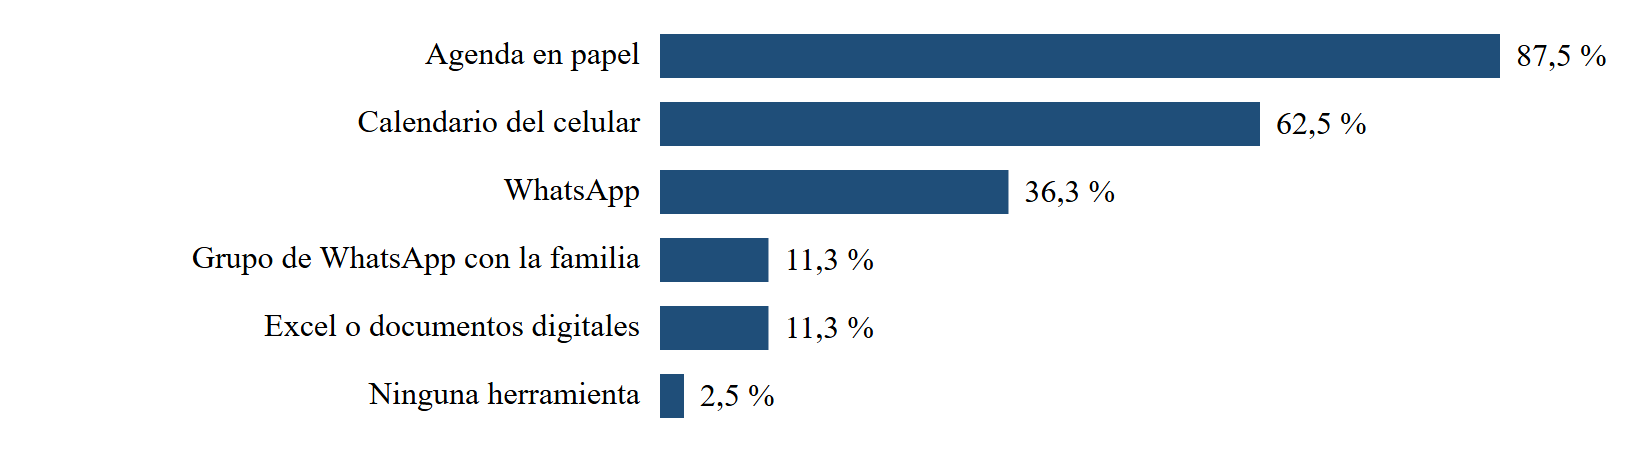
\includegraphics[width=\textwidth]{figuras/fig-7-4}
\caption{Herramientas que se usan hoy para organizar el cuidado (respuesta múltiple)}\label{fig:fig-7-4}
\end{figure}

\subsection{Interés en una herramienta como la propuesta}

El 80~\% considera que una herramienta como la propuesta le resultaría muy o bastante útil, y nadie respondió que no le serviría. El 61,3~\% afirma que usaría una aplicación web o móvil para gestionar el cuidado y el 38,8~\% no está seguro, mientras que ningún caso respondió que no la usaría. En la pregunta abierta, lo que más ayudaría hoy es tener resuelta la medicación y las rutinas, mejorar el acceso al sistema de salud, tener la información en un solo lugar y conseguir turnos con más facilidad.

\begin{figure}[H]
\centering

\includegraphics[width=\textwidth]{figuras/fig-7-5}
\caption{¿Una herramienta así le sería útil?}\label{fig:fig-7-5}
\end{figure}

\subsection{Qué decisiones de diseño se tomaron a partir del relevamiento}

\begin{table}[H]
\centering
\caption{Hallazgos del relevamiento y respuesta del sistema}\label{tab:c7-2}
\small
\begin{tabularx}{\textwidth}{>{\raggedright\arraybackslash}X >{\raggedright\arraybackslash}X}
\toprule
\tb{Hallazgo} & \tb{Cómo lo responde el sistema} \\
\midrule
La mitad de los casos son cuidadores profesionales y les cuesta coordinar con otros. & Grupos de cuidado con dueño, cuidadores y observadores, cada uno con su cuenta, y el registro de quién hizo cada cosa. \\
Dos de cada tres no se sienten acompañados ni orientados. & Guía de trámites, recursos y artículos según la discapacidad de la persona, y la sección Tu bienestar con líneas de ayuda. \\
La información está en la agenda de papel, el celular y WhatsApp. & Tu día reúne turnos y medicación en un solo lugar, con la ficha y los documentos de cada persona. \\
Controlar la medicación y recordar los turnos son problemas frecuentes. & Agenda de tomas con quién dio cada una, avisos de tomas atrasadas, recetas por vencer y controles que se repiten. \\
Encontrar información confiable cuesta. & Cada recurso y cada paso de la guía de trámites enlaza a su fuente oficial, y cada recomendación explica por qué aparece. \\
\bottomrule
\end{tabularx}
\end{table}

\section{Punto de partida}

Al comenzar esta etapa, el proyecto contaba con un prototipo de interfaz, una aplicación web autocontenida, sin servidor, con datos ficticios escritos directamente en el código y con un motor de recomendación que solo mostraba puntajes de ejemplo. Se habían fijado cuatro pasos siguientes. Implementar la API REST y el modelo de datos, migrar la interfaz a React con Vite, desarrollar una primera versión del motor de recomendación y validar la plataforma con usuarios.

Los tres primeros pasos se completaron. La plataforma pasó a ser un sistema funcional, con persistencia en base de datos, autenticación real, control de accesos por usuario y un motor de recomendación que calcula sus resultados a partir del perfil de cada persona asistida. Además, el motor incorporó la valoración de los cuidadores, con lo que pasó a funcionar como un sistema híbrido.

A partir de la revisión del sistema con el director del proyecto, el alcance se ajustó. Se retiraron la comunidad de cuidadores y el rol de especialista, y en su lugar se incorporó una sección de artículos ya publicados por especialistas, seleccionados y con enlace a su fuente. Se agregaron los grupos de cuidado, en los que el dueño de una cuenta ya sea una familia o una institución, suma cuidadores y observadores con su propia cuenta, y un modelo de tres planes con una base gratuita. Más adelante, los recursos y los artículos pasaron a mostrarse según el tipo de discapacidad de cada persona.

\section{Requisitos funcionales y estado de cumplimiento}

{\small
\begin{xltabular}{\textwidth}{l >{\raggedright\arraybackslash}X l >{\raggedright\arraybackslash}X}
\caption{Requisitos funcionales y estado de cumplimiento}\label{tab:rf}\\
\toprule
\tb{ID} & \tb{Requisito} & \tb{Estado} & \tb{Observaciones} \\
\midrule
\endfirsthead
\toprule
\tb{ID} & \tb{Requisito} & \tb{Estado} & \tb{Observaciones} \\
\midrule
\endhead
\bottomrule
\endfoot
RF01 & Registro, inicio de sesión y recuperación de contraseña por correo. & Cumplido & Un solo tipo de cuenta. Quien se registra es dueño de su grupo. \\
RF02 & Alta, edición y baja de personas asistidas con su perfil (tipo de discapacidad, obra social, localidad, necesidades). & Cumplido & El tipo de discapacidad es obligatorio, porque define recursos, artículos y estudios. \\
RF03 & Grupo de cuidado con cuidadores y observadores, cada uno con su cuenta. & Cumplido & El dueño suma integrantes con su correo y elige a qué personas acompaña cada uno. El cuidador registra y el observador solo mira. \\
RF04 & Seguimiento del grupo por persona y por cuidador. & Cumplido & Todo lo registrado con su autor, tomas sin registrar y, con el plan Plus, el cumplimiento de cada cuidador. \\
RF05 & Planes Básico, Intermedio y Plus con sus límites. & Parcial & Los límites se controlan en la API y en la interfaz. El pago está simulado, sin pasarela real. \\
RF06 & Agenda de turnos médicos con vista de calendario y controles que se repiten. & Cumplido & Vista mensual, próximos turnos y aviso un mes antes de cada control periódico. \\
RF07 & Registro de medicación con agenda diaria de tomas. & Cumplido & Se registra quién dio cada toma y se avisan recetas por vencer. \\
RF08 & Carga, búsqueda y descarga de documentos (estudios, recetas, certificados). & Cumplido & Con validación del tipo real de archivo y espacio según el plan. \\
RF09 & Módulo de emergencia con acceso al SAME (107) y a la red de apoyo. & Cumplido & Disponible en todos los planes. El llamado se resuelve con un enlace telefónico directo. \\
RF10 & Ficha de emergencia imprimible por persona. & Cumplido & Grupo sanguíneo, alergias, diagnóstico, médico y obra social. \\
RF11 & Guía de trámites según el tipo de discapacidad, con seguimiento del avance. & Cumplido & Basada en normativa oficial. Cada paso indica su fuente. \\
RF12 & Recursos específicos de la discapacidad de la persona, ordenados por relevancia y explicados. & Cumplido & Cada tarjeta muestra por qué se recomienda. \\
RF13 & Valoración de los recursos por parte del cuidador (``me sirvió'' / ``no me sirvió''). & Cumplido & Alimenta la parte colaborativa del recomendador. \\
RF14 & Artículos de especialistas por tipo de discapacidad y generales sobre el cuidado. & Cumplido & 20 artículos ya publicados, cada uno con su fuente y su enlace. \\
RF15 & Diario de cuidado con resumen imprimible para la consulta médica. & Cumplido & Incluye la medicación actual, las tomas que se dieron y las que no. \\
RF16 & Autoevaluación del esfuerzo del cuidador con orientación y líneas de ayuda. & Cumplido & Índice de Esfuerzo del Cuidador (13 preguntas). \\
RF17 & Administración de recursos y artículos. & Cumplido & Alta, edición y baja, con uno o más tipos de discapacidad por recurso. No se revisó en el navegador en esta instancia. \\
\end{xltabular}
}

De los 17 requisitos, 16 se cumplieron por completo y 1 de forma parcial.

La tabla~\ref{tab:rf-criterios} define la prioridad y el criterio de aceptación de cada requisito, y lo vincula con el indicador del capítulo~\ref{cap:metodologia} al que aporta.

{\small
\begin{xltabular}{\textwidth}{l l >{\raggedright\arraybackslash}X >{\raggedright\arraybackslash}p{3.2cm}}
\caption{Prioridad, criterio de aceptación e indicador de cada requisito funcional}\label{tab:rf-criterios}\\
\toprule
\tb{ID} & \tb{Prioridad} & \tb{Criterio de aceptación} & \tb{Indicador} \\
\midrule
\endfirsthead
\toprule
\tb{ID} & \tb{Prioridad} & \tb{Criterio de aceptación} & \tb{Indicador} \\
\midrule
\endhead
\bottomrule
\endfoot
RF01 & Alta & Una cuenta nueva se registra, inicia sesión y recupera la contraseña por correo sin intervención manual. & Facilidad de uso \\
RF02 & Alta & Una persona se crea, edita y borra, y al borrarla se eliminan todos sus registros. & Facilidad de uso \\
RF03 & Alta & Un observador recibe un error al intentar registrar y un cuidador solo ve a las personas que tiene asignadas. & Percepción de apoyo \\
RF04 & Media & El dueño ve el autor de cada registro y las tomas sin registrar de los últimos 7 días. & Percepción de apoyo \\
RF05 & Media & Una cuenta del plan Básico no puede crear una segunda persona ni abrir secciones de otros planes. & Intención de uso \\
RF06 & Alta & Un control que se repite genera un aviso 30 días antes del próximo turno. & Utilidad percibida \\
RF07 & Alta & Cada toma guarda quién la registró y a qué hora, y se avisa la receta próxima a vencer. & Utilidad percibida \\
RF08 & Media & Se rechaza un archivo cuyo contenido no coincide con su extensión y se respeta el espacio del plan. & Facilidad de uso \\
RF09 & Alta & El acceso al 107 está visible en todas las pantallas y en todos los planes. & Percepción de apoyo \\
RF10 & Media & La ficha impresa incluye grupo sanguíneo, alergias, diagnóstico, médico y obra social. & Utilidad percibida \\
RF11 & Alta & Cada paso de la guía muestra su fuente oficial y el avance se guarda por persona. & Utilidad percibida \\
RF12 & Alta & El 100~\% de las recomendaciones tiene explicación y todas son del tipo de discapacidad de la persona. & Recomendaciones explicadas \\
RF13 & Media & Una valoración cambia el orden de las recomendaciones de personas con la misma discapacidad. & Precisión del recomendador \\
RF14 & Media & Cada artículo tiene fuente y enlace verificado, con al menos uno por tipo de discapacidad. & Cobertura del catálogo \\
RF15 & Media & El resumen imprimible incluye la medicación actual y las tomas dadas y no dadas. & Utilidad percibida \\
RF16 & Baja & El cuestionario de 13 preguntas calcula el resultado y muestra orientación y líneas de ayuda. & Percepción de apoyo \\
RF17 & Baja & Una cuenta de administración crea, edita y desactiva recursos y artículos. & Cobertura del catálogo \\
\end{xltabular}
}

\section{Requisitos no funcionales y evidencia obtenida}

\begin{table}[H]
\centering
\caption{Requisitos no funcionales y evidencia obtenida}\label{tab:rnf}
\footnotesize
\begin{tabularx}{\textwidth}{l >{\raggedright\arraybackslash}X >{\raggedright\arraybackslash}X >{\raggedright\arraybackslash}X}
\toprule
\tb{ID} & \tb{Requisito} & \tb{Evidencia} & \tb{Estado} \\
\midrule
RNF01 & Usabilidad y accesibilidad & Tipografía de alta legibilidad, tres tamaños de letra, modo de alto contraste, foco visible al navegar con teclado y textos en lenguaje claro. & Cumplido a nivel técnico, falta validar con usuarios \\
RNF02 & Diseño adaptable a celulares & Las doce pantallas se revisaron a 375 px de ancho, sin desplazamiento horizontal. En celulares la navegación pasa a una barra inferior. & Cumplido \\
RNF03 & Seguridad de acceso & Contraseñas con hash, token firmado, roles, bloqueo de la cuenta durante 5 minutos tras 5 intentos fallidos y filtrado de los datos por persona asistida. & Cumplido \\
RNF04 & Privacidad entre grupos & Cada usuario ve solo sus personas y las de los grupos donde ayuda. Cada cuidador ve solo a quienes tiene asignados y nadie ve el grupo de otro dueño, cubierto por pruebas automatizadas. & Cumplido \\
RNF05 & Tiempo de respuesta & Mediana de 6,8 ms y percentil 95 de 9,2 ms al calcular recomendaciones. & Cumplido (medido en el entorno local) \\
RNF06 & Mantenibilidad & 18 migraciones versionadas del esquema, 68 pruebas automatizadas, separación en capas y código en un repositorio con control de versiones. & Cumplido \\
RNF07 & Disponibilidad en la nube & Todavía no se publicó. El sistema se ejecuta en un entorno local y la publicación en Azure App Service y Azure SQL Database queda como próximo paso. & Pendiente \\
\bottomrule
\end{tabularx}
\end{table}

\begin{table}[H]
\centering
\caption{Prioridad y criterio de aceptación de cada requisito no funcional}\label{tab:rnf-criterios}
\small
\begin{tabularx}{\textwidth}{l l >{\raggedright\arraybackslash}X}
\toprule
\tb{ID} & \tb{Prioridad} & \tb{Criterio de aceptación} \\
\midrule
RNF01 & Alta & Todas las pantallas se recorren con teclado y el texto admite tres tamaños sin perder información. \\
RNF02 & Alta & Ninguna pantalla genera desplazamiento horizontal a 375 px de ancho. \\
RNF03 & Alta & Las contraseñas se guardan con hash y la cuenta se bloquea tras 5 intentos fallidos. \\
RNF04 & Alta & Ninguna prueba automatizada de acceso entre grupos permite ver o modificar datos ajenos. \\
RNF05 & Media & El cálculo de recomendaciones responde en menos de 1 segundo en el percentil 95. \\
RNF06 & Media & El esquema se reproduce con las migraciones y las pruebas se ejecutan con un solo comando. \\
RNF07 & Media & El sistema es accesible públicamente por HTTPS. \\
\bottomrule
\end{tabularx}
\end{table}

\section{Arquitectura implementada}

Se respetó la arquitectura en capas descripta en el Capítulo 4, una interfaz web en React, una API REST en ASP.NET Core que contiene la lógica de negocio y el motor de recomendación, y una base de datos relacional en SQL Server.

\begin{table}[H]
\centering
\caption{Diferencias entre la arquitectura planificada y la implementada}\label{tab:c7-5}
\footnotesize
\begin{tabularx}{\textwidth}{>{\raggedright\arraybackslash}X >{\raggedright\arraybackslash}X >{\raggedright\arraybackslash}X}
\toprule
\tb{Aspecto} & \tb{Planificado} & \tb{Implementado y motivo} \\
\midrule
Control de acceso a los datos & Row-Level Security de SQL Server. & Un único servicio de la API decide, para cada persona asistida, si el usuario puede verla, registrar en ella o administrarla, y todos los controladores lo usan. Se eligió así para poder probarlo con pruebas automatizadas. \\
Cifrado en reposo & Transparent Data Encryption en Azure SQL. & Pendiente. Se activará al publicar en Azure SQL Database, que aplica Transparent Data Encryption por defecto. Hoy se usa SQL Server Express en el entorno local, solo con datos de demostración. \\
Conexión con el SAME & API de emergencias del SAME. & Enlace telefónico directo al 107 visible desde todas las pantallas. No existe una API pública, como se previó en el riesgo R7. \\
Motor de recomendación & Basado en contenido en la primera versión. & Híbrido. Perfil de la persona más valoraciones de los cuidadores. \\
Cobro de los planes & Pasarela de pagos. & Cambio de plan simulado desde la cuenta. Los límites de cada plan sí se aplican en la API. \\
Sesión del usuario & Token emitido por la API. & Token JWT guardado en el navegador. Es aceptable para un prototipo, pero una cookie protegida reduciría el riesgo ante ataques de inyección de código. \\
Cuentas & Cuentas de familia y de institución por separado. & Un solo tipo de cuenta. Una institución es el dueño de un grupo con plan Plus, lo que simplifica el modelo y sirve igual para una familia grande. \\
\bottomrule
\end{tabularx}
\end{table}

\section{Modelo de datos}

El modelo de datos quedó compuesto por 14 entidades propias, además de las tablas de usuarios y roles que provee ASP.NET Core Identity. Pueden agruparse en cinco bloques. La persona asistida y su cuidado diario (turnos, medicamentos, tomas, diario y documentos), la emergencia (contactos y ficha, incluida en la persona), la orientación (recursos, valoraciones de recursos, avance de trámites y artículos), la organización del cuidado (los integrantes de cada grupo) y el bienestar del cuidador (evaluaciones de esfuerzo).

Cada persona asistida tiene un responsable, que es el dueño del grupo. Los integrantes se resuelven con una tabla que vincula a la persona con cada usuario y su rol, cuidador u observador, sin modificar quién es el dueño. El plan y el nombre del grupo se guardan en la cuenta del dueño, y el plan que cubre a cada persona es siempre el de su dueño.

Las relaciones se definieron con claves foráneas y, en los casos que corresponde, con borrado en cascada. Al eliminar una persona asistida se eliminan sus turnos, medicamentos, documentos, valoraciones, avances de trámites e integrantes del grupo. Para evitar registros duplicados se agregaron índices únicos, por ejemplo, una sola valoración por persona y recurso, y una sola toma por medicamento, día y horario.

\section{Diseño de la interfaz}

El diseño de la interfaz siguió los principios de la norma ISO 9241-210 \citep{une2019}. Se adoptó la tipografía Atkinson Hyperlegible, desarrollada por el Braille Institute para personas con baja visión, y se limitó el uso del color a lo que transmite información, un color de acento para lo que requiere atención, rojo solo para la emergencia y un color distinto por cada persona asistida, de modo que en el calendario o en la medicación se reconozca a quién corresponde cada registro.

La pantalla de inicio se organizó como una línea del día, que reúne en orden horario los turnos y las tomas de medicación y permite registrar una toma sin cambiar de sección. El menú agrupa las secciones según para qué se usan. Cuidado diario reúne lo que se registra de cada persona, Orientación lo que se consulta para saber qué hacer, Quienes cuidan el grupo y el bienestar de quien cuida, y Cuenta el plan. La interfaz se adapta a lo que cada persona puede hacer. A un observador no se le muestran los botones para registrar, a la dueña de una residencia se le muestra el estado de cada toma y a cargo de quién está, y lo que no incluye el plan aparece con una explicación de qué plan lo incluye.

\section{Construcción e integración}

El código fuente completo está disponible en el repositorio descripto en el anexo~\ref{anx:repositorios}, y el apéndice~B explica cómo ejecutarlo en un entorno local. Su publicación en Azure queda como próximo paso.

El desarrollo se realizó de forma incremental. Cada módulo se construyó primero en la API, con su entidad y su migración, luego se integró en la interfaz y por último se probó de punta a punta.

\begin{table}[H]
\centering
\caption{Dimensiones del sistema construido}\label{tab:c7-6}
\small
\begin{tabularx}{\textwidth}{>{\raggedright\arraybackslash}X >{\raggedright\arraybackslash}X}
\toprule
\tb{Indicador} & \tb{Valor} \\
\midrule
Endpoints de la API & 68, distribuidos en 14 controladores \\
Entidades del modelo de datos & 14 (más las de Identity) \\
Migraciones del esquema & 18 \\
Vistas de la interfaz & 13 \\
Líneas de código del backend (sin migraciones) & 7.358 \\
Líneas de código del frontend (JavaScript y JSX) & 7.946 \\
Líneas de hojas de estilo & 5.528 \\
Líneas de código de pruebas automatizadas & 896 \\
\bottomrule
\end{tabularx}
\end{table}

Para probar el sistema en condiciones parecidas a las reales se cargó un conjunto de datos de demostración. Ocho familias con distintos planes y nueve personas asistidas de distintos tipos de discapacidad, obras sociales y localidades, una cuidadora contratada que atiende a personas de dos familias, una familiar en modo observador, y una residencia con su dueña, dos cuidadores y cuatro residentes. Al iniciar, el sistema completa la última semana de tomas y corre el diario de prueba, para que la demostración refleje siempre días recientes. Todos los datos son ficticios. El código se guarda en un repositorio privado con control de versiones.

\section{Motor de recomendación}

El motor se implementó como un servicio interno de la API, sin librerías externas de aprendizaje automático. Cada recurso del catálogo corresponde a uno o más tipos de discapacidad, y el motor solo considera los del tipo de la persona. Lo que sirve a cualquier persona, como el CUD, la pensión o el transporte, está en la guía de trámites. Para cada recurso del tipo de la persona sigue tres pasos. Primero descarta los que piden algo que la persona no cumple, un recurso de PAMI no se muestra a quien tiene otra obra social, ni uno de Rosario a alguien de Escobar, y uno marcado como ``sin obra social'' no se muestra a quien tiene una. Después suma puntos por cada coincidencia entre el perfil y el recurso. Por último, ajusta el orden según las valoraciones.

\begin{table}[H]
\centering
\caption{Pesos utilizados por el motor de recomendación}\label{tab:c7-7}
\small
\begin{tabularx}{\textwidth}{>{\raggedright\arraybackslash}X l >{\raggedright\arraybackslash}X}
\toprule
\tb{Criterio} & \tb{Puntos} & \tb{Cuándo se aplica} \\
\midrule
Tipo de discapacidad & 40 & El recurso es para el tipo de discapacidad de la persona. Es condición para que aparezca. \\
Necesidades & 35 & El recurso responde a al menos una de las necesidades marcadas en el perfil. \\
Obra social & 30 & El recurso es de la obra social de la persona. \\
Localidad & 30 & El recurso está en la localidad de la persona. \\
Valoración propia positiva & +30 & Quien cuida a la persona marcó ``me sirvió''. \\
Valoración propia negativa & al final & Quien cuida marcó ``no me sirvió''. El recurso pasa al final de la lista, sin desaparecer. \\
Valoraciones de otros cuidadores & hasta $\pm$20 & Votos de cuidadores de personas con el mismo tipo de discapacidad. Con menos de tres votos el ajuste se reduce en proporción. \\
\bottomrule
\end{tabularx}
\end{table}

El porcentaje de coincidencia que ve el usuario se calcula solo con los puntos del perfil, sobre un máximo de 135. Las valoraciones modifican el orden, pero no ese porcentaje, para que el número siga expresando cuánto se ajusta el recurso a la situación de la persona. Cada criterio que suma puntos genera una explicación, y cuando un recurso sube por las valoraciones de otros se indica a cuántos cuidadores les sirvió.

La parte colaborativa compara solamente con personas del mismo tipo de discapacidad, de modo que una valoración sobre un recurso para personas con discapacidad motora no influye en lo que se le muestra a una familia que cuida a alguien con discapacidad visual. Con esto se atiende el problema del arranque en frío descripto en el Capítulo 3, ya que mientras no haya valoraciones el sistema funciona igual que uno basado en contenido.

\section{Contenido de orientación}\label{sec:contenido}

La guía de trámites se armó a partir de las normativas oficiales de certificación de la discapacidad (Disposiciones del Servicio Nacional de Rehabilitación 1019, 639, 82, 648 y 500 de 2015) y de páginas oficiales de argentina.gob.ar, la Superintendencia de Servicios de Salud, la CNRT y ANSES. Se organiza en cuatro etapas. La consulta de requisitos del CUD, los estudios que corresponden según el tipo de discapacidad, la presentación ante la junta evaluadora y los derechos a los que se accede con el certificado. Cada paso indica su fuente y su enlace, y una prueba automatizada verifica que ninguno quede sin fuente.

El catálogo de recursos recomendables quedó integrado por 20 recursos activos, todos de uno o más tipos de discapacidad. Diez son de alcance nacional y diez son locales, ubicados en Pilar, la Ciudad de Buenos Aires, Córdoba, La Plata, Rosario, Escobar, Tigre y San Isidro. La sección de artículos reúne 20 textos ya publicados, seis generales sobre el cuidado y catorce de un tipo de discapacidad, de modo que cada tipo tiene al menos uno. Provienen de materiales oficiales para cuidadores, de la Organización Mundial de la Salud y la Organización Panamericana de la Salud, y de revistas científicas, y cada uno lleva a su fuente original.

\section{Pruebas automatizadas}

Se desarrolló un proyecto de pruebas con xUnit que utiliza una base de datos SQLite en memoria, de manera que cada prueba trabaja sobre datos propios y no depende de la base real. Las pruebas se concentraron en las partes donde un error tendría consecuencias más graves, el acceso a datos de terceros, los permisos dentro de los grupos, los límites de los planes, el cálculo de las recomendaciones, la guía de trámites y la escala de esfuerzo.

\begin{table}[H]
\centering
\caption{Pruebas automatizadas por área}\label{tab:c7-8}
\footnotesize
\begin{tabularx}{\textwidth}{>{\raggedright\arraybackslash}X >{\raggedright\arraybackslash}X l l}
\toprule
\tb{Clase de prueba} & \tb{Qué verifica} & \tb{Casos} & \tb{Ok} \\
\midrule
AccesoCompartidoTests & Que cada usuario vea solo sus personas y las de su grupo, que alguien ajeno no pueda modificar la medicación y que al borrar una persona se borre todo lo suyo. & 8 & 8 \\
EquipoYPlanesTests & Que el observador vea sin registrar, que el cuidador registre sin administrar, que cada cuidador vea solo a sus asignados y quede cubierto por el plan del dueño, que nadie vea el grupo de otro, lo que el dueño ve de cada uno y los límites de cada plan. & 16 & 16 \\
RecomendacionServiceTests & El orden por coincidencia, que solo aparezcan recursos del tipo de la persona, el descarte por localidad y por ``sin obra social'', la tolerancia a mayúsculas y tildes, el tope del porcentaje y el efecto de las valoraciones. & 10 & 10 \\
GuiaTramitesTests & Que cada tipo de discapacidad vea solo sus estudios, los pasos según la edad y el parentesco, y que todos los pasos tengan fuente y enlace oficial. & 15 & 15 \\
EscalaEsfuerzoTests & Las 13 preguntas del índice, el punto de corte en 7 respuestas afirmativas y las sugerencias derivadas. & 5 & 5 \\
FormatoTests & Horarios de medicación válidos e inválidos, el nombre que se muestra sin título profesional y la regla de las cuentas de demostración. & 14 & 14 \\
\textbf{Total} &  & \textbf{68} & \textbf{68} \\
\bottomrule
\end{tabularx}
\end{table}

Las 68 pruebas se ejecutaron con resultado satisfactorio. Además, la compilación del backend no registra advertencias y el análisis estático del frontend no informa errores.

\section{Pruebas de integración}

Las pruebas de integración se realizaron contra la API en ejecución y desde el navegador, recorriendo los flujos completos. Registro e inicio de sesión, alta y edición de una persona, cálculo de recomendaciones, carga de turnos, subida de un documento válido y rechazo de un archivo con extensión falsa, descarga, registro de tomas y valoración de recursos. Para los grupos se verificó sumar a una observadora y quitarla, cambiar a quiénes acompaña un cuidador, que un observador reciba un error de permiso al intentar registrar una toma y que cada plan habilite solo lo que le corresponde. También se probó el aviso de un control que se repite con un turno de prueba. Los datos creados para estas pruebas se eliminaron al finalizar.

\section{Pruebas de interfaz y accesibilidad}\label{sec:interfaz}

La interfaz se revisó en pantallas de computadora y a 375 px de ancho, equivalente a un celular, con cuentas de distintos roles, la dueña de una residencia, una familia con cada uno de los tres planes, una cuidadora contratada y una observadora. Se comprobó que cada rol vea solo las acciones que le corresponden y que ninguna de las doce pantallas genere desplazamiento horizontal. También se revisaron la combinación de letra muy grande con alto contraste y la navegación con teclado.

\section{Rendimiento}

Se midió el tiempo de respuesta del cálculo de recomendaciones, que es la operación más costosa del sistema porque recorre el catálogo y las valoraciones. Se tomaron 65 mediciones, cinco por cada una de las trece personas evaluadas, en el equipo de desarrollo y descartando la primera llamada de cada persona.

\begin{table}[H]
\centering
\caption{Tiempo de respuesta del cálculo de recomendaciones}\label{tab:c7-9}
\small
\begin{tabularx}{\textwidth}{l l}
\toprule
\tb{Medida} & \tb{Valor} \\
\midrule
Mediciones & 65 \\
Promedio & 7,1 ms \\
Mediana & 6,8 ms \\
Percentil 95 & 9,2 ms \\
Máximo & 9,9 ms \\
\bottomrule
\end{tabularx}
\end{table}

Los tiempos son bajos para el volumen actual, pero se midieron en el entorno local de desarrollo, con un catálogo de 20 recursos. No permiten anticipar el comportamiento con miles de recursos ni con muchos usuarios simultáneos una vez publicado en Azure.

\section{Seguimiento del grupo con los datos de demostración}\label{sec:seguimiento}

Para comprobar que el panel del grupo permite detectar diferencias en el trabajo de cada cuidador, se usaron los registros de la última semana de la residencia de demostración. Una cuidadora registra todas las tomas a tiempo y el otro deja tomas sin registrar y anota tarde. El panel mostró los resultados que se esperaban a partir de esos datos.

\begin{table}[H]
\centering
\caption{Indicadores del panel del grupo (últimos 7 días)}\label{tab:c7-10}
\small
\begin{tabularx}{\textwidth}{l >{\raggedright\arraybackslash}X l >{\raggedright\arraybackslash}X >{\raggedright\arraybackslash}X}
\toprule
\tb{Cuidador} & \tb{Tomas registradas} & \tb{Sin registrar} & \tb{Registradas tarde} & \tb{Entradas del diario} \\
\midrule
Carla Ruiz & 100~\% (39 de 39) & 0 & 0 & 3 \\
Diego Paredes & 70~\% (28 de 40) & 12 & 28 & 1 \\
\bottomrule
\end{tabularx}
\end{table}

Este resultado solo muestra que el panel calcula y presenta correctamente los indicadores. Si le resulta útil a una institución real, y si los indicadores se interpretan de manera adecuada, deberá evaluarse con instituciones, como se advierte en el riesgo R11.

\section{Defectos encontrados}

Durante las pruebas se registraron los siguientes defectos. Todos se corrigieron.

{\small
\begin{xltabular}{\textwidth}{l >{\raggedright\arraybackslash}X >{\raggedright\arraybackslash}X l}
\caption{Defectos detectados durante las pruebas}\label{tab:c7-11}\\
\toprule
\tb{ID} & \tb{Defecto} & \tb{Cómo se detectó} & \tb{Estado} \\
\midrule
\endfirsthead
\toprule
\tb{ID} & \tb{Defecto} & \tb{Cómo se detectó} & \tb{Estado} \\
\midrule
\endhead
\bottomrule
\endfoot
D1 & En celulares, el calendario mensual excedía el ancho de la pantalla (486 px de contenido en 375 px). & Revisión de interfaz en 375 px & Corregido \\
D2 & El menú ``Más'' del celular no se cerraba con la tecla Escape ni llevaba el foco al menú. & Prueba con teclado & Corregido \\
D3 & En pantallas angostas, los contactos de emergencia propios quedaban debajo de los números generales, fuera de la vista. & Observación de uso & Corregido \\
D4 & Cuatro recursos enlazaban a páginas inexistentes (error 404). & Revisión de enlaces & Corregido \\
D5 & Trece recursos enlazaban a portadas genéricas en lugar de la página del tema descripto. & Revisión de enlaces & Corregido \\
D6 & Tres recursos estaban duplicados por una versión anterior de los datos iniciales. & Revisión de la base de datos & Corregido \\
D7 & En celulares, el encabezado de la ficha de una persona excedía el ancho de la pantalla. & Revisión de interfaz en ancho de celular & Corregido \\
D8 & Una fila de filtros no pasaba a una segunda línea en pantallas angostas. & Revisión de interfaz en ancho de celular & Corregido \\
D9 & En la pantalla de planes, el precio del plan Básico aparecía repetido. & Revisión de interfaz & Corregido \\
D10 & El programa Incluir Salud se recomienda a personas afiliadas a PAMI, aunque solo corresponde a titulares de pensiones no contributivas sin obra social. & Evaluación del recomendador & Corregido \\
D11 & Algunos perfiles no reciben ningún recurso local ni específico de su discapacidad. & Evaluación del recomendador & Corregido \\
D12 & La sección Tu bienestar sugería ir a la comunidad de cuidadores, que ya no existía. & Revisión de contenido & Corregido \\
D13 & La página de ANSES de la pensión no contributiva no respondía. Se reemplazó por la página oficial de argentina.gob.ar. & Revisión de enlaces & Corregido \\
D14 & El aviso de controles que se repiten no aparecía porque la fecha del próximo control se calculaba mal. & Prueba con un turno de prueba & Corregido \\
\end{xltabular}
}

El defecto D10 se resolvió agregando al motor la condición ``sin obra social'', que deja un recurso solo para quien no tiene obra social o se atiende por Incluir Salud. El D11 se resolvió ampliando el catálogo con recursos reales en Escobar, Tigre y San Isidro y con recursos específicos para discapacidad visceral, visual y múltiple.

\section{Evaluación del motor de recomendación}\label{sec:eval-motor}

Para evaluar el motor se calcularon las recomendaciones de las trece personas asistidas de demostración, sobre el catálogo de 20 recursos. La tabla muestra, para cada perfil, cuántos recursos se recomendaron, cuántos eran locales y cuál quedó en primer lugar.

{\footnotesize
\begin{xltabular}{\textwidth}{l l l l l l >{\raggedright\arraybackslash}X}
\caption{Recomendaciones calculadas por perfil}\label{tab:c7-12}\\
\toprule
\tb{Persona} & \tb{Tipo} & \tb{Obra social} & \tb{Localidad} & \tb{Rec.} & \tb{Locales} & \tb{Primer recurso (coincidencia)} \\
\midrule
\endfirsthead
\toprule
\tb{Persona} & \tb{Tipo} & \tb{Obra social} & \tb{Localidad} & \tb{Rec.} & \tb{Locales} & \tb{Primer recurso (coincidencia)} \\
\midrule
\endhead
\bottomrule
\endfoot
Rosa F. & Motora & PAMI & Pilar & 6 & 2 & Centro de Rehabilitación Pilares de Esperanza (78~\%) \\
Tomás L. & Intelectual & IOMA & La Plata & 3 & 1 & Dirección de Educación Especial bonaerense (78~\%) \\
Héctor B. & Visual & PAMI & CABA & 2 & 1 & Baja visión en el Hospital Santa Lucía (52~\%) \\
Lucía R. & Auditiva & OSDE & Córdoba & 2 & 1 & Curso de Lengua de Señas en Córdoba (52~\%) \\
Martín S. & Psicosocial & Incluir Salud & Rosario & 2 & 1 & Atención en salud mental (56~\%) \\
Elena G. & Múltiple & PAMI & Escobar & 5 & 1 & Asistencia a personas con discapacidad en PAMI (78~\%) \\
Raúl G. & Motora & PAMI & Escobar & 5 & 1 & Símbolo Internacional de Acceso (56~\%) \\
Micaela P. & Motora & OSECAC & Tigre & 5 & 2 & Centro de Rehabilitación Frida Kahlo (78~\%) \\
Osvaldo V. & Visceral & PAMI & San Isidro & 2 & 1 & Derechos de las personas trasplantadas (56~\%) \\
Alberto N. & Motora & PAMI & Pilar & 6 & 2 & Asistencia a personas con discapacidad en PAMI (52~\%) \\
Ernesto V. & Visceral & PAMI & Pilar & 1 & 0 & Derechos de las personas trasplantadas (30~\%) \\
Norma C. & Visual & PAMI & Pilar & 1 & 0 & Biblioteca Argentina para Ciegos (30~\%) \\
Susana O. & Psicosocial & IOMA & Pilar & 1 & 0 & Atención en salud mental (30~\%) \\
\end{xltabular}
}

Las 41 recomendaciones generadas incluyeron una explicación (100~\%) y los 20 recursos del catálogo aparecieron en la lista de al menos un perfil. Todas las personas de las familias de demostración reciben ahora al menos un recurso local y uno específico de su tipo de discapacidad, con lo que se corrigió el defecto D11. Como cada recurso es de un tipo, las listas son más cortas que en la versión anterior, de entre uno y seis recursos, pero todos corresponden a la situación de la persona.

Los resultados también muestran el límite que se mantiene. Los residentes de Pilar con discapacidad visual, visceral o psicosocial reciben un solo recurso, de alcance nacional, porque el catálogo no tiene recursos locales de esos tipos en Pilar. La calidad de las recomendaciones depende del tamaño y del mantenimiento del catálogo, como se planteó como barrera en el Capítulo 1.

\section{Verificación de las fuentes de información}\label{sec:fuentes}

Dado que el riesgo R2 del Capítulo 6 advertía que la información sobre recursos podía estar dispersa o desactualizada, se revisaron uno por uno los enlaces de todo el sistema. Los 20 recursos, los 20 artículos, los pasos de la guía de trámites y las líneas de ayuda, en total 52 enlaces. El criterio fue que cada enlace llevara a la página que trata el tema descripto en la tarjeta, y que el texto de la tarjeta no prometiera algo que la página no dice.

En los recursos, el resultado inicial fue desfavorable, ya que ninguno de los 18 enlaces cumplía el criterio. Cuatro llevaban a páginas inexistentes, trece a portadas generales de organismos y uno a una página general en lugar del trámite. Además, los ocho recursos locales eran ficticios. Todos se reemplazaron por páginas oficiales específicas, se ajustaron las descripciones a lo que cada página informa y los recursos locales pasaron a ser instituciones y servicios reales. Los artículos se seleccionaron ya con este criterio, y sus 15 enlaces llevan al texto publicado.

Los recursos y artículos que se sumaron después se seleccionaron ya con este criterio, y en la última revisión todos los enlaces respondieron. El único que falló, la página de ANSES sobre la pensión no contributiva se reemplazó por la página oficial del trámite en argentina.gob.ar. También se confirmaron los teléfonos de las líneas de ayuda de Tu bienestar.

Se priorizaron fuentes de organismos nacionales, provinciales y municipales, y revistas científicas. Aun así, algunas pierden vigencia con el tiempo, por ejemplo, el curso de Lengua de Señas de Córdoba corresponde al ciclo 2026. Por eso existe la pantalla de administración, desde la que pueden corregirse o desactivarse recursos y artículos sin modificar el código.

\section{Cumplimiento de los objetivos específicos}\label{sec:objetivos-cumplidos}

\begin{table}[H]
\centering
\caption{Cumplimiento de los objetivos específicos}\label{tab:objetivos}
\footnotesize
\begin{tabularx}{\textwidth}{>{\raggedright\arraybackslash}X >{\raggedright\arraybackslash}X >{\raggedright\arraybackslash}X}
\toprule
\tb{Objetivo específico (Capítulo 1)} & \tb{Resultado} & \tb{Estado} \\
\midrule
Desarrollar un sistema de recomendación que combine el perfil de la persona con las valoraciones de otros cuidadores. & Motor híbrido que recomienda solo recursos del tipo de discapacidad de la persona, probado con pruebas automatizadas. Cada recomendación se explica. & Cumplido \\
Permitir que el cuidado se organice en grupos y que el dueño, familia o institución, siga el trabajo de cada cuidador. & Grupos con dueño, cuidadores y observadores, seguimiento por persona y por cuidador, y cumplimiento de cada cuidador con el plan Plus. & Cumplido \\
Incorporar un módulo de emergencia con contacto directo al SAME y a una red de apoyo. & Acceso al 107 desde todas las pantallas, contactos propios con llamada directa y ficha de emergencia imprimible, en todos los planes. & Cumplido \\
Diseñar una interfaz accesible e intuitiva, también para celulares. & Diseño adaptable revisado a 375 px, letra ampliable, alto contraste, navegación con teclado y acciones según el rol. & Cumplido a nivel técnico, pendiente de validación con usuarios \\
Guiar los trámites que corresponden según el tipo de discapacidad. & Guía en cuatro etapas con seguimiento del avance, basada en normativa oficial, con fuente en cada paso. & Cumplido \\
Reunir artículos de especialistas organizados por tipo de discapacidad. & 20 artículos publicados, con al menos uno por tipo de discapacidad, y su fuente y su enlace verificados. & Cumplido \\
\bottomrule
\end{tabularx}
\end{table}

\section{Síntesis de los resultados}

El resultado principal es que la propuesta pasó de un prototipo de interfaz a un sistema funcional que reúne en un solo lugar la organización del cuidado diario, la coordinación del grupo que cuida, la orientación sobre trámites, recursos y artículos según la discapacidad de cada persona, y la emergencia. El relevamiento analizado, mostró que la información del cuidado está repartida en varios lugares, que a más de la mitad le cuesta organizarla y que la falta de orientación es el problema más frecuente, y cada uno de esos hallazgos tiene una respuesta concreta en el sistema. Dieciséis de los diecisiete requisitos funcionales se cumplieron por completo, las 68 pruebas automatizadas resultaron satisfactorias, todos los defectos detectados se corrigieron y el motor de recomendación explica cada una de sus sugerencias, lo que responde a la barrera de credibilidad planteada al inicio del trabajo.


    %!TEX root = ../main.tex

\chapter{Implicancias, conclusiones y recomendaciones}\label{cap:conclusiones}

\section{Implicancias}

\subsection{Relevancia teórica}

El trabajo aporta una lectura aplicada del Modelo del Proceso de Estrés de Pearlin al diseño de software. En ese modelo, los recursos disponibles, como el apoyo social y la información, amortiguan el efecto de los estresores sobre la salud de quien cuida. La plataforma traduce esos recursos en funciones concretas. La guía de trámites y las recomendaciones atienden la falta de información, la línea del día y la medicación ordenan los estresores primarios, y el grupo de cuidado reparte la carga entre varias personas, lo que apunta a los estresores secundarios, como la tensión de rol.

También propone una forma de pensar la recomendación en un dominio sensible. La literatura revisada en el Capítulo 3 advierte que la seguridad de las respuestas automáticas y de los consejos entre pares todavía no está suficientemente probada. Frente a eso, el trabajo plantea un recomendador que solo sugiere recursos de fuentes verificadas, que explica cada sugerencia y que aprende de las valoraciones de cuidadores de personas con el mismo tipo de discapacidad. Es un modelo híbrido simple, pero transparente, que funciona desde el primer día y no depende de tener muchos usuarios para ser útil.

Por último, el proyecto amplía la idea de cuidador que suele tomar la literatura. El cuidado de una persona con discapacidad muchas veces no lo ejerce una sola persona, sino una red formada por familiares, cuidadores contratados y, en algunos casos, el personal de una institución. Modelar esa red, con roles y permisos distintos, es una perspectiva que no aparecía en los productos ni en los antecedentes nacionales relevados.

\subsection{Impacto práctico}

Los hallazgos tienen aplicación directa. Una familia puede organizar en un solo lugar los turnos, la medicación, los documentos y los trámites de la persona que cuida, y saber por qué se le recomienda cada recurso. Si contrata a un cuidador, puede ver lo que registra sin estar presente, y si el cuidado se reparte entre hermanos o parientes, todos ven la misma información. Para una institución, el panel del grupo permite detectar tomas de medicación que no se registraron, como mostró la prueba con los datos de demostración, en la que la diferencia entre los dos empleados se vio con claridad.

Para el área de la discapacidad, la guía de trámites basada en normativa oficial y la revisión de los enlaces muestran que es posible ofrecer información confiable, siempre que se cite su fuente y se revise de forma periódica.

\subsection{Innovación y tecnología}

El aporte tecnológico no está en el uso de una técnica nueva, sino en la combinación de técnicas conocidas en un contexto donde no se habían aplicado. Se destacan tres decisiones. La primera es un motor de recomendación explicable, implementado sin librerías externas, que separa el porcentaje de coincidencia con el perfil del orden que surge de las valoraciones, para que el número que ve el usuario siga teniendo sentido. La segunda es un control de acceso centralizado en un único servicio, que decide para cada persona si un usuario puede verla, registrar en ella o administrarla, y que está cubierto por pruebas automatizadas. La tercera es una interfaz que se adapta al rol y al plan, que no esconde lo que no está disponible, sino que explica qué plan lo incluye.

\subsection{Relevancia social y económica}

Según los datos citados en el Capítulo 1, alrededor del 10~\% de la población argentina tiene algún tipo de discapacidad, y buena parte de su cuidado recae en familiares sin orientación. Una herramienta gratuita en lo esencial, incluida la emergencia, puede reducir el tiempo que se pierde buscando información y la carga de coordinar el cuidado. El análisis del Capítulo 5 mostró además que el proyecto puede sostenerse con las suscripciones de las familias y las instituciones que necesitan más que lo básico, sin cobrarle a quien cuida solo y con un VAN positivo incluso en el escenario pesimista.

\section{Conclusiones}

\subsection{Resumen de los hallazgos clave}

\begin{itemize}
    \item Se construyó un sistema funcional que reúne la organización del cuidado diario, la coordinación del grupo que cuida, la orientación sobre trámites, recursos y artículos según la discapacidad de cada persona, y la emergencia.
    \item El motor de recomendación explicó el 100~\% de sus 41 recomendaciones, usó los 20 recursos del catálogo y todas las personas de las familias de demostración recibieron al menos un recurso local y uno de su tipo de discapacidad.
    \item Los permisos de los grupos funcionaron según lo diseñado. Las 68 pruebas automatizadas resultaron satisfactorias, incluidas las que verifican que un observador no registre, que cada cuidador vea solo a quienes tiene asignados y que nadie vea el grupo de otro dueño.
    \item El relevamiento analizado de 80 casos, mostró que a más de la mitad le resulta difícil organizar la información del cuidado, que la falta de orientación es el problema más frecuente y que el 80~\% considera útil una herramienta como la propuesta.
    \item El principal resultado desfavorable fue la calidad del catálogo. Ninguno de los 18 enlaces originales cumplía el criterio de llevar a la página del tema, y todavía hay personas que reciben un solo recurso porque no hay recursos locales de su tipo en su localidad.
    \item No fue posible medir la utilidad percibida, la satisfacción ni la precisión del recomendador, porque todavía no hay usuarios reales.
\end{itemize}

\subsection{Respuesta a la pregunta de investigación}

La hipótesis planteaba si es posible centralizar en una sola herramienta la información dispersa que necesita un cuidador de personas con discapacidad, brindándole un punto de apoyo concreto. La respuesta es afirmativa en lo técnico y queda abierta en lo que respecta al apoyo percibido. El sistema demuestra que la información y las tareas pueden reunirse en un solo lugar, repartirse entre varias personas y acompañarse con recomendaciones explicadas. Lo que todavía no puede afirmarse es que los cuidadores lo vivan como un apoyo concreto, porque eso requiere validarlo con ellos.

\subsection{Grado de cumplimiento de los objetivos}

La tabla~\ref{tab:objetivos-cierre} retoma cada objetivo específico del capítulo~\ref{cap:introduccion}, indica en qué medida se alcanzó y remite a la sección que lo demuestra.

\begin{table}[H]
\centering
\caption{Objetivos específicos, grado de cumplimiento y evidencia}\label{tab:objetivos-cierre}
\small
\begin{tabularx}{\textwidth}{>{\raggedright\arraybackslash}X >{\raggedright\arraybackslash}p{3.6cm} l}
\toprule
\tb{Objetivo específico} & \tb{Grado de cumplimiento} & \tb{Evidencia} \\
\midrule
Sistema de recomendación que combine el perfil con las valoraciones de otros cuidadores & Alcanzado; la parte colaborativa sin datos reales & Sección~\ref{sec:eval-motor} \\
Organización del cuidado en grupos con seguimiento de cada cuidador & Alcanzado & Sección~\ref{sec:seguimiento} \\
Módulo de emergencia con el SAME y la red de apoyo & Alcanzado & Tabla~\ref{tab:rf} (RF09 y RF10) \\
Interfaz accesible, también para celulares & Alcanzado en lo técnico, sin validación con usuarios & Sección~\ref{sec:interfaz} \\
Guía de trámites según el tipo de discapacidad & Alcanzado & Sección~\ref{sec:contenido} \\
Artículos de especialistas por tipo de discapacidad & Alcanzado & Sección~\ref{sec:fuentes} \\
\bottomrule
\end{tabularx}
\end{table}

\subsection{Interpretación de los resultados}

Los resultados muestran que el límite del sistema no está en el algoritmo, sino en los datos. El motor ordena bien lo que tiene, pero si el catálogo no tiene recursos en una localidad o para un tipo de discapacidad, no puede sugerir nada específico. Esto confirma la barrera planteada en el Capítulo 1, ya que la información en Argentina está dispersa y alguien tiene que construirla y mantenerla. La revisión de los enlaces lo reafirma, porque incluso los recursos de organismos oficiales necesitaron corrección.

La barrera de credibilidad, en cambio, tuvo una respuesta de diseño concreta. Cada recomendación dice por qué aparece, cada paso de la guía de trámites cita su fuente y cada artículo lleva a su texto original. Si eso alcanza para que los cuidadores confíen en la plataforma es algo que deberá comprobarse con usuarios.

\subsection{Comparación con estudios previos y productos similares}

La evidencia internacional revisada en el Capítulo 3 indica que las soluciones con mayor potencial son las que integran la organización personal, el acceso a información y una orientación adaptada a cada usuario. El sistema construido sigue esa línea, y el relevamiento apunta en la misma dirección, ya que la información del cuidado aparece repartida entre la agenda en papel, el celular y los mensajes. A su vez, la literatura sobre agentes conversacionales advierte sobre la seguridad de las respuestas automáticas, y por eso se optó por recomendar recursos verificados en lugar de generar respuestas en lenguaje natural. La siguiente tabla compara la propuesta con los productos relevados, según lo descripto en ese capítulo.

\begin{table}[H]
\centering
\caption{Comparación con productos similares}\label{tab:c8-1}
\footnotesize
\begin{tabularx}{\textwidth}{>{\raggedright\arraybackslash}X >{\raggedright\arraybackslash}X >{\raggedright\arraybackslash}X}
\toprule
\tb{Producto} & \tb{Foco principal} & \tb{Qué no cubre} \\
\midrule
CaringBridge & Comunicación entre pacientes, familiares y su red mediante diarios y novedades compartidas. & Orientación personalizada y gestión administrativa del cuidado. \\
Lotsa Helping Hands & Coordinación de tareas entre colaboradores con calendarios compartidos. & Registro de lo que se hizo con cada persona. \\
Medisafe & Adherencia a los tratamientos con alertas y seguimiento de medicación. & Las demás dimensiones del cuidado. \\
Acompañar (este proyecto) & Organización del cuidado diario, grupo con cuidadores y observadores, seguimiento de lo que registra cada uno, trámites del contexto argentino, recomendaciones explicadas por tipo de discapacidad y emergencia. & Notificaciones fuera de la plataforma, profesionales individuales y validación con usuarios. \\
\bottomrule
\end{tabularx}
\end{table}

La diferencia principal no está en una función aislada, ya que cada producto resuelve bien su parte, sino en la integración y en la adaptación al marco local, como el CUD, las obras sociales y los organismos argentinos.

\subsection{Limitaciones del estudio}

Las limitaciones se agrupan por categoría. Los resultados que dependen de ellas deben leerse como preliminares.

\begin{itemize}
    \item \textbf{De infraestructura.} El sistema todavía no está publicado en la nube: se ejecuta en un entorno local, por lo que no se midió su disponibilidad ni su rendimiento en producción.
    \item \textbf{Técnicas y de datos.} La evaluación del motor se hizo con trece perfiles ficticios y un catálogo de 20 recursos. La parte colaborativa solo se verificó con pruebas automatizadas, porque no hay valoraciones reales.
    \item \textbf{De validación.} El relevamiento se analizó sobre un estudio simulado construido a partir de una prueba piloto, y los indicadores de utilidad percibida, satisfacción e intención de uso no se midieron con usuarios reales. El panel del grupo se probó con datos de demostración preparados para mostrar diferencias, y no con una institución real.
    \item \textbf{De mercado.} El análisis económico se apoya en supuestos de adopción y de costos que no fueron validados con familias ni con instituciones.
\end{itemize}

\subsection{Implicaciones teóricas y prácticas}

En lo teórico, los resultados sugieren que, en un dominio sensible como el cuidado, la calidad de la recomendación depende más de la calidad y del alcance de los datos que de la sofisticación del algoritmo, y que la explicación de cada sugerencia es una condición para la confianza. En lo práctico, muestran que una herramienta de este tipo puede servir tanto a quien cuida solo como a familias con un cuidador contratado y a instituciones, con un mismo modelo de grupo y distintos permisos.

\section{Aportes de la tesis}

Entre los aportes originales del trabajo se destacan los siguientes.

\begin{itemize}
    \item Una plataforma integral pensada para el contexto argentino, que reúne en un solo lugar tareas que los productos relevados resuelven por separado.
    \item Un recomendador híbrido explicable, en el que el porcentaje de coincidencia refleja solo el perfil y las valoraciones de otros cuidadores se limitan a personas con el mismo tipo de discapacidad.
    \item Un modelo de grupo de cuidado en el que el dueño, ya sea una familia o una institución, suma cuidadores y observadores con su propia cuenta, y puede seguir lo que registra cada uno.
    \item Una guía de trámites del CUD y derechos asociados según el tipo de discapacidad, en la que cada paso cita la normativa o la página oficial correspondiente.
    \item Un método de verificación de fuentes, que revisa que cada enlace lleve a la página del tema descripto, y cuyo resultado inicial desfavorable quedó documentado.
\end{itemize}

Para el campo de estudio, el trabajo deja un sistema funcional y documentado que puede usarse como base para validaciones con usuarios. Hasta el momento no se derivaron publicaciones ni presentaciones en congresos, aunque los resultados sobre recomendación explicable y verificación de fuentes podrían presentarse en jornadas de informática en salud.

\section{Recomendaciones}

\subsection{Para la práctica profesional}

\begin{itemize}
    \item Validar la plataforma con cuidadores reales antes de cualquier lanzamiento, con las tareas y los indicadores definidos en el Capítulo 2, y repetir la prueba con distintos perfiles de familiaridad tecnológica.
    \item Establecer una revisión periódica del catálogo de recursos y artículos, con fecha de última verificación visible para cada uno.
    \item Presentar los indicadores del panel del grupo como orientativos y acordar con cada institución cómo se interpretan, para evitar que un registro tardío se lea como una toma tardía.
\end{itemize}

\subsection{Para investigadores futuros}

\begin{itemize}
    \item Medir la precisión del recomendador con valoraciones reales, como la proporción de recursos marcados como útiles entre los primeros cinco recomendados.
    \item Evaluar el efecto de la plataforma sobre la sobrecarga del cuidador, por ejemplo, aplicando el Índice de Esfuerzo del Cuidador antes y después de un período de uso.
\end{itemize}

\subsection{Para instituciones y políticas públicas}

\begin{itemize}
    \item Publicar la información sobre programas, prestaciones y prestadores en formatos abiertos y actualizados, lo que permitiría que herramientas como esta la integren sin depender de una carga manual.
    \item Para clínicas, residencias y centros de día, incorporar a las familias como observadoras del registro del cuidado, lo que hace más transparente la relación con ellas.
    \item Definir pautas claras sobre el acceso de cuidadores contratados y empleados a los datos de salud de las personas que atienden, en línea con la Ley de Protección de Datos Personales.
\end{itemize}

\subsection{Desarrollo tecnológico}

\begin{itemize}
    \item Seguir ampliando el catálogo de recursos locales para cada tipo de discapacidad, empezando por las localidades donde hoy hay un solo recurso.
    \item Publicar el sistema en Azure, con la aplicación en Azure App Service y la base de datos en Azure SQL Database, y activar el cifrado en reposo.
    \item Integrar una pasarela de pagos real para los planes.
    \item Permitir invitar a un cuidador por correo, para que no tenga que registrarse antes de sumarse a un grupo.
\end{itemize}

\section{Futuras líneas de investigación}

La primera línea son las nuevas áreas de exploración. El trabajo dejó afuera de forma deliberada los asistentes conversacionales y los foros abiertos por la falta de evidencia sobre su seguridad. Una investigación interdisciplinaria, con profesionales de la salud, podría evaluar un asistente que responda solo a partir de las fuentes verificadas del catálogo, combinando un modelo de lenguaje con recuperación de información, y medir la seguridad de sus respuestas.

La segunda línea son las mejoras metodológicas. Con suficientes valoraciones reales, el motor podría compararse con técnicas de filtrado colaborativo más elaboradas y evaluarse con métricas como la precisión y la exhaustividad. También podría estudiarse cómo mantener el catálogo actualizado de forma semiautomática, por ejemplo, detectando enlaces caídos o páginas que cambiaron.

La tercera línea son las aplicaciones prácticas. La misma base podría adaptarse al cuidado de personas mayores o con enfermedades crónicas, o integrarse con los sistemas de organismos públicos si en el futuro ofrecen interfaces de acceso.

\section{Consideraciones finales}

Este trabajo partió de una situación concreta, la de las personas que cuidan a alguien con discapacidad en Argentina, muchas veces solas, con la información dispersa y sin orientación. El resultado es una plataforma que ordena el día a día, permite repartir el cuidado entre varias personas, guía los trámites con fuentes oficiales y recomienda recursos explicando por qué.



    \backmatter

    % apéndices: material producido por la autora
    \begin{appendices}
        %!TEX root = ../main.tex
% APÉNDICE A — Encuesta a personas cuidadoras

\chapter{Encuesta a personas cuidadoras}\label{apx:encuesta}

\section{Objetivo}

La encuesta buscó conocer cómo organizan hoy el cuidado las personas que
acompañan a alguien con discapacidad, qué les cuesta más y si una
herramienta como la propuesta les resultaría útil. Sus resultados
orientaron las decisiones de diseño descriptas en el
capítulo~\ref{cap:resultados}.

\section{Metodología}

Se elaboró un formulario digital de doce preguntas, compuesto principalmente por preguntas cerradas, dos de respuesta múltiple y una abierta. Antes de su utilización, se realizó una prueba con un grupo de personas cuidadoras, lo que permitió revisar las preguntas y ajustar el formulario. Los resultados se utilizaron como referencia para identificar tendencias y orientar las decisiones tomadas durante el diseño del sistema.

Por indicación de la cátedra, a partir de las respuestas de esa prueba se generaron 80 casos que mantienen su distribución, y sobre ellos se calcularon los porcentajes que se presentan en el capítulo~\ref{cap:resultados}.

\section{Cuestionario}

\begin{enumerate}
    \item ¿Cuida actualmente a una persona con discapacidad? (Sí / No)
    \item ¿Cuál es su relación con la persona que cuida? (Madre o padre / Hijo o hija / Otro familiar / Cuidador o cuidadora profesional)
    \item ¿Hace cuánto tiempo que cuida? (Menos de 1 año / Entre 1 y 3 años / Entre 4 y 7 años / Más de 7 años)
    \item ¿Cuántas horas por día dedica al cuidado? (Menos de 4 / Entre 4 y 8 / Entre 8 y 12 / Más de 12)
    \item ¿Qué tipo de discapacidad tiene la persona? (Motora / Intelectual / Visual / Autismo (TEA) / Múltiple / Otra)
    \item ¿Qué tan difícil le resulta organizar la información relacionada con el cuidado, como turnos, medicación, estudios o certificados? (Muy difícil / Difícil / Ni fácil ni difícil / Fácil)
    \item ¿Cuáles son los problemas más frecuentes que enfrenta? (respuesta múltiple: recordar turnos médicos / controlar la medicación / guardar documentación importante / encontrar información confiable / coordinar tareas con otros cuidadores / sentirse acompañado o recibir orientación)
    \item ¿Qué herramientas usa hoy para organizar el cuidado? (respuesta múltiple: agenda en papel / calendario del celular / WhatsApp / grupo de WhatsApp con la familia / Excel o documentos digitales / ninguna)
    \item En una escala de 1 a 5, ¿cuánto estrés le genera organizar el cuidado?
    \item ¿Una herramienta que reúna toda esta información le sería útil? (Sí, mucho / Sí, bastante / Tal vez / Poco / Nada)
    \item ¿Usaría una aplicación web o móvil para gestionar el cuidado? (Sí / No estoy seguro o segura / No)
    \item ¿Qué es lo que más le ayudaría hoy en la tarea de cuidar? (abierta)
\end{enumerate}

\section{Resumen de la encuesta}

\begin{table}[H]
\centering
\caption{Perfil resumido de los casos}\label{tab:apx-muestra}
\small
\begin{tabularx}{\textwidth}{>{\raggedright\arraybackslash}X r}
\toprule
\tb{Característica} & \tb{Casos} \\
\midrule
Cuidadores profesionales & 50,0~\% \\
Familiares (hijos, madres o padres y otros familiares) & 50,0~\% \\
Cuidan desde hace entre 1 y 3 años & 57,5~\% \\
Dedican entre 4 y 8 horas por día & 60,0~\% \\
Les resulta difícil o muy difícil organizar la información & 57,5~\% \\
Consideran útil una herramienta como la propuesta & 80,0~\% \\
\bottomrule
\end{tabularx}
\end{table}

La pregunta abierta fue respondida por 48 de los 80 casos. Las respuestas se
agruparon por tema: medicación y rutinas, tener la información en un solo
lugar, turnos médicos, acceso al sistema de salud y apoyo y orientación.

        %!TEX root = ../main.tex
% APÉNDICE B — Detalles técnicos e implementación

\chapter{Detalles técnicos e implementación}\label{apx:tecnicos}

Este apéndice reúne la información necesaria para reproducir el sistema a
partir del repositorio (anexo~\ref{anx:repositorios}).

\section{Versiones de las tecnologías}

\begin{table}[H]
\centering
\caption{Versiones utilizadas}\label{tab:versiones}
\small
\begin{tabularx}{\textwidth}{l l >{\raggedright\arraybackslash}X}
\toprule
\tb{Componente} & \tb{Versión} & \tb{Uso} \\
\midrule
.NET & 10.0 & Plataforma del backend y de las pruebas \\
ASP.NET Core (API, Identity, JWT Bearer) & 10.0.12 & API REST, cuentas de usuario y autenticación por token \\
Entity Framework Core (SQL Server) & 10.0.12 & Acceso a datos y migraciones \\
Swashbuckle.AspNetCore & 10.2.3 & Documentación interactiva de la API \\
SQL Server Express & -- & Base de datos en el entorno de desarrollo \\
Azure SQL Database & -- & Base de datos prevista para la publicación (próximo paso) \\
React y React DOM & 19.2 & Interfaz de usuario \\
Vite & 8.3 & Servidor de desarrollo y empaquetado del frontend \\
oxlint & 1.81 & Análisis estático del frontend \\
xUnit & 2.9.3 & Pruebas automatizadas \\
Entity Framework Core (SQLite) & 10.0.12 & Base en memoria para las pruebas \\
\bottomrule
\end{tabularx}
\end{table}

\section{Esquema de datos}

El esquema se define con clases de C\# y se versiona con 18
\glspl{migracion} de Entity Framework Core. Las entidades principales son
las siguientes.

\begin{itemize}
    \item \texttt{ApplicationUser}: cuenta de usuario, con su plan y el nombre de su grupo.
    \item \texttt{PersonaAsistida}: perfil de la persona (tipo de discapacidad, obra social, localidad, necesidades) y su dueño.
    \item \texttt{PersonaCompartida}: integrantes del grupo que acompañan a cada persona, con su rol (cuidador u observador).
    \item \texttt{Medicamento}, \texttt{Turno}, \texttt{EntradaDiario} y \texttt{Documento}: registros del cuidado diario.
    \item \texttt{TramitePersona}: avance de cada paso de la guía de trámites.
    \item \texttt{RecursoRecomendable} y \texttt{ValoracionRecurso}: catálogo de recursos y valoraciones de los cuidadores.
    \item \texttt{ArticuloRecomendado}: artículos de especialistas por tipo de discapacidad.
    \item \texttt{ContactoEmergencia} y \texttt{Bienestar}: red de apoyo y autoevaluaciones del cuidador.
\end{itemize}

\section{Variables de configuración}

\begin{table}[H]
\centering
\caption{Variables de configuración del backend y del frontend}\label{tab:variables}
\small
\begin{tabularx}{\textwidth}{l >{\raggedright\arraybackslash}X}
\toprule
\tb{Variable} & \tb{Propósito} \\
\midrule
\texttt{ConnectionStrings:DefaultConnection} & Cadena de conexión a la base de datos \\
\texttt{Jwt:Key} & Clave para firmar los tokens. No se guarda en el repositorio \\
\texttt{Jwt:Issuer}, \texttt{Jwt:Audience} & Emisor y destinatario de los tokens \\
\texttt{Cors:OrigenesPermitidos} & Orígenes del frontend autorizados a llamar a la API \\
\texttt{Frontend:Url} & Dirección del frontend, usada en los correos \\
\texttt{Correo:Servidor} y relacionadas & Servidor de correo para recuperar la contraseña \\
\texttt{Almacenamiento:CarpetaDocumentos} & Carpeta donde se guardan los documentos subidos \\
\texttt{Demo:Cargar}, \texttt{Demo:Renovar} & Carga y actualización de los datos de demostración \\
\texttt{VITE\_API\_URL} & Dirección de la API que usa el frontend \\
\bottomrule
\end{tabularx}
\end{table}

\section{Ejecución local}

Requisitos: SDK de .NET 10, Node.js 22 o superior, SQL Server Express (instancia \texttt{.\textbackslash SQLEXPRESS}) y la herramienta de Entity Framework (\texttt{dotnet tool install --global dotnet-ef}). Antes del primer arranque hay que copiar \texttt{appsettings.Local.example.json} como \texttt{appsettings.Local.json} y completar una clave JWT de al menos 32 caracteres. Ese archivo está excluido del repositorio para que los secretos no se publiquen.

\begin{lstlisting}[caption={Pasos para levantar el sistema en un entorno local}, label={lst:ejecucion}]
git clone https://github.com/valenquiroz/Tesis.git
cd Tesis/backend/Cuida.Api
copy appsettings.Local.example.json appsettings.Local.json
(editar Jwt:Key en appsettings.Local.json)
dotnet ef database update
dotnet run --launch-profile http --Demo:Cargar=true
cd ../../frontend
npm install
npm run dev
\end{lstlisting}

El parámetro \texttt{--Demo:Cargar=true} carga las familias, la residencia, los recursos y los artículos de demostración. El README del repositorio detalla las cuentas de prueba y, en Windows, el archivo \texttt{iniciar.bat} levanta el backend y el frontend juntos.

    \end{appendices}

    % anexos: material externo
    \begin{anexos}
        %!TEX root = ../main.tex
% ANEXO I — Repositorio de código fuente

\chapter{Repositorio de código fuente}\label{anx:repositorios}

\section{Acompañar}

\begin{itemize}
    \item \textbf{Enlace:} \url{\repositorio}
    \item \textbf{Versión evaluada:} etiqueta \texttt{\versionEntregada}
    \item \textbf{Ejecución:} entorno local con los datos de demostración (apéndice~B y README del repositorio). La publicación en Azure queda como próximo paso.
    \item \textbf{Documento:} las fuentes en \LaTeX{} y el PDF de esta tesis están en la carpeta \texttt{tesis/} del mismo repositorio.
    \item \textbf{Licencia:} MIT.
    \item \textbf{Estado:} activo
\end{itemize}

El repositorio contiene el código completo del sistema, organizado principalmente en dos
carpetas. \texttt{backend/} tiene la API en ASP.NET Core
(\texttt{Cuida.Api}) y las pruebas automatizadas (\texttt{Cuida.Tests}), y
\texttt{frontend/} tiene la interfaz en React con Vite. El archivo
\texttt{README.md} de la raíz explica la instalación, la ejecución y las
cuentas de demostración. Los datos de
demostración se cargan con el propio backend al iniciarlo con la opción
\texttt{Demo:Cargar}, y la documentación técnica está en la carpeta
\texttt{docs/}. Las instrucciones para levantarlo están en el apéndice
\ref{apx:tecnicos}. Las claves y contraseñas no forman parte del
repositorio: se configuran en un archivo local excluido del control de
versiones.

    \end{anexos}

    % glosario, siglas y símbolos: se imprimen todas las entradas definidas
    \glsaddall
    \glosarios

\end{document}
